% Carlos Awadallah Estévez
\documentclass[11pt,a4paper,twoside]{book}
\setcounter{tocdepth}{3}
\setcounter{secnumdepth}{3}
\usepackage[pdftex]{hyperref}
\usepackage{graphicx}
\usepackage[spanish,es-tabla]{babel} %\usepackage[english]{babel}
\usepackage[utf8]{inputenc}
\usepackage{fancyhdr}
\usepackage{invuc3mlib}
\usepackage{url}
\usepackage{apacite}
\usepackage[nottoc,notlof,notlot]{tocbibind}
\usepackage{palatino}
\usepackage[Lenny]{fncychap}
\usepackage[font=small,format=plain,labelfont=bf,up,textfont=it,up]{caption}
\usepackage{colortbl}
\usepackage{indentfirst}
\usepackage{hhline}
\usepackage{mathtools}
\usepackage{amsmath}
\usepackage{listings}
\usepackage{multirow} % para las tablas
\usepackage{subcaption}
\usepackage{pdfpages}
\usepackage{minted}
\hypersetup{  
    pdftitle={Master Thesis - Author},
    pdfsubject={Master Thesis - Author},
    pdfauthor={Author},
    pdfkeywords={keyword1} {keyword2},
    colorlinks,
    citecolor=black,
    filecolor=black,
    linkcolor=black,
    urlcolor=black, } 

\usepackage{color}
\definecolor{lightgray}{rgb}{.9,.9,.9}
\definecolor{darkgray}{rgb}{.4,.4,.4}
\definecolor{purple}{rgb}{0.65, 0.12, 0.82}
\lstdefinelanguage{JavaScript}{
  keywords={const, typeof, new, true, false, catch, function, return, null, catch, switch, var, if, in, while, do, else, case, break},
  keywordstyle=\color{blue}\bfseries,
  ndkeywords={class, export, boolean, throw, implements, import, this},
  ndkeywordstyle=\color{darkgray}\bfseries,
  identifierstyle=\color{black},
  sensitive=false,
  comment=[l]{//},
  morecomment=[s]{/*}{*/},
  commentstyle=\color{purple}\ttfamily,
  stringstyle=\color{red}\ttfamily,
  morestring=[b]',
  morestring=[b]"
}
\definecolor{gray}{rgb}{0.4,0.4,0.4}
\definecolor{darkblue}{rgb}{0.0,0.0,0.6}
\definecolor{cyan}{rgb}{0.0,0.6,0.6}

\lstset{
  basicstyle=\ttfamily,
  columns=fullflexible,
  showstringspaces=false,
  commentstyle=\color{gray}\upshape
}
\lstdefinelanguage{XML}{
  morestring=[b]",
  morestring=[s]{>}{<},
  morecomment=[s]{<?}{?>},
  stringstyle=\color{black},
  identifierstyle=\color{darkblue},
  keywordstyle=\color{cyan},
  morekeywords={xmlns,version,type}% list your attributes here
}

\usepackage{geometry}
\geometry{bindingoffset=1cm, papersize={210mm,297mm}, total ={135mm, 220mm}, includefoot, includehead}

\setlength{\topmargin}{0cm} 
\setlength{\headsep}{8mm}
\newcommand{\clearemptydoublepage}{\newpage{\pagestyle{empty}%
\cleardoublepage}}

\begin{document}
	\title{\textbf{Ejecución Mixta de Ejercicios de Visión Artificial y Robótica a través de la Web}}
	\author{Carlos Kamal Awadallah Estévez}
	 
	\tutor{Arturo de la Escalera Hueso}
	\cotutor{José María Cañas Plaza}
  %\stutor{Miguel Ángel Salichs Sánchez-Caballero}

        \primerjurado{Dr./Dra.}
        \segundojurado{Dr./Dra.}
        \thirdreader{Dr./Dra.}
		
    \dedicate{
\begin{flushright}
 ``The only thing that comes to a sleeping man is dreams''
\end{flushright}
\begin{flushright}
Tupac Amaru Shakur a.k.a Makaveli
\end{flushright}
    }

    	\beforepreface

    \prefacesection{Agradecimientos}
Es curioso ver cómo se cierra ésta importante y larguísima etapa estudiantil sin sentir ya ningún cambio en especial y, sin embargo, darme cuenta de que siempre estuve preparado para todo lo que esté por venir. Esta seguridad es en gran parte debida a los aportes y el sustento, ya fuera anímico o económico, de todos aquellos a los que a continuación quiero dedicar algunas palabras.

Hace algunos años ya desde que no puedo evitar pensar en todo lo que mi madre dio, da y dará por mi durante mi vida, e incluso antes de ella. No sorprendo a nadie si confieso que sin ella jamás habría llegado aquí y, aún más importante, no sería quien soy. Su fuerza y su visión del camino es lo que me impulsó día a día para crecer, y es ahora cuando veo el valor de sus sacrificios. Ninguna palabra que escriba serviría para darte las gracias por lo que haces, MªLuz, y aunque ya lo sabes quiero que quede escrito que te quiero con todo mi corazón. 

Mi familia estuvo siempre al pie del cañón, tanto mi hermana Shadia, como mi abuela MªRosa y mi tía Rosi siempre me desearon lo mejor y me agasajaron con sus ánimos de valor incalculable. Cómo no mencionar también a Antonio, sin él ni siquiera habría tenido la oportunidad que hoy estoy aprovechando. A todos ellos, y también al resto de mi familia presente, gracias por todo.

Continuo con mis tutores, quienes hicieron el terreno muy llano, acallaron mis dudas y me orientaron siempre con sabiduría y razón. Gracias a José María por transmitirme el gusto por la Robótica y por tratarme siempre de la mejor manera, por saciar mi curiosidad y por tu dedicación, sin la que el proyecto no habría salido adelante. Muchas gracias a Arturo por hacerlo todo tan fácil, y en especial por haberme permitido desarrollar mi propia idea y por impulsarme a alcanzar mis objetivos.

En este punto de mi vida es también cuando he caído en la cuenta del precioso tesoro que tengo alrededor. Me refiero, por supuesto, a mis amigos de siempre. Reciben una mención especial Joel. C, Patri, Lidia y Joel. Y, y no necesito dar detalles del merecimiento de la misma. Crecemos y tomamos caminos distintos, pero siempre tenemos un hueco para tomarnos una cerveza y construir lazos mucho más fuertes aún con las escasas oportunidades que tenemos para ello. Es increíble, son increíbles. Sigan inspirándome como lo hacen.

Por todas aquellas personas que conocí en Madrid y que cobraron gran protagonismo en mi vida. Por mis amigos de la Universidad y por mis chicas del gimnasio, estoy agradecido. Han hecho esta dura etapa un camino limpio e iluminado. A todos, un fuerte abrazo.

Por último, pero quizá mas importante, gracias a mi. Probablemente suene algo narcisista pero debo ser consciente de que si estoy aquí es porque yo me he traído. Que por encima de todo he sido yo el responsable de decidir, hacer y decidir hacer. Nunca cambies tu forma de trabajar y sobre todo de ver, porque has comprobado su valor único y su efectividad al llegar donde estas. Recuerda estas palabras para que nunca te falte fuerza de voluntad.

  	\prefacesection{Resumen}
Esta tesis busca dar solución a un problema latente en el joven campo de la Ingeniería Robótica: su difícil accesibilidad. Se ha llevado a cabo un exhaustivo proceso de investigación que ha desembocado en las causas de ésta limitación y se ha diseñado una herramienta, cuyo desarrollo también se recoge en este documento, de características potentes y novedosas, que puede suponer un paso adelante en la resolución del problema mencionado. 

El proyecto comienza con el estudio del panorama robótico actual y de las tendencias últimas en lo relativo al desarrollo de aplicaciones robóticas. Tras este análisis de estado se plantea el problema y se propone una idea, la ``Ejecución Mixta'' para tareas de visión artificial y robótica, como primera aproximación existente a la solución.

Tras la descripción y planteamiento iniciales se establecen en el Capítulo 2 unos objetivos determinados y se explica cómo se abordarán para, después, comenzar en el Capítulo 3 con la etapa de investigación asociada al proyecto que culminó con la selección de las herramientas y tecnologías involucradas en el proyecto.

Se detalla ya en el Capítulo 4 la estructura diseñada para abordar el problema y su arquitectura. También se recoge el proceso de implementación de la herramienta junto con los problemas que surgieron y la solución adoptada, además del funcionamiento de la misma.

Se expone en Capítulo 5 el conjunto de pruebas utilizado para validad la herramienta y medir sus prestaciones, también útil para la extracción de inferencias, las cuales se recogen en el último capítulo a modos de conclusión, junto con una hoja de ruta a corto plazo y las aplicaciones principales del desarrollo.

		\prefacesection{Abstract}
This thesis looks forward to providing a solution to an underlying problem in the young field of Robotic Engineering: its difficult accessibility. An exhaustive research process has been carried out that has led to the causes of this limitation and a tool, whose development is also included in this document, with powerful and innovative features, has been designed and may represent a step forward in solving the aforementioned problem. 

The project begins with the study of the current robotic outlook and the latest trends in the development of robotic applications. After this state analysis the problem is presented and an idea is proposed, the 'Mixed Execution' for artificial vision and robotic tasks, as a first existing approach to the solution.

After the initial description and consideration, in Chapter 2 some specific objectives are established and it is explained how they will be achieved. Then, in Chapter 3, the research stage associated to the project is started, culminating with the selection of the tools and technologies involved in the project.

The structure designed to address the problem and its architecture is detailed in Chapter 4. The process of implementing the tool is also described, along with the problems that arose and the solution adopted, as well as how the final tool operates.

The test suite used to validate the tool and measure its performance, also useful for drawing inferences, is presented in Chapter 5. Those findings are set out in the last chapter in conclusion mode, together with a short-term roadmap and the main applications of the development.

	\cleardoublepage
    	\afterpreface

	\pagestyle{fancyplain}
	\renewcommand{\chaptermark}[1] %
	{\markboth{#1}{\thechapter\ #1}}
	\renewcommand{\sectionmark}[1]%
	{\markright{\thesection\ #1}}
	\lhead[\fancyplain{}{\bfseries\thepage}]
	{\fancyplain{}{\bfseries\rightmark}}
	\rhead[\fancyplain{}{\bfseries\leftmark}] {\fancyplain{}{\bfseries\thepage}}
	\cfoot{}
	
	\chapter{Introducción}

Este documento propone y recoge el desarrollo de un proyecto de tesis que surge de la evaluación del estado actual de la robótica. En un punto en el que el despegue del sector ya ha comenzado, empieza a ser necesario atender las necesidades paralelas que surgen a su paso. Se llevó a cabo un exhaustivo estudio que trató de precisar cuáles eran estas necesidades y, sobre todo, cuáles de  ellas tenían al mismo tiempo mayor importancia y mayor valor contributivo para perpetuar el camino de la robótica. Se llegó a una única conclusión que motivó el planteamiento de la idea que aquí se detalla, la cual si bien es difícil de resumir en una frase, hemos decidido bautizar como ``hacer la robótica más accesible''.

Se buscará detallar de la manera más fiel posible el completo proceso de estudio y análisis de herramientas de naturaleza variada relacionadas con el desarrollo e implementación de aplicaciones asociadas al sector robótico y automático, el método y los criterios de selección que llevaron a la elección de unos agentes frente a otros y su conveniente combinación para la construcción de una herramienta, que creemos novedosa, que puede dar solución a una de las lagunas más visibles en lo que a docencia, aprendizaje e investigación se refiere: {\bf{su accesibilidad}}. Se tratará de evaluar la validez de la idea que se propone y su viabilidad en forma de reseña crítica a través de la implementación de la lógica e infraestructura que permita cumplir el propósito, o al menos acercarse a él, y de la evaluación de los resultados que se obtenga de su empleo. En este primer capítulo se expone tanto el contexto en el cual se sitúa este proyecto como el motivo por el cual su desarrollo puede suponer un pasó más hacia la satisfacción de una necesidad social.

\section{Robótica}

Aunque el origen de la robótica se remonta a los principios de la década de los 50, es en los últimos años cuando ha incrementado exponencialmente la presencia de estos sistemas electromecánicos en la vida cotidiana, además de en el ámbito laboral, para enfrentar problemas que resultan tediosos, repetitivos e incluso peligrosos para las personas, a la par que reducen en gran medida la carga de trabajo a la que están sometidas. Hoy en día no solamente nos rodean los robots industriales, como los presentes en líneas de producción o los involucrados en cadenas de envasado entre otros, sino que los robots adquieren cada vez mayor protagonismo y presencia en entornos alternativos, como el doméstico, militar, o el agrícola (Fig. \ref{robots}), incluso dando pie a la creación de numerosas y nuevas aplicaciones para los que son idóneos como las tareas relacionadas con logística de almacenes y envíos de mercancía o exploración espacial.

\begin{figure}[!hbtp]  \centering\noindent
    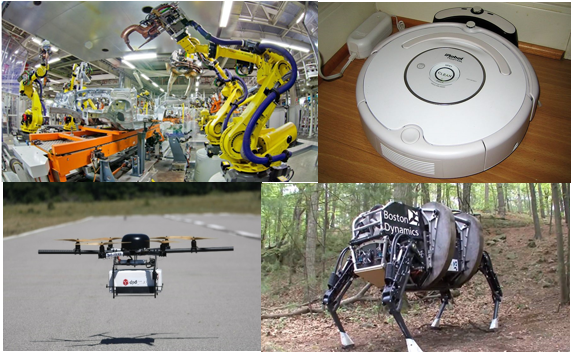
\includegraphics[width=0.7\textwidth]{figures/robots.png}
    \caption{Aplicaciones actuales de los robots.}
    \label{robots}
\end{figure}

Con el paso de los años se observa una clara tendencia hacia el diseño de sistemas robotizados para cubrir necesidades o desempeñar tareas que nunca se imaginaron automáticas. Surge, con ello, una necesidad social que requiere la instrucción de nuevos profesionales y expertos en esta potente rama de la ciencia y la tecnología que puedan lidiar con el diseño y desarrollo de estas entidades mecánicas cuyo comportamiento se espera que sea cada vez más complejo y completo, ayudando a los seres humanos no sólo a reducir costos, sino también a simplificar tareas, optimizar recursos y contribuir en labores de investigación. Es por eso que aumentan considerablemente aún hoy las ramas de estudio asociadas a la Ingeniería Automática, Mecánica, Electrónica y de Telecomunicaciones principalmente, que persiguen precisamente cubrir esa exigencia de formación para abordar un futuro lleno de robots, a la par que contribuyen a la generación de investigadores y proyectos que propulsarán el desarrollo de este sector en búsqueda del beneficio social. 

Las circunstancias idóneas para la instrucción e investigación necesario para el estudio de la Robótica no resultan sencillas de conseguir. Como ya se ha dicho, nuestro entorno actual engloba robots en grandes cantidades, pero también es cierto que el acceso a los mismos está muy restringido a cierto sector social. No se trata de un problema económico en cuanto a su adquisición, pues poco a poco el precio de producción de sistemas robóticos se reduce gracias al abaratamiento de componentes electrónicos y materiales con los que se elaboran, además de la optimización de los procesos de construcción y ensamblado de los mismos, que hacen que el precio final de los robots sea, en cierta medida, asequible para el consumidor medio dependiendo siempre de la aplicación. El problema reside más bien en que las circunstancias y los entornos de desarrollo, investigación, docencia e instrucción en la robótica son a la vez difícilmente accesibles, escasos, enormemente controlados y por último, pero quizá más importante, económicamente exigentes. Es por eso que resulta complicado el proceso de instrucción en robótica. Jamás pediríamos al escultor que aprendiera a esculpir sin cincel, o al biólogo que estudiase la naturaleza en su sótano. Sin embargo, debido al bajo grado de accesibilidad de los entornos docentes y de investigación en el campo de la robótica, en muchas ocasiones se priva de su principal herramienta de aprendizaje a los estudiantes e investigadores del campo, o se complica en gran medida su curva de entrada. En base a mi experiencia reciente puedo decir que el énfasis se pone, inevitablemente, ``sobre el papel'' en lugar de ``en la masa''.

Destaca también la carencia o escasez de entornos de aprendizaje graduales como los existentes en otros ámbitos, donde se comienza por un nivel básico que poco a poco se va incrementando. La robótica requiere, por definición, de entornos de aprendizaje e investigación altamente especializados, donde el usuario debe conocer de antemano no sólo los fundamentos básicos de los sistemas robotizados, sino también las nociones necesarias de matemáticas, física, mecánica y electrónica como mínimo, pudiendo extenderse el repertorio según el área de especialización dentro del campo.

Quedan de manifiesto las dificultades a las que se enfrenta todo aquel que quiere tener relación con la robótica.

\section{Tecnologías Web}

El crecimiento exponencial al que está sujeta la Web en los últimos tiempos hace que se vaya constituyendo un entorno ideal para el desarrollo de nuevas aplicaciones en lo relacionado con el ocio, los servicios y las necesidades de las personas. De entre los nuevos productos web más influyentes podemos encontrar ejemplos como Netflix, un servicio de video bajo demanda (VoD) que ofrece películas y series en \textit{streaming} a través de la web, o Spotify, de características similares en el caso del contenido musical, e incluso servicios de computación en la nube como Amazon Web Services sobre los que se puede construir cantidad de potentes plataformas que sirven a las personas a través de Internet como Dropbox, HootSuite o Foursqare.

Algunos años atrás resultaba impensable plantear un desarrollo robótico empleando este tipo de tecnología dado que los motores web apenas tenían potencia de cómputo suficiente para reproducir un vídeo, y mucho menos podían si quiera superar los límites del navegador para acceder a dispositivos externos. Las nuevas aplicaciones de las tecnologías web han demostrado que esta circunstancia ha cambiado hasta tal punto en que se pueden crear aplicaciones tan exigentes como juegos en realidad virtual, procesamiento de imágenes, la comúnmente llamada ``minería de datos'' o KDD e incluso tareas de aprendizaje automático gracias, entre otras cosas, a la posibilidad de acceder al \textit{hardware} de aceleración gráfica por parte del navegador y a la incorporación en el mismo de potentes núcleos o motores de ejecución, dando lugar a las aplicaciones dinámicas en la nube (Fig. \ref{web}).

\begin{figure}[!hbtp]  \centering\noindent
    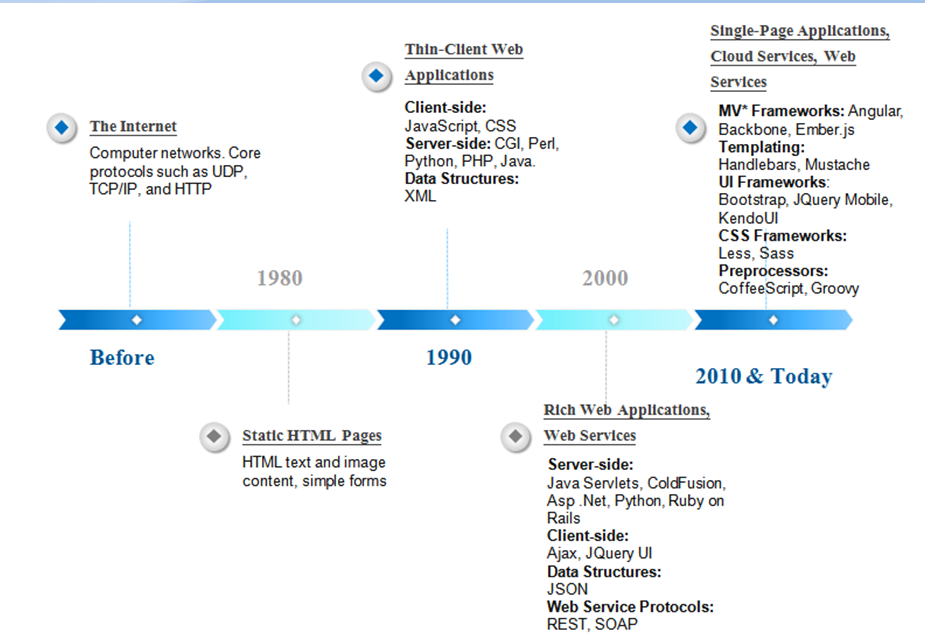
\includegraphics[width=0.99\textwidth]{figures/web-history.png}
    \caption{Evolución de las Tecnologías Web}
    \label{web}
\end{figure}

En la actualidad, se puede construir aplicaciones para casi cualquier caso de uso, incluido el de la robótica, completamente formados por herramientas web. Gran parte de sus ventajas residen en que el acceso a la web es totalmente público y sencillo, de tal manera que un servicio ofrecido a través de la web puede ser usado por cualquier persona del planeta, con independencia de su sistema operativo, dispositivo o entorno. 

Dado que Internet no es más que un conjunto debidamente interconectado de sistemas y redes de sistemas que se comunican a través de protocolos conocidos (mirándose con un gran nivel de abstracción), se puede conseguir de manera bastante eficaz conectar herramientas de distinta naturaleza para que funcionen como un conjunto homogéneo a través de Internet. Entre las funciones interconectables que nos ofrece la web, destacamos especialmente el acceso al \textit{hardware} del equipo cliente, el soporte de almacenamiento en la nube, los mecanismos de seguridad, las características de sus canales de comunicación (baja latencia punto a punto, retransmisiones, baja tasa de error y de paquetes perdidos,...) y la capacidad de ejecutar el código de la aplicación. 

Aún con todas las ventajas ya mencionadas, la característica responsable del éxito de las aplicaciones web es probablemente la facilidad de acceso que, como ya se ha dicho, se realiza a través de un navegador web. Este es el agente que tiene visibilidad tanto interna como externa, es decir, que puede comunicarse tanto con el PC o sistema en el que está instalado como con el resto del mundo, y funciona con independencia del sistema latente bajo él. Esto quiere decir que cualquier ente conectado a Internet puede acceder a las aplicaciones web, sin importar cuál sea su sistema. 

\section{Robótica a través de las Tecnologías Web}

La intersección entre el campo de la robótica y las herramientas web dispone un entorno con un gran potencial para el desarrollo de aplicaciones que permitan enfrentarse a tareas de investigación y aprendizaje con características muy atractivas.

\begin{figure}[!hbtp]  \centering\noindent
    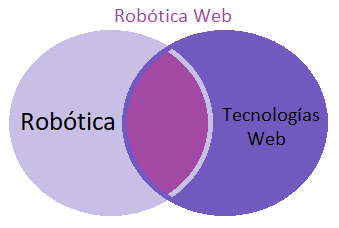
\includegraphics[width=0.55\textwidth]{figures/intersection.png}
    \caption{Entorno Robótico en la Web}
    \label{web}
\end{figure}

Investigando el panorama docente y de experimentación moderno en cuanto a robótica se refiere, encontramos numerosas librerías que ya facilitan en gran medida el trabajo con robots, como pueden ser OpenCV para tareas de Visión Artificial u OMPL para planificación de rutas, y también entornos de desarrollo y \textit{frameworks} que simplifican el proceso como ROS o YARP. 
Sin embargo, aún no se han desarrollado herramientas maduras que engloben estas nuevas tecnologías en una sola para que el trabajo con sistemas robóticos sea casi tan fácil como pulsar un botón y ver el código en acción. Hasta el momento, es necesario disponer de numerosos módulos inteligentes cuidadosamente interconectados que sincronicen y supervisen la ejecución de diferentes aspectos para lograr controlar cualquier aspecto de un robot, todos ellos necesariamente ideados y construidos por el sujeto que trata de desarrollar algo.

Aún no existen plataformas de uso extendido o estándar ``\textit{de facto}'' que permitan una buena instrucción en este joven campo de la ingeniería, siendo en muchos casos debido a que resulta muy difícil acceder a \textit{hardware} adecuado para el aprendizaje o investigación por temas económicos o restricciones externas, o llevar los conocimientos teóricos a un entorno práctico para asentar los conocimientos. Analizando el estado actual se ha encontrado algunas plataformas que ya buscan una primera aproximación hacia esa aplicación de propósito general en docencia e investigación, que tratan de disponer de todo lo necesario para que sentarse a programar un robot, o varios, resulte incluso sencillo, a la par que instructivo y alentador. Algunos ejemplos son:

\begin{itemize}

\item [$\rightarrow$] La herramienta \textit{Colaboratory}\footnote{\url{https://colab.research.google.com/notebooks/welcome.ipynb}} de Google es un entorno que permite escribir y ejecutar código, guardar el desarrollo y compartir su análisis por distintos medios, y que tiene funciones que permiten utilizar el \textit{hardware} de aceleración gráfica del equipo que accede a la aplicación para realizar tareas de gran consumo de cómputo haciendo uso de recursos informáticos muy potentes, todo desde el navegador. Está construida sobre el proyecto \textit{Jupyter}, que a su vez se ejecuta completamente en la nube, y se utiliza mayoritariamente para el desarrollo  de aplicaciones que tienen que ver con el \textit{Deep Learning}. Así, la gran ventaja que ofrece es que permite a los usuarios descargar su código sobre su propia tarjeta gráfica para acelerar los procesos (Fig. \ref{colab}).
\begin{figure}[!htbp]  \centering\noindent
    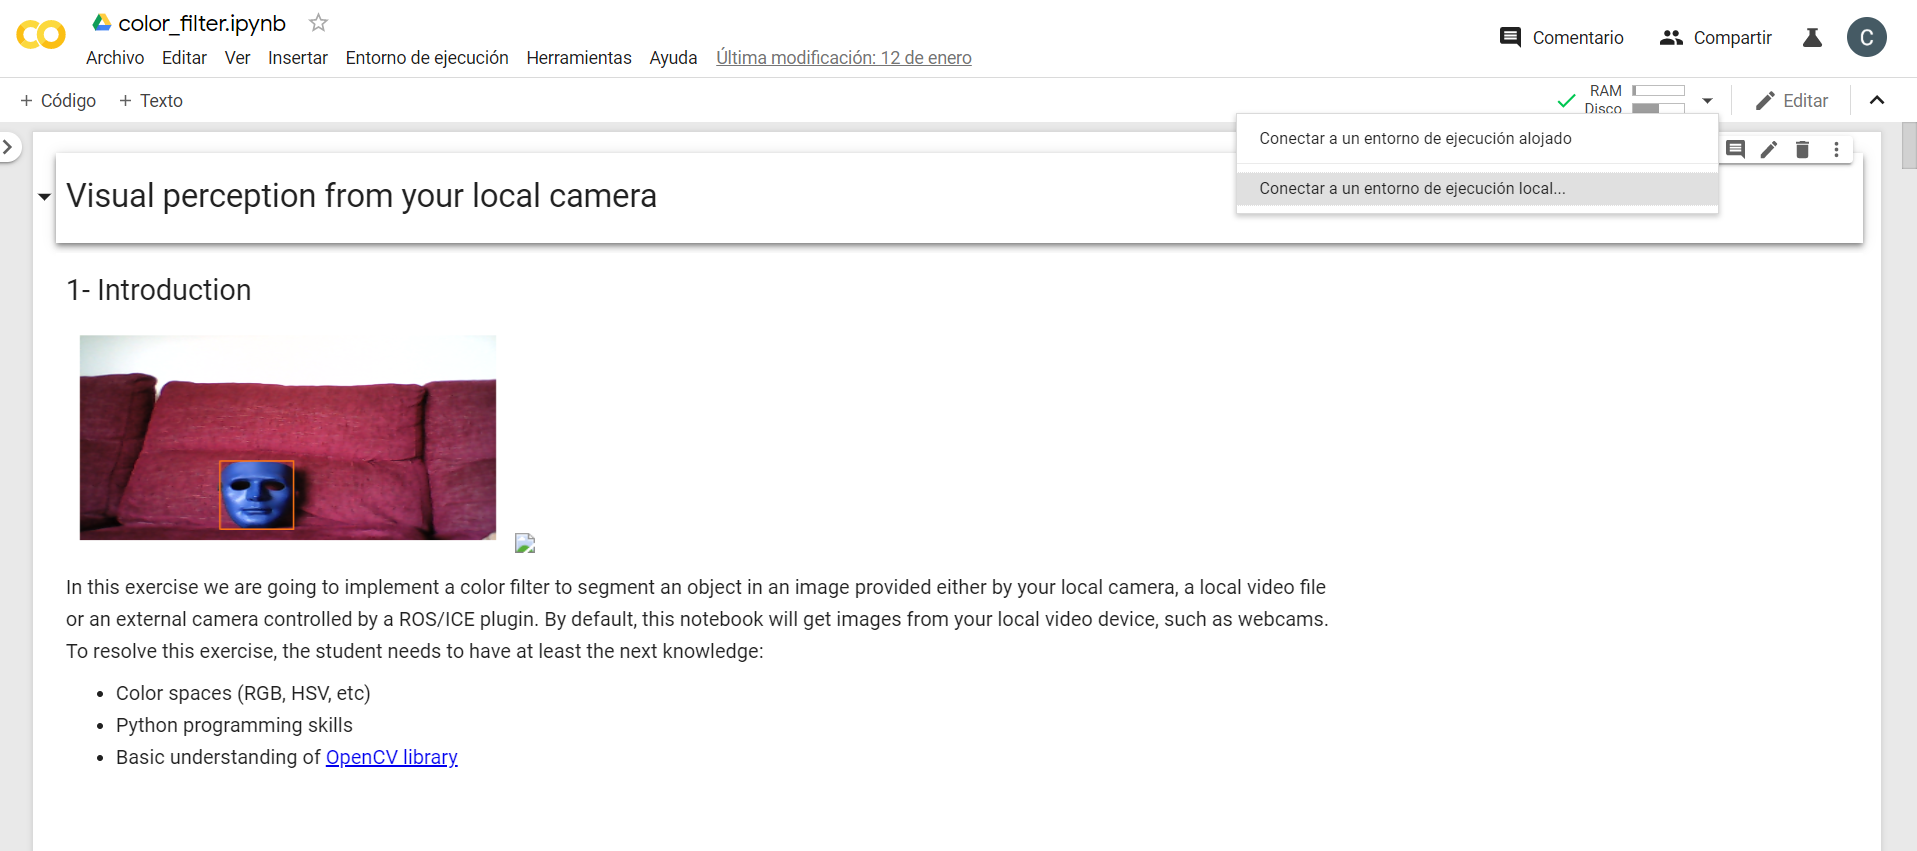
\includegraphics[width=0.99\textwidth,height=7cm]{figures/colab.png}
    \caption{Conexión Local de Colaboratory}
    \label{colab}
\end{figure}
\item [$\rightarrow$]Una plataforma con un gran potencial es la ``\textit{Robot Ignite Academy}\footnote{\url{https://www.robotigniteacademy.com/en/teachers/}} de la empresa The construct \footnote{\url{https://www.theconstructsim.com/}}. Esta plataforma, orientada sobre todo al aprendizaje relacionado con ROS y a las buenas prácticas de trabajo con robots, es una plataforma \textit{on-line} de pago cuyo uso objetivo es principalmente docente para equipos de trabajo o desarrollo en empresas, o para estudiantes de todo el mundo. Busca instruir a los usuarios en entornos prácticos simulados de aprendizaje en forma de cursos de distintos niveles, todos ellos con gran cantidad de detalle para una buena formación. Entre los servicios que oferta, se incluye la construcción desde el principio de un módulo robótico programable cuyo valor docente es importante. Entre sus características destaca que es completamente basado en tecnologías web, y por lo tanto accesible para cualquiera que disponga de un navegador. El rango de robots y escenarios que soporta es limitado (Fig. \ref{theconstruct}).
\begin{figure}[!hbtp]  \centering\noindent
    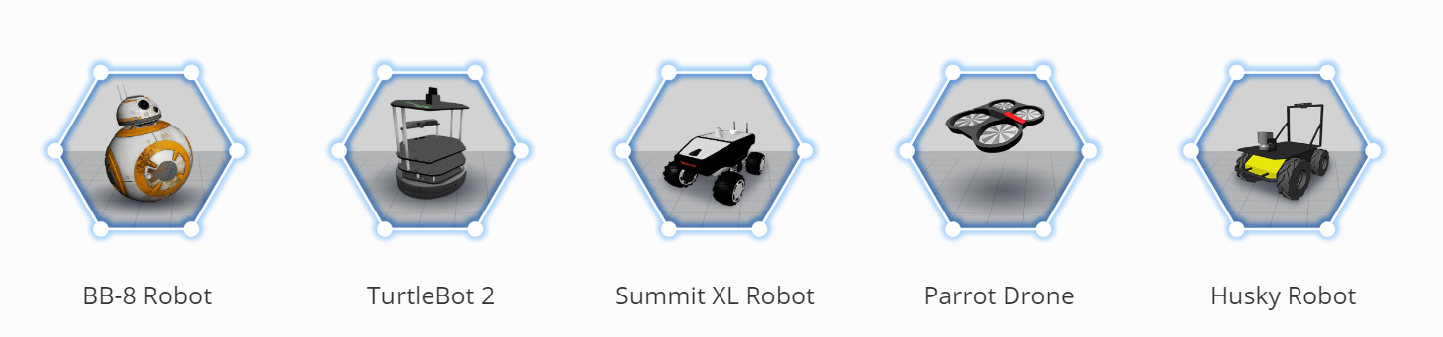
\includegraphics[width=0.95\textwidth]{figures/theconstruct.png}
    \caption{Robots Simulados soportados en Robot Ignite Academy.}
    \label{theconstruct}
\end{figure}
\item [$\rightarrow$] Otro gran ejemplo muy reciente es el entorno \textit{AWS RoboMaker}\footnote{\url{https://aws.amazon.com/es/robomaker/}} de Amazon. Se trata de un servicio que integra herramientas de trabajo con robots, como ROS y entornos de simulación robóticos, que además aprovecha la conectividad en la nube para ofrecer otros servicios, todos ellos propiedad de la empresa, que de nuevo cobra por el servicio que ofrece. Este entorno tiene muchas ventajas en cuanto al proceso de desarrollo e implementación de aplicaciones robóticas inteligentes a gran escala, además de facilitar el proceso de test para probar las aplicaciones que se construyen. Ofrece simulaciones muy realistas y entornos complejos para los robots, de tal manera que se pueden desarrollar comportamientos muy potentes, todo ello en simulación (Fig. \ref{awsrm}). No ofrece soporte para robots reales, aunque sí proporciona un servicio de administración de flotas que simplifica en gran medida el paso de la simulación al sistema físico. Se trata de un entorno web.

\begin{figure}[!hbtp]  \centering\noindent
    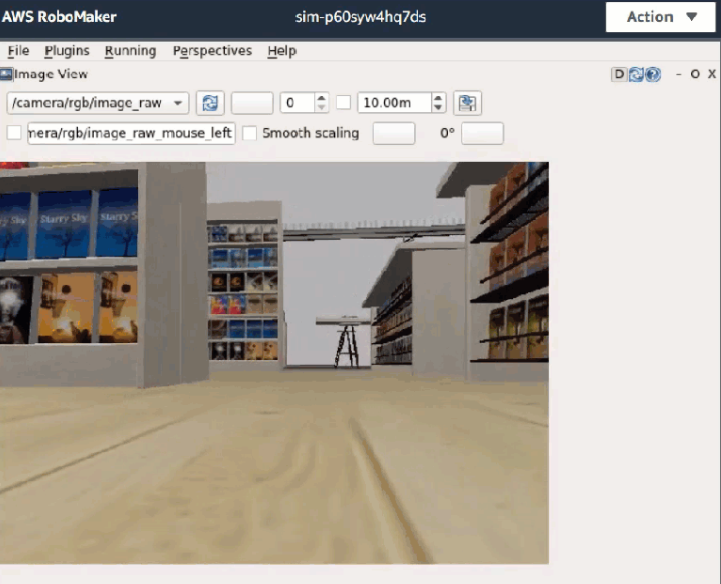
\includegraphics[width=0.8\textwidth]{figures/aws_robomaker.png}
    \caption{Simulación con AWS RoboMaker.}
    \label{awsrm}
\end{figure}

\item [$\rightarrow$] Existen otro tipo de plataformas menos extendidas, en el ámbito nacional e internacional, como JdeRobot\footnote{\url{http://jderobot.org}}, un entorno basado en componentes que se ejecutan como procesos que requiere instalación, y que se especializa en la disposición de todos los elementos necesarios para la fácil construcción de aplicaciones con robots y visión artificial. Si bien soporta tanto robots simulados como reales, este soporte es también limitado (repertorio concreto) y opera sobre las distintas distribuciones del sistema operativo Ubuntu, siendo que en el resto de casos es necesario recurrir a herramientas de virtualización para poder utilizarlo. Este entorno es muy completo y de código abierto, por lo que cualquier usuario puede acceder a él y utilizar toda su funcionalidad. A pesar de su filosofía de \textit{software libre} ofrece calidad profesional (Fig. \ref{jderobot}) a través de la integración de herramientas clásicas de desarrollo robótico como ROS, el simulador Gazebo, las librerías OpenCV y OMPL, etc. Aunque la aplicación es gratuita, requiere amplios conocimiento de programación de robots avanzada para trasladar el código de la simulación al sistema físico.

\begin{figure}[!hbtp]  \centering\noindent
    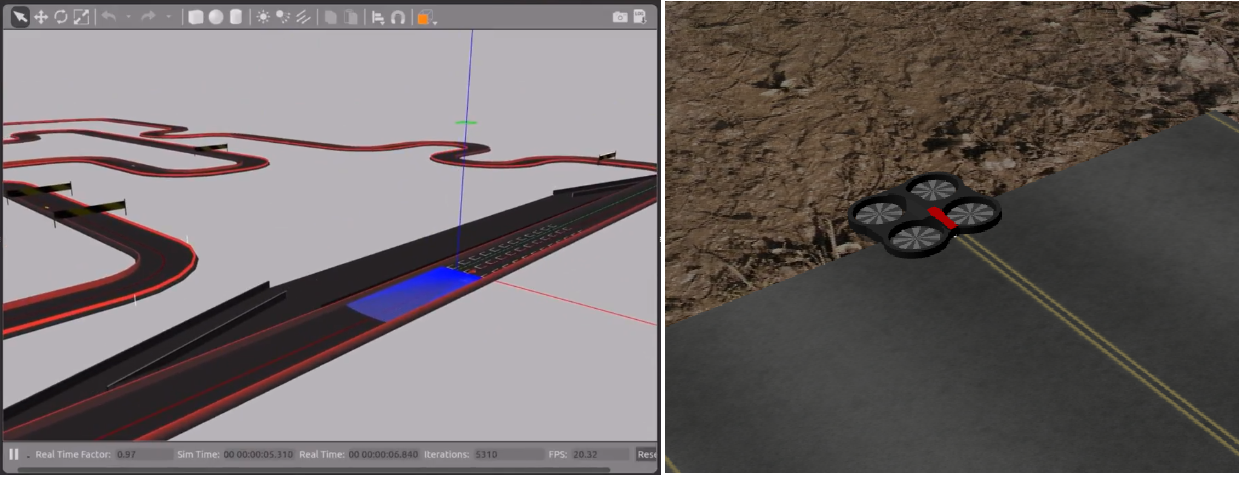
\includegraphics[width=0.8\textwidth]{figures/jderobot_simulation.png}
    \caption{Simulación de aplicación robótica con JdeRobot.}
    \label{jderobot}
\end{figure}

\end{itemize}

Inferimos que hay algo que todos ellos tienen en común: tanto su accesibilidad como su uso son limitados. Las carencias de los entornos actuales radican principalmente en que la mayoría son de pago, muchos de ellos sólo permiten el trabajo en simulación y la totalidad de ellos son incompletos, especialmente en el sentido de que sólo permiten trabajar en un área de la robótica, sólo con un tipo de robot (o una clase) o sólo permiten resolver ciertos problemas para los cuales se prepara un escenario muy controlado. Se observa, aún así, una clara tendencia a ofrecer este tipo de servicio de construcción de aplicaciones como \textit{middleware} a través de la nube para hacerlo más accesible, lo cual supone un punto a tener en cuenta a la hora de evaluar la situación actual y diseñar una nueva idea que colecte y compacte lo mejor de cada uno de los proyectos listados que existen a día de hoy. Es precisamente aquí donde se forma el lugar común entre robótica y tecnologías web, dando paso al entorno que alojará muchas de las aplicaciones robóticas del futuro próximo.

\section{Planteamiento del Problema}

El problema a tratar en esta tesis proviene del análisis de los factores que hacen distinto el desarrollo y el aprendizaje en este campo, y de cómo estos factores suponen un obstáculo, y en ocasiones incluso un impedimento, a la hora de realizar un proyecto específico. En este punto cabe preguntarse por qué no existen infinidad de plataformas y herramientas en la nube dotadas de aquellas características deseables para el aprendizaje y la investigación en el ámbito de los robots. 

Por un lado está el ya mencionado factor económico. Si nos paramos a pensar en el motivo por el cual las plataformas existentes se plantean como un servicio por el que hay que pagar caemos en la cuenta de que, aunque haya una parte debida al coste de desarrollo de dicha plataforma y al valor estratégico del producto que cubre una necesidad global en auge, principalmente se debe al consumo de recursos asociado a cualquier proyecto robótico en cualquier ámbito. Trabajar en robótica es sinónimo de disponer de recursos. Es bien sabido que el \textit{hardware} es caro y frágil, que la implementación tanto del sistema físico como de la lógica programada es temporalmente costosa y que incluso con la ausencia de sistemas reales, el coste computacional es enormemente elevado debido a que están involucrados programas exigentes como los simuladores robóticos y también dada la necesidad de un control estricto y veloz de todos los submódulos que componen un proyecto robótico, cada uno de ellos encargado de una tarea que requiere de más y más capacidad para realizar operaciones por unidad temporal. El primer obstáculo encontrado durante el análisis fue precisamente que \textbf{el consumo de recursos genera costes}, y que estos costes son elevados.

Por otro lado, en mi opinión, aprender robótica exige robots. Ya no sólo desde el punto de vista económico sino también desde el logístico, es complicado crear un servicio que disponga de tantos robots como usuarios y que pueda acarrear con los costes derivados de su uso por todo el que lo requiera. Aún pudiendo afrontarlos, construir un sistema que permitiese al usuario, sea estudiante, investigador o simple curioso, evaluar el código de su aplicación sobre un elemento \textit{hardware} remoto y acceder a los resultados en tiempo de ejecución sería una ardua tarea. Por tanto, el análisis realizado destacó que \textbf{desarrollar aplicaciones robóticas requiere disponer de realimentación, visual y paramétrica, en tiempo real}, sólo alcanzable a través de la observación de sistemas electro-mecánicos reales.

Por último, generalmente se desarrolla una gran cantidad de herramientas y plataformas que soportan sistemas específicos, es decir, de funcionalidad acotada. Esto supone un problema para el usuario medio ya que, normalmente, \textbf{carece de \textit{hardware} específico. Sin embargo, sí que tiene acceso a sistemas más básicos}. Esta circunstancia resultó ser la tercera clave extraída del estudio previo.

Así las cosas, la conclusión a la que se llegó es que no existen actualmente herramientas que simplifiquen el uso docente y de investigación de la robótica. Con todo lo anterior y sin perder de vista la idea de ``Acercar la robótica a la gente'', el problema radica precisamente en sortear esos obstáculos.

	\chapter{Objetivos y Metodología de Trabajo}

Este capítulo detallará los objetivos impuestos tras el trabajo de análisis inicial que se pretende alcanzar mediante los periodos de investigación e implementación de esta tesis de fin de Máster. Se describirá brevemente lo que se quiere abordar y cómo se pretende hacer, además de incluir otros sub-objetivos que surgieron durante el desarrollo reservando los detalles de los mismos para el punto en el que sea relevante. Así mismo, se expondrá la metodología bajo la que se organizó el proyecto.

\section{Proyecto Planteado}

Esta sección se reserva para exponer la idea objeto de esta tesis y la motivación o motivaciones principales que han llevado a su desarrollo, de vital importancia para comprender qué se pretende conseguir con ella y por qué se escogió esta idea y no otra.

La \textbf{``Ejecución Mixta''} para proyectos de robótica y visión artificial surge de la conjunción de las ideas planteadas en el capítulo anterior, persiguiendo incrementar la accesibilidad de la robótica y su aprendizaje. Se busca elaborar una herramienta que pueda ser conectada de manera modular con cualquier aplicación de carácter robótico y con soporte para cualquier usuario, sean cuales sean sus circunstancias.

Esta idea se planteó como una serie de características intrínsecas que dan forma a los objetivos que se quiere lograr. En tanto que se quiere facilitar el uso de la robótica, deberá existir un Interfaz de Programación o API que abstraiga a los usuarios de todo lo relacionado con la infraestructura de la herramienta y la aplicación, de los mecanismos de comunicación con los sistemas involucrados (tanto robots como sensores y PCs, servidores, \textit{proxys}, etc.) y del control de flujo propio de un sistema complejo, permitiéndole centrarse en su tarea específica de desarrollar con robots. Además, dado que los usuarios potenciales no desean suponer costes sobre los constructores de las aplicaciones que necesitan usar para su trabajo o estudio y que tampoco quieren que se les cobre su utilización (debido en muchos casos a que no se pueden afrontar tasas a largo plazo sin resultados prometedores en plazo corto), la idea que se expone debe estar orientada al cliente, siendo este el que acarree con toda la carga de cómputo posible y asuma el consumo de recursos, que utilizará a su conveniencia según la disponibilidad de la que goce.

La herramienta final objetivo constituirá una forma de lograr no sólo la ejecución de código específico accediendo a un único elemento \textit{hardware} concreto de la máquina cliente, sino la ejecución de aplicaciones robóticas completas de cualquier ámbito en cualquier dispositivo \textit{hardware} del que el cliente disponga, incluso si éste está conectado a través de un puerto USB o una red WiFi (ya sea un ordenador, sensores, un robot, etc.) mientras el código se almacena remotamente y se ofrece al usuario a través de la nube, por medio de las tecnologías web. Bajo esta filosofía el código o la aplicación desarrollada por el cliente a través de la web se almacena en un servidor remoto, pero éste sigue teniendo acceso a su análisis y resultados al ejecutarse en sus propios equipos y sistemas robóticos locales, quedando todas las tareas de bajo nivel involucradas en la aplicación robótica ``escondidas'' a nivel de usuario y solventadas por la aplicación que se sirve, como puede ser la comunicación entre servidor y cliente y el acceso a su \textit{hardware}, el diálogo entre el código implementado y robot (simulado o real) y con lo relacionado con el soporte gráfico (UI) y el entorno de trabajo, de modo que se dota al usuario de cierta abstracción de los temas que para él o ella son irrelevantes, permitiéndole centrar sus esfuerzos en idear y desarrollar la lógica que controle al robot y le permita abordar el problema que se propone.

La herramienta deberá encajar con aplicaciones docentes y de investigación, actuando más bien como una capa intermedia que hace las funciones de \textit{middleware} entre el robot del usuario y un sistema remoto.

\section{Objetivos del Proyecto}

Este trabajo esta compuesto por cuatro grandes objetivos impuestos en primera instancia, pudiendo todos ellos descomponerse a su vez en sub-objetivos de menor complejidad que sirven para disponer un escenario de trabajo inicial:

\begin{enumerate}
\item Realizar un profundo trabajo de investigación acerca de las herramientas, componentes y entornos más utilizados en los proyectos robóticos.
    \begin{itemize}
        \item Se trata de analizar las características de cada agente de estudio para poder elegir o descartar con criterio su incorporación al proyecto.
    \end{itemize}
\item Probar y seleccionar aquellas herramientas que puedan adaptarse al problema que se pretende resolver.
    \begin{itemize}
        \item Este hito pasa por construir diseños preliminares del entorno que engloba un cliente y un sistema remoto que se quieren interconectar.
    \end{itemize}
\item Construir una nueva solución de servicio web que cumpla la ``Ejecución Mixta'' en forma de módulo que resuelva un problema para el que aún no existe una solución clara.
    \begin{itemize}
        \item Este proceso supone a su vez la implementación de prototipos,
        \item nuevas etapas de investigación para el enriquecimiento del sistema y
        \item continuos procesos de supervisión para asegurar que el resultado contiene las características objetivo, que son:
            \begin{itemize}
                \item Accesible (Multiplataforma, Multilenguaje).
                \item Soporte para simulación y sistemas reales.
                \item Ejecución en el cliente.
                \item Fácil de usar.
                \item Versátil (Visión Artificial, Robots de cualquier clase).
            \end{itemize}
    \end{itemize}
\item  Llevar a cabo un exhaustivo programa de pruebas para evaluar la validez y la viabilidad de la idea planteada y su implementación.
\end{enumerate}

Estos objetivos establecen a su vez un esquema de trabajo que dictará la manera en que se desarrolla, realizando siempre una supervisión para garantizar que se cumple cada meta propuesta antes de pasar a la siguiente.

\section{Metodología Empleada}

Este proyecto se dividirá, principalmente, en dos partes bien diferenciadas: \textbf{etapa de investigación} y \textbf{etapa de implementación}. Estableceremos de antemano una serie de reglas que organizarán la manera en que se trabaja en ambas partes en busca de la mayor eficiencia y efectividad posible.

En cuanto al método de sincronización del trabajo se puede decir que se descompuso su elaboración en una serie de iteraciones fromadas por varias fases en las que, por medio de una reunión, se pusieron en común los avances obtenidos en cada período para evaluar el estado del proyecto y corregir posibles fallos, además de establecer los sub-objetivos siguientes, discutir la mejor manera de abordarlos y determinar los obstáculos que podían surgir de cara a la siguiente iteración. Esto no sólo constituye un método de trabajo fluido y completo, sino que además permite asentar bien los conocimientos adquiridos y puestos en práctica para resolver cada problema. Gracias a esta rápida realimentación, los errores no se propagan y las dudas se despejan con gran eficacia. Durante los intervalos de trabajo entre cada reunión, el seguimiento se hizo a través de una bitácora semanal \footnote{\url{https://github.com/cawadall/TFM-Carlos-Awadallah/blob/master/README.md}} donde se iba actualizando asiduamente el estado del proyecto a través de material audiovisual, \textit{snippets} de código y detalladas descripciones de lo hecho. Tanto esta bitácora como el código del proyecto, de carácter abierto, estuvo en todo momento accesible para los tutores, con lo cual se podían preparar las reuniones de antemano e incluso intercambiar ideas y sugerencias de manera anticipada \footnote{\url{https://github.com/cawadall/TFM-Carlos-Awadallah}}.

\subsection{Metodología de Investigación}

Dado que estamos tratando de abordar un problema para el que aún no existe una solución, gran parte del proyecto se dedicó a la investigación. Se hizo necesario reunir la documentación asociada a una gran cantidad de herramientas y proyectos en auge que reunían algunas de las características que buscábamos. Para abordar esta parte del trabajo, tratamos de realizar una primera pasada escogiendo todas aquellas opciones que contaran con al menos una de las características que habíamos establecido como objetivo. A partir de este punto, realizamos numerosos ciclos, cada uno de ellos con su respectivo proceso de testeo, para filtrar en primera instancia todas aquellas que fueran poco maduras, incompletas o que no encajasen con los requisitos de nuestro proyecto, y luego se trató de descartar, en un último ciclo, los peores candidatos entre las herramientas finalistas en base a una evaluación del porcentaje de superposición entre el conjunto de prestaciones de la herramienta y el set de características que habíamos establecido.

Esta filosofía se respetó hasta el comienzo de la implementación punto a partir del cual cualquier tarea que requiriese volver a investigar se produjo simplemente con la idea de resolver un problema muy concreto o mejorar algún punto del trabajo.

\subsection{Metodología de Implementación}

Para la consecución del resto de objetivos se optó por la filosofía de Barry Boehm del modelo de desarrollo en espiral \cite{BB1986}. Este método busca separar el comportamiento objetivo en diferentes sub-tareas de menor complejidad conservando la flexibilidad ante nuevos objetivos que surjan durante el desarrollo o sucesos no previstos y requisitos variantes, circunstancias que suelen estar presentes en la mayoría de proyectos de este calibre. Así, se consigue fijar la arquitectura y el flujo de trabajo en la fase inicial e ir construyendo la aplicación gradualmente mientras se verifica simultáneamente la calidad en cada paso (Fig. \ref{espiral_bb}).

\begin{figure}[!htbp]  \centering\noindent
    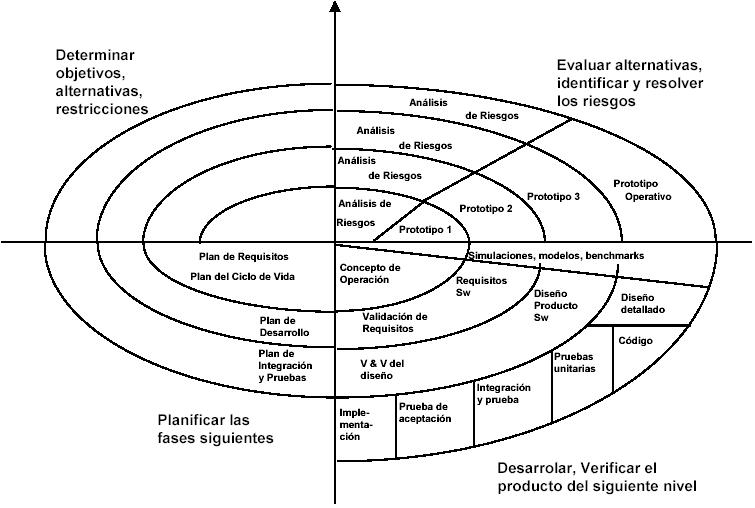
\includegraphics[width=0.95\textwidth]{figures/espiral_boehm.jpg}
    \caption{Modelo en Espiral del Proceso de Desarrollo Software.}
    \label{espiral_bb}
\end{figure}

Gracias a la estructura cíclica se consigue tener un prototipo funcional que va creciendo en riqueza y complejidad en cada pasada, construyéndose cada vez sobre el prototipo de la iteración anterior para abordar los objetivos de ciclo, a través de los cuales se consigue mejorar el desarrollo y, en última instancia, pulirlo para cubrir todos los requisitos planteados y obtener la versión final. Cada fase del desarrollo incremental se divide en 4 fases bien definidas por las que el proyecto debe pasar:
\begin{enumerate}
    \item \textbf{Determinar los objetivos del ciclo}. Esta primera fase consiste en definir las metas que se pretende alcanzar en el ciclo. Estas metas son a su vez las que determinan cuándo se da por finalizada la iteración.
    \item \textbf{Análisis del riesgo}. En segundo lugar se trata de analizar los objetivos propuestos en búsqueda de las partes más delicadas para determinar qué problemas u obstáculos pueden surgir durante el desarrollo y planificar cómo abordarlos.
    \item \textbf{Desarrollar y probar}. Con un plan de desarrollo definido en base a los riesgos potenciales, y con los objetivos de ciclo presentes, se comienza con la implementación. También ha de pasarse el correspondiente \textit{set} de pruebas para garantizar un desarrollo funcional y completamente operativo.
    \item \textbf{Planificación de la siguiente fase}. Para acabar, se evalúan los resultados obtenidos en la etapa actual del proyecto y se comienza con la planificación de las próximas fases del proyecto.
\end{enumerate}

	\chapter{Infraestructura Utilizada}

Este capítulo recoge el conjunto de herramientas seleccionadas para este proyecto, así como una detallada descripción de la relación entre unas y otras. Se introducirá cada una de las herramientas y se especificará tanto las razones de su elección para el proyecto como la función que cumplirá en él.

Lo que se recoge a continuación es el resultado de los meses de investigación, en los cuales estudiamos numerosas herramientas, entornos y plataformas aplicables a la robótica web que podían aportar algo a nuestros intereses. Finalmente se escogieron los que se listan en este tercer capítulo para formar parte de la solución de ``Ejecución mixta'' para aplicaciones robóticas que proponemos en este Trabajo Fin de Máster.

\section{Proyecto Jupyter}

La herramienta fundamental en la que se basa este desarrollo es el proyecto Jupyter\footnote{\url{https://jupyter.org/}}, la evolución de \textit{IPython 3.0}. Se trata de una aplicación web de código abierto que ofrece la capacidad de crear y compartir documentos, llamados cuadernillos o \textit{Notebooks}, los cuales puede contener textos narrativos y elementos de texto enriquecido (párrafos, ecuaciones, figuras, enlaces, etc.), imágenes ilustrativas, códigos empotrados, ecuaciones, visualizaciones (figuras, gráficos, tablas, etc.) y gran cantidad de elementos gráficos inteligentes. La razón principal de su elección, además de por pertenecer al ámbito de las tecnologías web, es que además de empotrar y editar código el usuario puede ejecutarlo desde su navegador, gracias a la comunicación implícita de la aplicación con los núcleos o \textit{kernels} de computación que incluye el sistema, incluyendo intérpretes para distintos lenguajes. Con ello se dispone de una herramienta a través de la cual se pueden llevar a cabo potentes tareas como la transformación de datos, el modelados estadístico de los mismos, simulaciones numéricas, visualización y análisis de los datos y aprendizaje automático, siendo todos ellos sus principales usos, aunque su funcionalidad es mucho más amplia.

La característica principal del entorno son sus \textit{Notebooks}, documentos generados a través del interfaz de usuario que pueden contener todo lo anteriormente mencionado, completamente legibles por usuarios humanos pero con capacidad para ejecutar código de computadora en hasta 100 lenguajes diferentes para los que da soporte en la actualidad. Básicamente consisten en una
secuencia lineal de celdas que pueden ser de diferentes tipos, dependiendo de su contenido:
\begin{itemize}
\item Celdillas de código: entrada y salida del código en el lenguaje seleccionado para el \textit{Notebook} que se ejecuta en el \textit{kernel}. Estas celdas son extensibles para poder visualizar el resultado de la ejecución del código especificado.
\item Casillas de reducción: contienen texto narrativo con ecuaciones en formato LaTeX embebidas.
\item Encabezado de celdas: texto de 6 niveles de organización jerárquica y formato. Útiles para establecer títulos y subtítulos y obtener un documento mucho más claro y ordenado.
\item Celdas sin formato: texto sin formato específico para ser exportado a diferentes formatos mediante \textit{nbconvert} sin sufrir cambios.
\end{itemize}

\begin{figure}[!hbtp]  \centering\noindent
    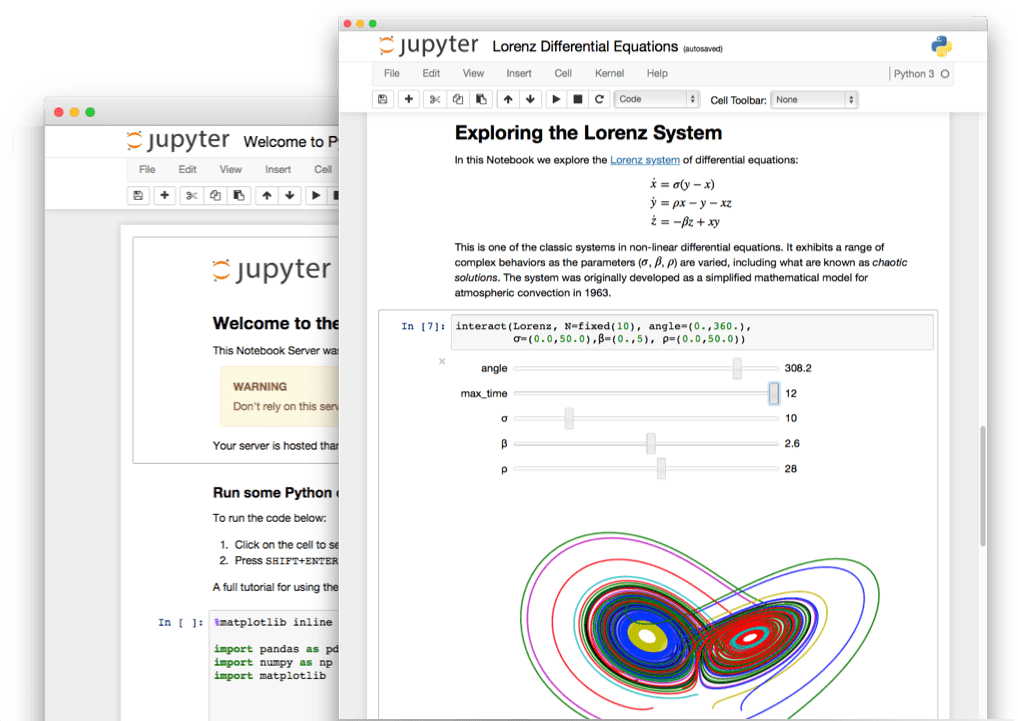
\includegraphics[width=0.8\textwidth]{figures/jupyterpreview.png}
    \caption{Cuadernillos de Jupyter}
    \label{jppreview}
\end{figure}

Se crean cuadernillos mediante la combinación de los elementos anteriores a través del navegador web, y la aplicación servidor-cliente permite editarlos y ejecutarlos dinámicamente. Para utilizar el servicio, se debe instalar su \textit{software} en un escritorio local y lanzar la aplicación, supuesto en el que no se requiere conectividad de red, o bien puede instalarse en un servidor remoto y utilizar Internet para el acceso. Además de mostrar, editar y ejecutar \textit{Notebooks}, el entorno dispone de un panel de control compuesto de una serie de instrumentos que ejercen alguna clase de acción sobre el cuadernillo, entre los que se encuentran las funciones de abrir y cerrar documentos, levantar, borrar o reiniciar un núcleo, cambiar el formato de una celda concreta o sus meta-datos, etc.

Quizá la parte más importante de esta aplicación son los \textit{kernels} que se han mencionado. Se trata de ``motores computacionales'' que ejecutan el código que el usuario escribe en el cuadernillo. Corrigen la sintaxis del lenguaje y devuelven una serie de instrucciones en código máquina que pueden ser ejecutadas, evalúan su resultado y lo disponen para que el usuario tenga acceso a él a través del interfaz, tal y como haría un intérprete en el caso de los lenguajes interpretados y la secuencia de un compilador y un ejecutor en el resto de casos. Cuando se inicia un \textit{Notebook}, el \textit{kernel} asociado (especificado automáticamente en los meta-datos del documento) se levanta automáticamente, de manera que al ejecutar cada celdilla con código éste realiza el cálculo y produce los resultados. Dependiendo del tipo de cálculos, el \textit{kernel}
puede consumir CPU y RAM significativas (siempre de la máquina en la que se está ejecutando la aplicación), pudiendo ejecutar procesos más exigentes y desarrollar aplicaciones de mayor complejidad. Finalmente, los cuadernillos pueden ser guardados por el usuario en su sistema de ficheros local, como un documento con extensión \textit{.ipynb}.

Se han mencionado varias características muy interesantes de esta herramienta que encajan a la perfección con nuestros propósitos. En primer lugar, el \textit{kernel} aprovecha toda la capacidad de cómputo del sistema del cliente en que se levanta la aplicación, es decir, puede utilizar su sistema a su conveniencia en función del código que ejecuta. Esto significa que tiene la capacidad de acceder al \textit{hardware} del usuario y de actuar sobre él, justo lo que necesitamos para el proyecto que se presenta. Además, tal y como se especifica en la documentación, el interfaz de Jupyter puede ser accedido remotamente a través de un navegador si se conoce su origen. Eso supone que, aunque el código se está ejecutando en cliente, un agente remoto puede actuar sobre el documento y enviar la orden para que se ejecute de algún modo. Mediante la combinación de estas dos características obtenemos una herramienta que puede actuar de editor de texto para el código del usuario, y que proporciona herramientas para el acceso a su \textit{hardware} de modo remoto, siempre y cuando sea el usuario quien escribe el código. 

Los \textit{Notebooks} que ofreceremos en este TFM se basarán en código Python, versiones 2.7 o 3.5 según las necesidades. Hemos escogido este lenguaje dadas sus amplias ventajas en accesibilidad (mismo intérprete en distintos SO), su versatilidad, su potencia y su fácil adaptación con los mecanismos robóticos, siendo que existen numerosas librerías estándar en robótica con soporte para Python.

\section{Plataforma Docker}

Docker\footnote{\url{https://www.docker.com/}} es una plataforma integral de código abierto para desarrollar, enviar y ejecutar aplicaciones en un entorno virtualizado ligeramente aislado, de manera que aprovecha todas las ventajas y funciones que pone a su disposición un sistema operativo sin requerir todas las dependencias que en primera instancia hacen falta para una virtualización completa como la que se puede encontrar en la tecnología de máquinas virtuales. Docker permite separar la aplicación final de la infraestructura de desarrollo, de tal manera que el \textit{software} se puede compartir rápidamente. Incluso ofrece la capacidad de gestión de una infraestructura completa reduciendo significativamente el tiempo que transcurre entre la desarrollo de la aplicación y su puesta en marcha en un entorno de producción, eliminado los obstáculos que pueden surgir al llevar el código de una máquina a otra. Esto se consigue a través de unidades estándar de software capaces de empaquetar el código de una aplicación y todas sus dependencias para que se ejecute de forma rápida y fiable de un entorno informático a otro. Estas unidades reciben el nombre de contenedores Docker.

Los contenedores garantizan aislamiento y seguridad, lo que permite ejecutar varios contenedores simultáneamente en un \textit{host} determinado sin que se produzcan colisiones y protege el sistema anfitrión sobre el que se monta el contenedor. Además, como ya se ha dicho, son ligeros porque no necesitan la carga extra de un hipervisor, sino que se ejecutan directamente en el \textit{kernel} de la máquina anfitriona, lo que también supone que se superan los largos y tediosos procesos de instalación de la aplicación, sustituyéndose por una ligera descarga. La versatilidad de estas unidades de computación es muy elevada, permitiendo combinaciones complejas como construir una unidad de contenedor sobre un anfitrión que es una máquina virtual, sobre un centro de datos local, un proveedor de \textit{cloud computing} o incluso un híbrido entre ambos (Fig. \ref{docker}).

\begin{figure}[!hbtp]  \centering\noindent
    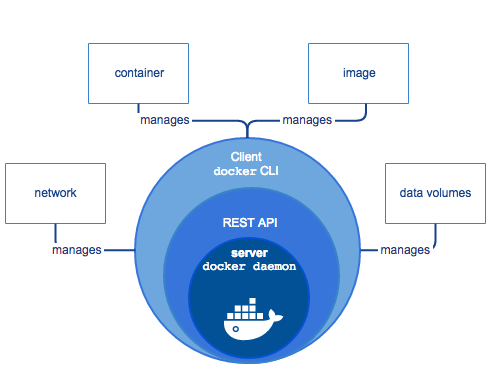
\includegraphics[width=0.8\textwidth]{figures/docker-engine.png}
    \caption{Estructura de Docker}
    \label{docker}
\end{figure}

Así, se puede decir que utilizar Docker multiplica exponencialmente la escalabilidad y portabilidad de una aplicación, ya que no hay que prestar atención el sistema operativo latente en el anfitrión, pues la infraestructura del contenedor configura el entorno que la aplicación necesita. Consideramos que esta característica puede resolver toda la parte de accesibilidad a la herramienta que queremos construir, en tanto que se pretende que ésta sea un cliente que se comunica con una aplicación robótica remota y que necesita disponer de ciertos recursos y ejecutar ciertas tareas en el sistema del usuario.

La necesidad de usar esta plataforma surgió a medida que avanzó el proyecto. Se usará en sustitución de la instalación en el ordenador del cliente de la parte de la plataforma web propuesta que es necesaria para que se ejecute en el ordenador del usuario el cómputo de las aplicaciones robóticas. Persiguiendo las ventajas de un proyecto multiplataforma e independiente del sistema del cliente, investigamos Docker para mejorar la experiencia de usuario al evitar que éste tenga que llevar a cabo procesos de instalación, en tanto que podríamos disponer uno con todo lo necesario para que el cliente disfrute de las funciones para aplicaciones robóticas que pueda necesitar desde un entorno predispuesto y debidamente configurado a través de un contenedor.

\section{Entorno Django}

Django\footnote{\url{https://www.djangoproject.com/}} es un marco de trabajo clasificado como tecnología de servidor de alto nivel en Python que garantiza el desarrollo rápido del lado servidor de una aplicación y su diseño. Ofrece gran cantidad de funcionalidad resuelta que se encarga de los detalles del desarrollo Web. Con Django se puede construir una aplicación reutilizando módulos de código con la funcionalidad típica de una aplicación, de tal manera que el desarrollo puede centrarse en escribir la lógica específica del servicio que quiere ofrecer sin necesidad de empezar desde el principio programando cada módulo. Es gratuito y de filosofía abierta.

La arquitectura de Django resulta bastante simple. Como se puede ver en la Figura \ref{django}, organiza la aplicación de tal manera que resulta muy sencillo conocer en todo momento el estado del proceso de servicio.

\begin{figure}[!hbtp]  \centering\noindent
    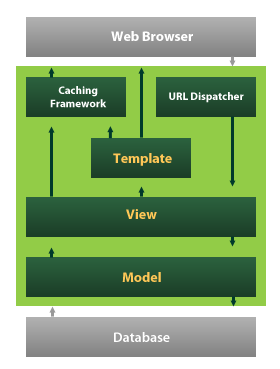
\includegraphics[width=0.65\textwidth]{figures/django-arch.png}
    \caption{Arquitectura de Django}
    \label{django}
\end{figure}

Se controla muy fácilmente lo que el usuario ve a través de las vistas de Django, con las que además se dota a la aplicación web de dinamismo e inteligencia. También se controla cómo ve el usuario el contenido de la aplicación a través de las plantillas, que proporcionan herramientas de interacción entre el usuario y el servidor y le permiten realizar peticiones simples para potenciar la funcionalidad que se puede ofrecer. Por último facilita mecanismos muy simples de gestión y acceso a bases de datos a través de distintas tecnologías como MySQL o MongoDB, necesarias para las aplicaciones y que evita la especialización en lenguajes utilizados para peticiones a bases de datos por parte del desarrollador web. En resumen, facilita el proceso de construcción y diseño de aplicaciones web para que el desarrollador no tenga que preocuparse por el bajo y medio nivel.

Esta característica, junto con la escalabilidad del lado servidor construido con tecnologías web de servidor, es precisamente la que decantó la balanza hacia el uso de Django en nuestra plataforma. La aplicación web resultante será enriquecida con la herramienta de ``Ejecución Mixta'' para ofrecer cierto servicio robótica docente. La aplicación remota basada en Django ofrecerá la funcionalidad para la que ha sido diseñada sin consumir recursos en el sistema anfitrión, y llevará a cabo el proceso de ``Ejecución mixta'' que queremos conseguir para garantizar el acceso a cualquier cliente.

\section{ROS (Robot Operating System)}

ROS (Robot Operating System)\footnote{\url{https://www.ros.org/}} es un \textit{middleware} flexible ideado para desarrollar \textit{software} robótico. Proporciona multitud de bibliotecas, paquetes de código y herramientas para ayudar a los desarrolladores de aplicaciones relacionadas con la robótica en todos sus ámbitos a crear aplicaciones de robots. Su uso está muy extendido por todo el mundo, desde caseros a profesionales, dadas sus ventajas frente a otros soportes similares. Su extensión se debe en parte a que surgió en una etapa en la que no existía un entorno abierto que unificara todos los módulos necesarios para construir una aplicación robótica completa, y en la que tampoco existía \textit{software} estándar para la programación de robots. En esos años el desarrollo de un proyecto en muchos casos se tornaba arduo, además de la complejidad presente a la hora de extenderlo, incluir herramientas o funcionalidad externa o incluso al agrandar el grupo de desarrollo, en el que cada uno podía tener su método de trabajo. ROS alivia todos estos problemas al ofrecer los módulos necesarios para implementar el código y llevarlo al robot, de principio a fin, todo en un mismo sitio distribuido bajo una licencia BSD de código abierto. Permite la abstracción de la capa \textit{hardware}, proporciona controladores de dispositivo (\textit{drivers} o \textit{plugins}), bibliotecas, visualizadores, resuelve el intercambio de mensajes y facilita la administración de paquetes entre muchas otras cosas.

Resulta bastante lógica su elección para este TFM, en el que precisamente queremos lograr esa abstracción del bajo nivel para ofrecer una plataforma de desarrollo de aplicaciones de alto nivel para que el usuario se sienta cerca de la robótica. Cabe destacar también que ROS ofrece soporte para distintos lenguajes, entre ellos Python, y que dispone de canales de comunicación automáticos configurables y parametrizables que simplifican en gran medida la comunicación con el \textit{hardware} y con aplicaciones externas.

En esta línea destaca otra de las fortalezas de ROS, que es su integración con el simulador Gazebo mediante la serie de paquetes \textit{gazebo\_ros\_pkgs}\footnote{\url{https://wiki.ros.org/gazebo\_ros\_pkgs}} que utilizan estructuras de tipo \textit{ROS Messages} para permitir la simulación de robots y  ofrecer servicios sobre la simulación como la reconfiguración dinámica. Esta ventaja puede ser muy útil para el soporte de simulación que queremos incluir en la solución de ``Ejecución Mixta'', para aquellos usuarios que no disponen de sistemas electro-mecánicos reales. ROS provee de los módulos \textit{software} que permiten controlar las interfaces de los robots simulados pero también reales, proporcionándonos acceso a sus sensores y control sobre sus actuadores.

ROS propone un desarrollo basado en la estructura de la aplicación organizada como una colección de nodos (procesos que conllevan computación) que se jerarquizan y se combinan en un grafo comunicándose entre ellos mediante \textit{topics} o canales de transmisión, servicios RPC y el Servidor de
Parámetros. Con esto, podemos ejercer un control específico y restrictivo sobre cada módulo implicado en el sistema de control de un robot, que generalmente comprenderá muchos, y ofrecer al usuario sólo aquellos que necesita en cada ocasión para facilitarle el desarrollo. El empleo de nodos en ROS proporciona  beneficios como la tolerancia adicional a errores (quedan contenidos en nodos individuales) y la disminución de la complejidad del código.

En cuanto a los \textit{topics} como medio de comunicación, se definen como buses que los nodos utilizan para intercambiar mensajes con formatos específicos. Tienen una semántica  basada en la publicación de mensajes y/o suscripción anónima a un canal concreto o varios, que desacopla el cómo o quién genera cierta información del quién o qué la consume. Con ello, los nodos no tienen por qué saber la fuente o el receptor de sus datos, sino que simplemente adquieren aquello que necesitan y divulgan lo que puede resultar útil para cumplir otras funciones según lo que se necesite en cada momento. De esta manera puede haber muchos consumidores de una misma fuente, e incluso se puede obtener y difundir datos desde el mismo nodo.

Usaremos ROS para resolver todo el bajo nivel robótico de nuestra plataforma, así como de \textit{middleware} de comunicaciones entre el robot (real o simulado) y el código del usuario, que además dispondrá de un API público programado en Python que le proporcione la abstracción mencionada y le facilite el envío de órdenes y la recepción de resultados del sistema robótico.

\section{Simulador Gazebo}

Gazebo\footnote{\url{http://gazebosim.org/}} es un simulador cuyo uso está muy extendido en el campo de la robótica. Para poder evaluar el código destinado a un robot o sistema en un paso previo al de cargar dicho código en él, este simulador ofrece la capacidad de emular diversos escenarios tridimensionales customizables para robots autónomos. Está diseñado por ejemplo para probar lógica de elusión de objetos y algoritmos de visión artificial, aunque su uso es extensible a cualquier tipo de implementación. 

Para nuestro proyecto era necesario disponer de soporte de simulación, dado que la intención es ofrecer un interfaz que funcione con robots reales y simulados para ofrecer la robótica a usuarios con y sin recursos. Además, especialmente en un proceso de aprendizaje o investigación en el que no se es experto en la materia tratada, se hace necesario probar el \textit{software} desarrollado antes de correr el riesgo de utilizarlo en un sistema real, que suele ser frágil y costoso en este campo, e incluso peligroso para los usuarios según el diseño mecánico del sistema y la tarea a realizar. El uso de simuladores en robótica evita la implementación de costosas y poco útiles pruebas de código en \textit{hardware} real en las primeras fases del desarrollo. Ofrecer este ``\textit{hardware} virtual'' permite evaluar y supervisar el desempeño de la lógica en todo momento, agilizando el desarrollo y abaratando costes, y abre el abanico de usuarios que pueden acceder a la robótica. Estas son las razones principales de su elección como simulador para este proyecto, además del hecho de que es de código abierto.

Existen muchos otros simuladores con características similares como Webots, V-Rep, Morse, etc. que hacen que Gazebo esté lejos del estándar de simulación robótica. A continuación veremos otras características que hemos analizado para elegir Gazebo y no otro en relación con el uso final que se va a hacer de él: docente, investigativo o formativo.

La característica más importante es su versatilidad, ya que puede simular robots, objetos y los sensores actuales más utilizados en entornos complejos de
interior y exterior con multitud de elementos realistas para los robots. Es de los pocos simuladores que incluyen elementos que pueden emular problemas reales como ruido sensorial producido por superficies reflectantes, o la inclusión de texturas que el robot puede detectar, entre otras cosas. Además, posee un interfaz de gran calidad.

Por otro lado, cabe mencionar su robusto motor de físicas\footnote{\url{http://opende.sourceforge.net}} (Fig. \ref{gazebo-physics}), creado por Russel Smith, que permite caracterizar elementos del robot como su masa, el rozamiento al que se somete, su inercia, amortiguamiento, etc. Con ello y los mecanismos que proporciona para conectar los cuerpos entre sí formando relaciones cinemáticas y dinámicas, y las propiedades de color, textura y transparencia que se pueden incluir, se consigue diseñar modelos de simulación con visualizaciones muy realistas a través de OpenGL\footnote{\url{https://www.opengl.org/}} que se adaptan bien a situaciones reales (Fig. \ref{gazebo-models}).

\begin{figure}[!hbtp]  \centering\noindent
    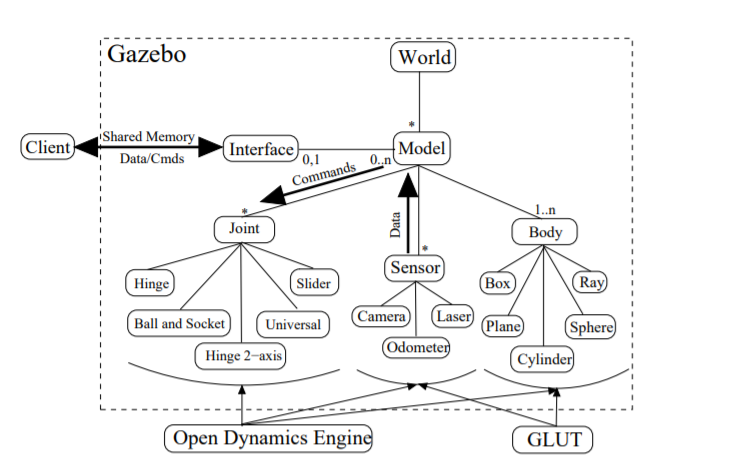
\includegraphics[width=0.99\textwidth]{figures/gazebo-engine.png}
    \caption{Motor de físicas de Gazebo}
    \label{gazebo-physics}
\end{figure}

\begin{figure}[!hbtp]  \centering\noindent
    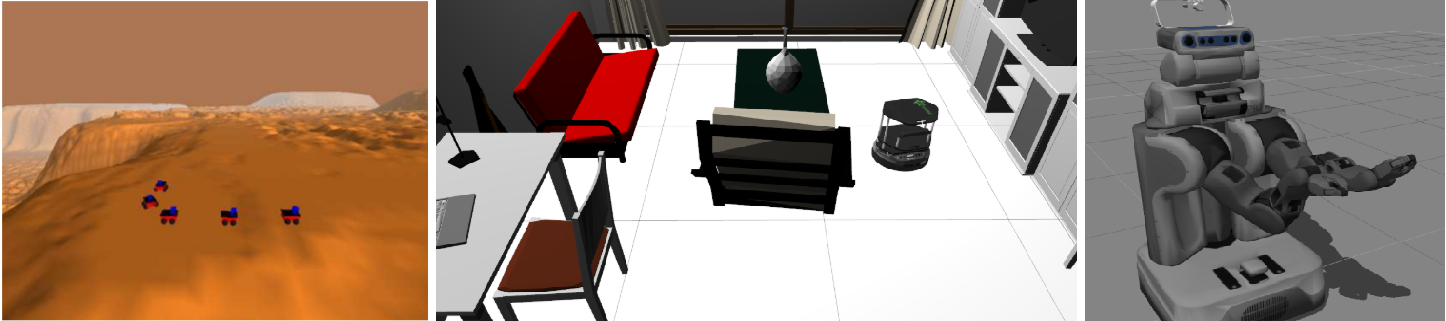
\includegraphics[width=0.99\textwidth]{figures/gazebo-models.png}
    \caption{Modelos de Simulación en Gazebo}
    \label{gazebo-models}
\end{figure}
 
La configuración de mundos 3D con Gazebo se describe en ficheros con extensión ``\textit{.world}'', que son documentos de texto en formato de marcado XML (\textit{Extensible Markup Language}) de documentos, con etiquetas definidas en el lenguaje \textit{Simulation Description Format} (SDF), donde se
recogen todos los elementos del escenario (luz ambiente, propiedades del cielo, sombras, conjunto de modelos, \textit{plugins}, propiedades
físicas y temporales etc.).
 
Aunque la versión 7 de Gazebo incluye un editor de modelos muy básico con el que se pueden crear robots y mundos simples, el simulador acepta la importación de modelos complejos creados con programas de modelado como Blender o Sketchup. A partir del modelo, se especifica un \textit{plugin} asociado al mismo para recoger y publicar la información de los sensores, y para enviar órdenes a los actuadores y dotar al robot simulado de inteligencia e interacción. Es aquí donde se materializa la relación entre el simulador y el sistema de comunicaciones de ROS, que hará las funciones de mediador entre la aplicación y el robot simulado en este caso.

Por último, es importante destacar que cuenta con un cliente web, llamado GzWeb que permite acceder al interfaz de simulación desde un navegador web. Se trata de un cliente con tecnología WebGL que se comunica con un proceso de Gazebo para conseguir que la simulación sea multiplataforma y su acceso no requiera instalación, características ideales para el proyecto.

\section{Biblioteca OpenCV}
En primera instancia, la plataforma que planeábamos diseñar perseguía la ampliación del acceso al campo de la Visión Artificial de la robótica, en tanto que los sensores necesarios (cámaras, ToF, sensores de profundidad) son los más extendidos entre los usuarios de cualquier clase. Es por eso que, aunque la funcionalidad finalmente se extendió para que la plataforma soportase cualquier ámbito de la disciplina robótica, merece una mención especial la tecnología utilizada para el control de los sensores de imagen: las bibliotecas OpenCV\footnote{\url{https://opencv.org/}}.

OpenCV es una librería de código abierto desarrollada inicialmente por Intel y publicada bajo licencia BSD. Incluye gran variedad de herramientas para el tratamiento digital de la imagen y el aprendizaje máquina. Su propósito principal es facilitar la programación de aplicaciones en tiempo real de visión por computador mediante la disposición de módulos de lógica resuelta que implementan alguna técnica de procesamiento o análisis de la imagen (Fig. \ref{opencv}).

\begin{figure}[!hbtp]  \centering\noindent
    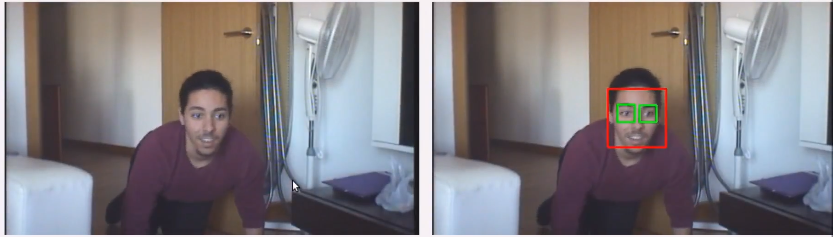
\includegraphics[width=0.99\textwidth]{figures/opencv-face.png}
    \caption{Herramientas de procesado con OpenCV: Segmentación de caras.}
    \label{opencv}
\end{figure}

Se escogió esta librería por ser el estándar en lo relativo a la visión artificial, y se usará tanto para obtener acceso al \textit{hardware} que proporcione la fuente de fotogramas como para utilizarse en la aplicación robótica que se creará para tratar las imágenes.

\section{Lenguajes de Programación: Python, JavaScript}

En cuanto a los lenguajes de programación escogidos para la implementación, se hace necesaria una sub-división en dos ámbitos:

\begin{itemize}
    \item Lenguaje de Aplicación y de Usuario. Es necesario escoger un lenguaje para programar toda la lógica de la aplicación a ofrecer. También se hizo necesario ofrecer un lenguaje al usuario para que aborde su desarrollo robótico.
    \item Lenguaje de Infraestructura. El contexto de tecnologías web en el que se encuentra la ``Ejecución Mixta'' requiere de la elección de un lenguaje que pueda hacer que los distintos agentes colaboren entre sí, principalmente mediante protocolos.
\end{itemize}

Así, el primer lenguaje escogido ha sido Python\footnote{\url{https://www.python.org/}}, como lenguaje de aplicación y usuario. En primer lugar, la elección se debe a la compatibilidad del lenguaje con la infraestructura detallada en este capítulo. Tanto Gazebo como ROS, OpenCV, Jupter y Django ofrecen interfaces Python. Por otro lado están las atractivas características del lenguaje, como sus estructuras de datos integradas de alto nivel, su apariencia intuitiva, y la combinación del tipado y el enlace dinámicos, que hacen al lenguaje idóneo para desarrollar aplicaciones rápidamente. Además, su sintaxis resulta simple y fácil de aprender y enfatiza la legibilidad, lo que a grandes rasgos reduce el costo del mantenimiento del programa. Además fomenta la modularidad del programa y la reutilización de código, lo que lo convierte en un lenguaje de programación muy adecuado para el aprendizaje. Eliminando las peculiaridades que pueden hacer a un lenguaje difícil de tratar, conseguimos que el usuario se centre en su objetivo de carácter robótico y evite los dilemas y contratiempos relacionados con la programación.

En cuanto al lenguaje a usar para la infraestructura de la herramienta, el entorno web hace que la elección de JavaScript\footnote{\url{https://developer.mozilla.org/es/docs/Web/JavaScript}} resulte prácticamente obvia. Desde el 2012, todos los navegadores modernos soportan completamente ECMAScript 5.1\footnote{\url{https://developer.mozilla.org/en-US/docs/Web/JavaScript/Language_Resources}}, el estándar de JavaScript. Por tanto, este lenguaje va a permitir realizar actividades complejas en páginas web, entorno en el que deberá operar la ``Ejecución Mixta'' para aplicaciones robóticas. Este entorno permitirá aprovechar los mecanismos y protocolos de comunicación de Internet para resolver el intercambio de mensajes entre nuestra herramienta, la aplicación robótica, el navegador y el cliente.
	\chapter{Herramienta Web para Enseñanza e Investigación en Visión Artificial y Robótica}
En este capítulo se explica cómo se implementó la idea planteada paso a paso, detallando minuciosamente cómo se alcanzó cada uno de los hitos mencionados y aportando la explicación técnica de los problemas encontrados y las soluciones propuestas.

Se comenzará por describir el diseño de la aplicación robótica a través de la web en cuestión que simplificará el acceso de los usuarios al mundo de la robótica. Se especificarán los puntos desfavorables que desembocan en la necesidad de un mecanismo que resuelva, además de lo anterior, tanto los posibles defectos como la ubicación del peso del cómputo. Para el primer paso se especificará la arquitectura de cada uno de los módulos que componen el servidor remoto y su interfaz de abstracción, para luego desembocar en el diseño y arquitectura finales de la ``Ejecución Mixta'' que aportaran el mencionado cómputo en el cliente y la escalabilidad de la aplicación web.

\section{Servidor Web en Ejecución Remota}

\begin{figure}[!ht]  \centering\noindent
    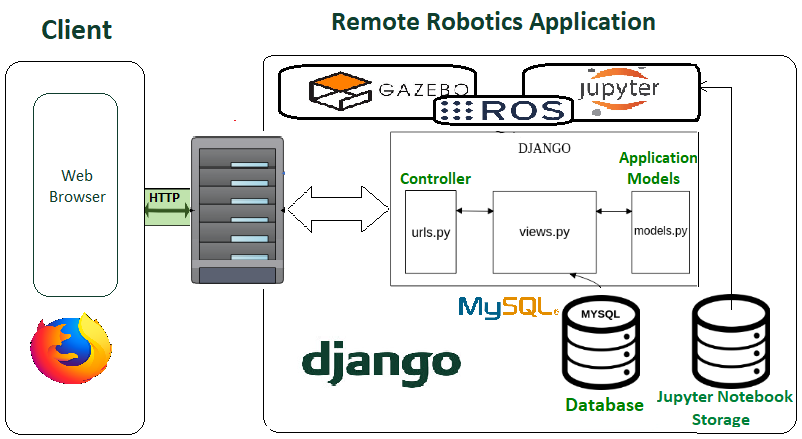
\includegraphics[width=1.20\textwidth,height=8cm]{figures/servidor_remoto_arquitectura.png}
    \caption{Arquitectura del Servidor en Ejecución Remota.}
    \label{remoteexecarch}
\end{figure}

Del mismo modo que no se puede comenzar la casa por el tejado, no podemos empezar con la implementación del mecanismo de la ``Ejecución Mixta'' sin una aplicación robótica a la que conectarla, lo que también servirá para sacar a la luz las carencias o puntos desfavorables relacionados con el servicio web aplicado a la robótica.

\subsection{Diseño del Servidor Web de la Aplicación}

El diseño del contenido prototípico que se quería servir a través de la aplicación web robótica utiliza Django como tecnología de servidor, Jupyter y Gazebo como herramientas en las que se basa la aplicación y sus versiones web para formar el interfaz de usuario y Apache como envoltura para entornos de producción. A fin de ilustrar el funcionamiento y la orientación de la herramienta, decidimos organizar el servicio como una aplicación para el aprendizaje de distintos ámbitos de la robótica por medio de ejercicios con contenido académico.

Como todo servicio web, estará ubicado en un punto físico que resultará siempre remoto al usuario que accede a él, es decir, que se ubica en una red distinta a la del usuario que accede a Internet. Por tanto, este servicio web se basará en el clásico entorno remoto en el que es el lado servidor el que carga con el peso computacional del servicio que ofrece, y el cliente accede a él de manera muy sencilla a través de los motores de búsqueda de su sistema.

Para el diseño de la funcionalidad hemos recurrido a los referentes en aplicaciones web de este tipo, concretamente a la plataforma JdeRobot-Academy, para partir de una organización inicial.

\subsection{Back-end del Servicio}

Como se puede ver en el esquema de arquitectura del servicio web (Fig. \ref{remoteexecarch}), se ha utilizado Django y su gran cantidad de librerías relacionadas con el servicio web y el acceso y gestión de bases de datos para Python para construir el \textit{back-end} o infraestructura del servidor remoto. Como parte de esta estructura de bajo nivel se diseñó una serie de plantillas HTML que actuarán como interfaz de usuario que están alimentadas por variables Python que provienen de las vistas o \textit{views} de Django, las cuales se encargan de la gestión y el procesado de todas las peticiones que los usuarios de la aplicación generan a través del interfaz. La parte más importante de las vistas es la transformación de las peticiones recibidas en este caso en ejercicios concretos de visión artificial y robótica. Para ello es necesario proveer al servidor con ficheros estáticos que harán las funciones de infraestructura de cada ejercicio, con el fin de actuar como capa de abstracción para que el usuario tenga un API sencillo de utilización del ejercicio y las herramientas utilizadas en el \textit{front-end} puedan transformar sus interacciones en acciones concretas sobre el ejercicio y sus agentes simulados o reales.

Cabe destacar que el servicio implementado cuenta con muchos módulos internos encargados de las herramientas básicas de usabilidad y experiencia de usuario, como el inicio de sesión y la gestión de sesiones activas, en las cuales no se va a profundizar al no ser objeto específico de este proyecto.

\begin{figure}[!hbtp]  \centering\noindent
    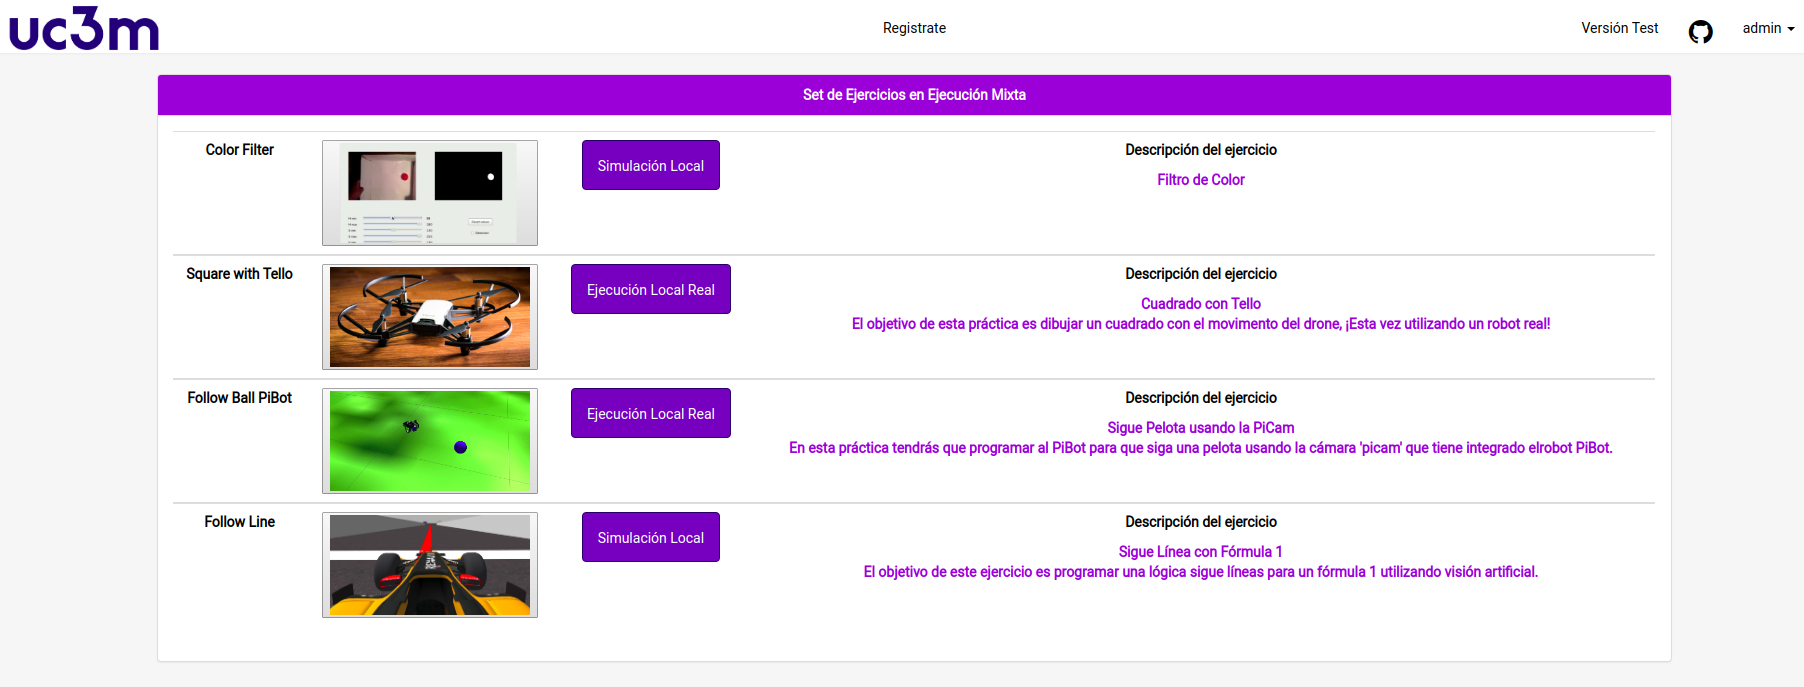
\includegraphics[width=0.99\textwidth]{figures/app_ui.png}
    \caption{UI de la Aplicación en Django}
    \label{appui}
\end{figure}

Como parte del \textit{back-end} encargado del soporte de servicio, se contará tanto con un servidor de Jupyter como con un servidor de Gazebo (\textit{gzserver}) que estarán en constante ejecución durante la solicitud y desarrollo de un ejercicio académico. 

Recordemos que Jupyter es una plataforma de escritorio (requiere instalación) con capacidad de visualización a través de la web. El motor computacional de Jupyter requiere del uso de un \textit{kernel} físico del equipo para llevar a cabo sus funciones, y luego comunica los resultados al interfaz web. Por tanto, el procesado de peticiones cuenta con señales de control que disparan el levantamiento de un servidor remoto de Jupyter (local al servidor web) que será el encargado de ejecutar el código del ejercicio del usuario.  Como se puede ver el contexto inicial es puramente local y supone asumir que el código a ejecutar para el ejercicio robótico proviene de la misma máquina que lo sirve, y por tanto se va a encargar de todo el cómputo. 

Por otro lado, la simulación a través de Gazebo sucede en un escenario análogo al de Jupyter, ya que también se trata de una aplicación de escritorio con interfaz web. Por tanto, también ha de levantarse un servidor de Gazebo que atienda a las peticiones de simulación. Todo lo anterior supone un grave problema atendiendo a la escalabilidad y la eficiencia computacional, dado que la conjunción de varios usuarios simultáneos generaría una carga de cómputo no asumible para el servicio, que para dar soporte a cada uno debería levantar una instancia de ambas aplicaciones.

En cuanto a la conexión entre ambas partes, simulador y código, utilizamos ROS como \textit{middleware} de comunicaciones dada su fácil integración con Gazebo y el lenguaje Python. Esto permite construir una aplicación completa y autocontenida asociada al código del ejercicio que creará el mecanismo de inter-comunicación a través de mensajes de ROS (\textit{ROS Messages}) que se intercambian por canales o \textit{topics} de publicación y suscripción de información (Listing. 4.1). De esta manera los resultados de las instrucciones que el usuario coloque en su código se reflejan en la simulación.

\begin{lstlisting}[language=bash, caption=Topics de ROS asociados a los Canales de Comunicación Internos]
~$ rostopic list
/F1ROS/cameraL/camera_info
/F1ROS/cameraL/image_raw
/F1ROS/cameraL/parameter_descriptions
/F1ROS/cameraL/parameter_updates
/F1ROS/cmd_vel
/F1ROS/odom
/clock
/gazebo/link_states
/gazebo/model_states
/gazebo/parameter_descriptions
/gazebo/parameter_updates
/gazebo/set_link_state
/gazebo/set_model_state
/rosout
/rosout_agg
/tf
\end{lstlisting}

De nuevo, todo este mecanismo añade demasiada carga al lado servidor, que empieza a requerir soporte computacional adicional para dar servicio, como granjas de ordenadores de soporte o procesadores adicionales. Además, cabe destacar también que el uso de un servicio web remoto como el descrito está muy limitado en cuanto a la variedad de robots soportados. Se ha de tener en cuenta que, por ejemplo en el uso de una cámara, el ejercicio que se construya estará supeditado al tipo de \textit{hardware} del que se disponga en el lado servidor, al entorno de servicio en el que la cámara será estática (lo que limita la riqueza de ejercicios que se pueden construir al estar siempre enfocando al mismo entorno), y en todo caso imposibilita el empleo de los robots de los que los usuarios puedan disponer.

Para poner este servicio en producción y que los usuarios puedan acceder a él es necesario el empaquetamiento de toda la estructura en una envoltura de servidor HTTP dado que Django no ofrece por sí mismo este soporte. La tecnología Apache interviene para cumplir esta función. Se trata simplemente de una capa de servidor HTTP orientado a dar un formato correcto a todas las peticiones generadas desde el servicio web y destinadas a él para que puedan viajar por Internet sin percances. Aporta también mecanismos extra de seguridad para proteger el servicio frente a las intrusiones y permite configurar una capa de TLS a través del protocolo SSL y el uso de certificados de encriptación de información.

Todo ello se refleja en los ficheros de configuración de servicio de Apache, compuestos por directivas que indican el tipo de cabeceras HTTP que deben llevar los mensajes, los \textit{endpoints} donde la aplicación web espera a recibir peticiones, la ubicación de los ficheros estáticos y la configuración básica de seguridad, permisos de actuación y servicio.

\subsection{Front-end de la Aplicación}

Una vez preparada la estructura básica de gestión de peticiones, se construye encima de la misma la capa de usuario o \textit{front-end} de la aplicación para los ejercicios. El agente encargado de disponer el interfaz de usuario será el navegador web del cliente. Este interfaz se basa en un cuadernillo de Jupyter que permita al usuario, desde el navegador, visualizar el resultado de una ejecución de código Python. Dado que los ejercicios emplearán algún tipo de robot o sensor, también se incluye en la interfaz una sección de simulación con GzWeb o divisiones auxiliares que contendrán la información necesaria para que el usuario pueda depurar y resolver el ejercicio, como visualizadores de imágenes de una cámara.

Así, la interacción del usuario se realiza sobre un \textit{Notebook} de Jupyter almacenado en el servidor cuya función es actuar como interfaz de edición de la aplicación (IDE), que enviará mensajes al \textit{kernel} del servidor para que compute.

\begin{figure}[!hbtp]  \centering\noindent
    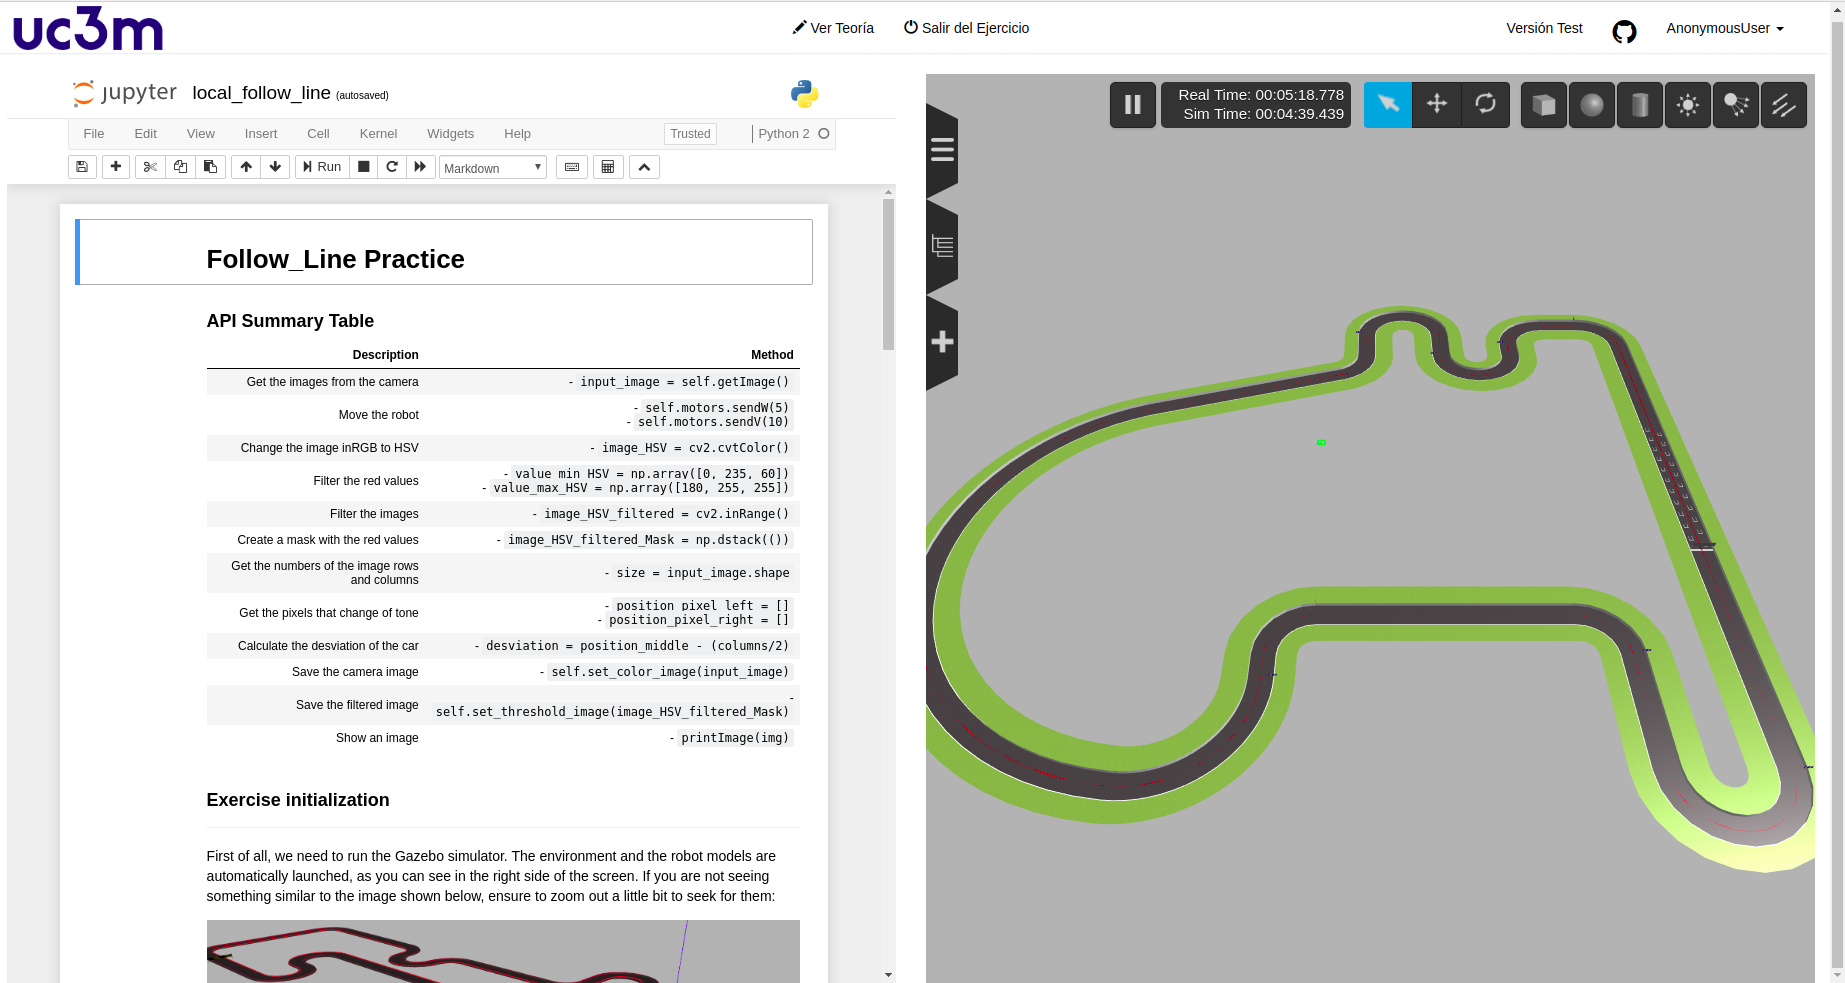
\includegraphics[width=0.99\textwidth]{figures/ui_simulation.png}
    \caption{UI de Simulación de la Aplicación}
    \label{simui}
\end{figure}

Se puede ver que el cliente web no asume ninguna carga de procesamiento, sino que sólo cuenta con un navegador que en todo momento solicita la visualización de varias aplicaciones que están corriendo coordinadas en el lado del servidor web.

\section{``Ejecución Mixta''}

\begin{figure}[!ht]  \centering\noindent
    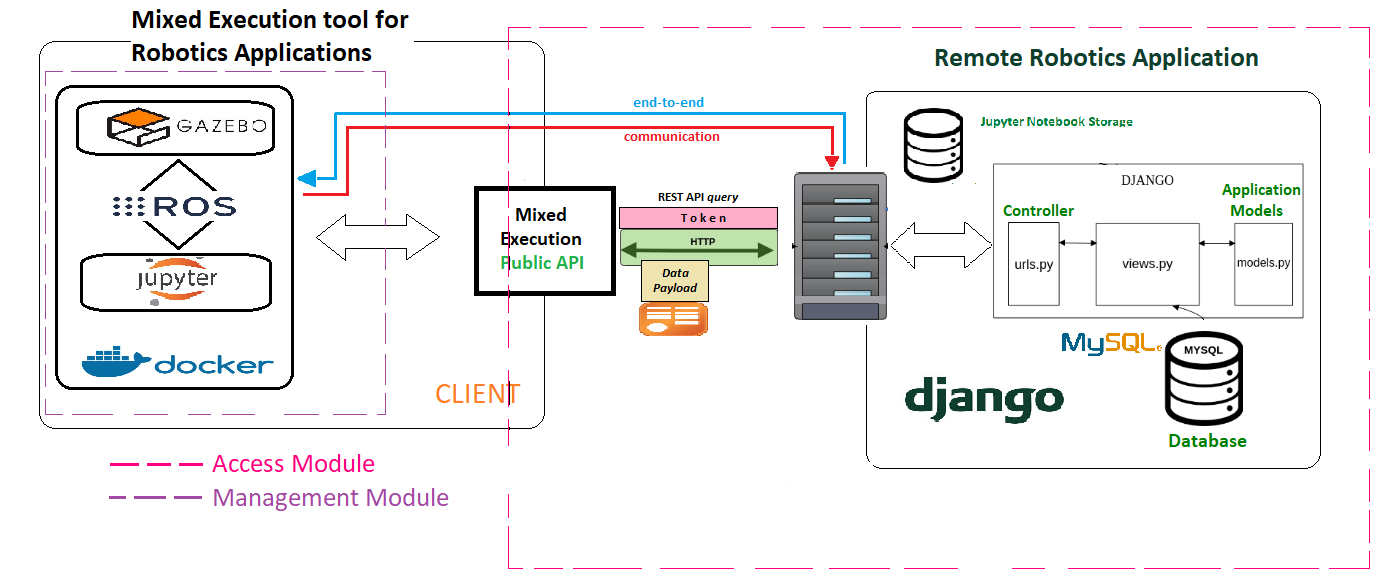
\includegraphics[width=1.20\textwidth,height=9cm]{figures/ejecucion-mixta-infograma.png}
    \caption{Arquitectura de la Ejecución Mixta para Aplicaciones de Robótica.}
    \label{mixedexecarch}
\end{figure}

En este punto, disponemos de una versión completamente remota del servicio de aprendizaje y docencia que se quiere construir. Se han relatado los problemas derivados de este tipo de servicio, y se puede ver claramente como no encajan con las características deseadas para la herramienta robótica objeto de esta tesis. Por tanto, y tras la investigación correspondiente, se procedió a la implementación de un \textit{local runtime}, es decir, de un entorno de ejecución utilizando un \textit{kernel} local al cliente, en comunicación constante con la aplicación web remota. Había que desarrollar un servidor remoto que contuviese la aplicación y el modelo de ejercicio creado y que, ante una nueva petición del ejercicio, estableciese una comunicación fluida con el \textit{kernel} del cliente para coordinar la ejecución en su \textit{hardware}, por medio del lanzamiento del servidor de ``Ejecución Mixta'' en su máquina. 

Partiendo del básico servidor web en Django (Fig. \ref{appstructure}), descrito anteriormente, con capacidad para atender a un cliente que solicitase un ejercicio por medio de un click en el interfaz web, se colocó la arquitectura de ``Ejecución Mixta'' debajo del botón sobre el que el usuario hace click para entrar al ejercicio que resolverá el mecanismo de enlazado y comunicación para disponer el entorno mixto.

Como se puede ver en la imagen (Fig. \ref{simui}) de la interfaz que ofrece el servidor web a su cliente, es necesario para el correcto funcionamiento de la herramienta que el receptor principal de los mensajes de ``Ejecución Mixta'' sea Jupyter, y por tanto también tiene sentido que se use como editor de código. Tras la conexión HTTPS con el servidor web, lo primero que debe hacer el cliente es especificar su dirección IP y el puerto en que está corriendo el servidor de Jupyter en su máquina dado que, como ya es sabido, es necesario que este escuche físicamente en una máquina para poder acceder al \textit{hardware} de la misma. De esta manera se puede establecer fácilmente un puente que permita que el servidor acceda a los datos generados por Jupyter desde un punto remoto, y los ofrezca al usuario como parte del interfaz, a través de un mecanismo de paso de mensajes de actualización periódicos. Esto requiere hacer unos cambios sobre el servidor provisto por el proyecto Jupyter con el fin de abrir el acceso a él desde el exterior, no sin antes establecer los correspondientes métodos de seguridad. Se profundizó en la arquitectura de servicio de Jupyter para poder adaptar su funcionamiento a nuestras necesidades.

Se infiere la necesidad de una especie de servidor en el lado cliente web que difunda la información de una ejecución local a quien la solicite. Este es precisamente el servidor de ``Ejecución Mixta''. Para lograr la ejecución del código del cliente localmente a través de órdenes generadas en el interfaz ofrecido por un servidor remoto, se hace indispensable proveer al servidor de ``Ejecución Mixta'', concretamente al \textit{kernel} de Jupyter, del código asociado al ejercicio para que pueda ejecutarlo, y también de un mecanismo de retorno de los resultados para que el servicio web pueda reflejarlos en el interfaz de visualización de usuario. Aquí comienza el mecanismo de establecimiento y supervisión de la conexión HTTPS que llevará a cabo la denominada Capa de Comunicación. La conexión con Jupyter puede hacerse de manera sencilla mediante el envío de un simple mensaje bajo el método OPTIONS, al que el servidor responderá con toda la información que necesitamos para el establecimiento de la conexión a través de cabeceras HTTP, entre ellas el \textit{token} de autenticación de Jupyter, los métodos y tipos de contenido que se aceptan, y el código CSRF\footnote{\href{https://www.geeksforgeeks.org/what-is-cross-site-request-forgery-csrf/}{What is CSRF and how to prevent it?}} necesario para enviar información al servidor de Jupyter desde otros puntos.

Al obtenerse esta información se ha de disponer un canal entre el servicio web remoto y el servicio de ejecución local, para lo cual no existen soluciones. Estudiamos el mecanismo de comunicación de la plataforma, que emplea principalmente el protocolo ZeroMQ\footnote{\url{https://zeromq.org/}} o 0MQ para el intercambio asíncrono de mensajes \textit{N-a-N} a través de la web. Esto nos proporciona, además de una plantilla para los tipos de mensajes que debemos enviar al \textit{kernel} de Jupyter, una idea bastante fiel del proceso que desencadena cada órden o petición que se le hace al servidor de Jupyter. También se utilizó \textit{sniffers}\footnote{\href{https://www.wireshark.org/\#1398253364-1-69}{Wireshark Sniffer}} para monitorizar el funcionamiento local de Jupyter (Fig. \ref{wireshark}). Este paso fue vital para comprender el procedimiento que debíamos seguir para iniciar una sesión de Jupyter completa y válida.

\begin{figure}[!hp]  \centering\noindent
    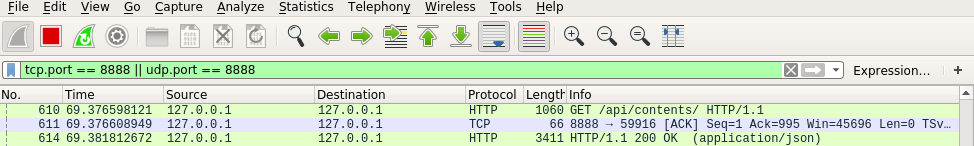
\includegraphics[width=0.99\textwidth]{figures/wireshark.png}
    \caption{Capura de Paquetes del Mecanismo de Comunicación de Jupyter}
    \label{wireshark}
\end{figure}

Por tanto tras el establecimiento, se puede comenzar con el intercambio de mensajes 0MQ. Aprovecharemos el REST API que ofrece Jupyter para la comunicación con el \textit{kernel} en tanto que este \textit{RESTfull Service}\footnote{\href{https://docs.oracle.com/javaee/6/tutorial/doc/gijqy.html}{What is a RESTfull Service?}} ofrece todo lo necesario para enviarle ficheros de código, órdenes de ejecución, órdenes de control (reinicio, apagado, encendido, pausa, cambio de lenguaje, limpieza de salidas, etc.) (Fig. \ref{jupyter_rest_api}) y, en general, lo necesario para facilitar el uso de la plataforma a través de la web. Por tanto, por el canal de ``Ejecución Mixta'' estaríamos enviando, principalmente, mensajes HTTP sobre una capa de TLS con datos de tipo 0MQ en el cuerpo, destinados a Jupyter que viajan por Internet.

\begin{figure}[!ht]  \centering\noindent
    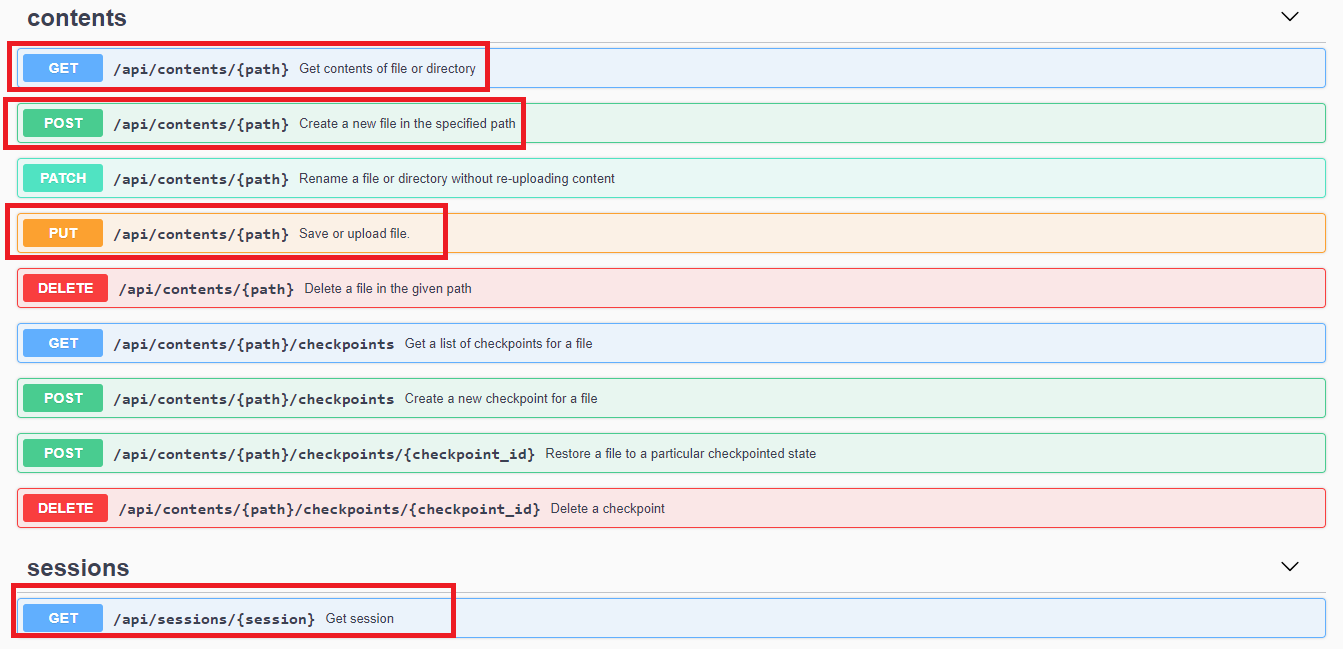
\includegraphics[width=0.99\textwidth]{figures/jupyter_rest_api.png}
    \caption{REST API de Jupyter}
    \label{jupyter_rest_api}
\end{figure}

En base al conocimiento obtenido del motor de comunicación de Jupyter, seleccionamos aquellos métodos del REST API que necesitaríamos, marcados en la imagen superior. Se muestra a continuación un ejemplo del mensaje que se enviaría al servidor de Jupyter para hacer llegar el código al \textit{kernel} encargado de un cuadernillo concreto:

\lstset{
   language=JavaScript,
   backgroundcolor=\color{lightgray},
   extendedchars=true,
   basicstyle=\footnotesize\ttfamily,
   showstringspaces=false,
   showspaces=false,
   numbers=left,
   numberstyle=\footnotesize,
   numbersep=9pt,
   tabsize=2,
   breaklines=true,
   showtabs=false,
   captionpos=b
}
\begin{minipage}{\linewidth}
\begin{lstlisting}[caption=Formato de Mensajes de ``Ejecución Mixta'']
const url = 'http://'+_ip+':'+_port+'/api/contents/' + nbname;
const data_put = ' {"type": "notebook",
                    "format": "json",
                    "content": ' + nbcontent + '} ';
const message = {
        headers:{'Content-Type':'application/json',
                 //'Authorization': 'token ' + _token,
                },
        body:data_put,
        method:"PUT"
};
\end{lstlisting}
\end{minipage}

donde cada variable que aparece en el mensaje (\textit{\_ip, \_port, nbname,\_token, nbcontent}) sería establecida por el servidor web y contendría la dirección del servidor Jupyter y el contenido y nombre del cuadernillo que queremos enviar, almacenado en el servidor remoto y solicitado por el usuario web. El formato de todos los mensajes es similar, en tanto que se trata de peticiones HTTP como se puede ver en la constante \textit{message} con el formato de cuerpo 0MQ que se refleja en la constante \textit{data\_put}. Este tipo de mensajes, con su respectiva codificación, constituye el tipo de mensajes a intercambiar por la herramienta ``Ejecución Mixta'' para el establecimiento y envío iniciales.

El proceso de comunicación con Jupyter comenzaría por el establecimiento de la conexión, donde se crea una sesión de ejecución, continuaría con el envío del código del cuadernillo y de cada fichero de código de aplicación auxiliar que necesite el ejercicio, para acabar con una orden de inicio del \textit{kernel} del lenguaje adecuado encargado de la ejecución, que se montará sobre un núcleo latente en el sistema del cliente web. La utilización de direcciones IP públicas, el protocolo HTTP (estándar de Internet) que utiliza por defecto el puerto 8080 (puerto de Internet, abierto a mensajes transportados sobre TCP o UDP por la red, con cualquier origen) que puede atravesar \textit{firewalls} y resolver conexiones sea cual sea el dominio público, y el \textit{token} de autorización embebido en los mensajes garantizan la conectividad y la integridad de la sesión de Jupyter, así cómo el funcionamiento entre sistemas bajo distintas redes o sub-redes de la misma red.

En este punto del desarrollo, hemos superado el principal obstáculo de la ``Ejecución Mixta'' e implementado un mecanismo capaz de ejecutar código entre redes, con actualización de los resultados en tiempo real en ambos lados servidor  y cliente web. Se completa así el primer ciclo de trabajo, no sin antes realizar los tests convenientes de funcionamiento y desempeño y el análisis de los resultados. La herramienta ya es capaz de conectar un código remoto (aplicación robótica) con un ``robot'' local (cámara). Esto sortea tanto el obstáculo de desbordamiento de cómputo en el lado servidor, pues es ahora el cliente el que carga con la mayor parte del peso computacional, como la limitación de \textit{hardware} conectable a la aplicación web, ya que ahora el cliente puede emplear su propia cámara o incluso sus propios robots en los ejercicios, accesibles desde su máquina y su red, pero no desde el exterior.

Sin embargo, la dependencia de este servidor de ejecución local supone para el cliente la instalación de todas las herramientas, tanto Jupyter como Gazebo y ROS, para mantener el soporte del servicio web de manera local. Las ventajas obtenidas se ven empañadas por una serie de desventajas claras entre las que se encuentran principalmente el proceso de instalación (tedioso, requiere espacio de disco del cliente) y la compleja organización inter-plataforma necesaria para comunicar las herramientas locales. El usuario necesitaría un programa encargado de cumplir estas funciones, lo cual desmontaría el servicio web.

La alternativa diseñada pasa por utilizar contenedores Docker (lo cual cambiará sustancialmente el mecanismo de comunicación), sobre los que se puede construir una arquitectura de módulos que cuente con un mecanismo interno de comunicación entre plataformas y otro externo que se comunique con la aplicación remota. Por medio de Docker se puede conservar la funcionalidad previa, evitar el proceso de instalación y organizar de alguna manera la comunicación entre un agente remoto y los servicios locales al cliente de la ``Ejecución Mixta''.

Hubo que estudiar el motor de Docker y su funcionamiento para crear un \textit{DockerFile} con instrucciones en lenguaje SHELL para virtualizar una distribución Ubuntu con todas las herramientas y aplicaciones auxiliares involucradas en la ``Ejecución Mixta'', para que utilizar la herramienta resultase tan fácil como descargar la imagen Docker y levantar el contenedor. Utilizar un contenedor Docker para empaquetar los procesos necesarios e incluir seguridad supone añadir complejidad el mecanismo de comunicación, en tanto que Docker levanta su propia sub-red dentro de la red del cliente, lo que nos deja una intratable sub-red dentro de una red distinta desde el punto de vista del servidor web. Se replanteó el mecanismo de comunicación para que utilizase el navegador del cliente web como intermediario entre el usuario y la aplicación robótica en lugar de la previa comunicación punto a punto, el cual sí que tiene conectividad directa con una sub-red de su propia red. Por tanto, el servidor web abre ahora una comunicación con el \textit{browser} del cliente en lugar de directamente con el servidor Jupyter, y éste actúa como \textit{proxy} reenviando cada mensaje donde corresponde a través de una secuenciación programada en código JavaScript, de manera que tanto de cara al cliente como al servidor web, la comunicación sigue siendo la misma que en el paso anterior, esta vez con un origen o destinatario distinto. Simplemente se trata de añadir la lógica del \textit{proxy} para que viaje con la aplicación que se sirve al usuario web. El navegador ya utiliza protocolos como STUN o ICE que permiten descubrir e interaccionar con ambas partes del mecanismo. Así, los mensajes reenviados por el navegador serán recibidos por un módulo secuenciador de ``Ejecución Mixta'', que procesará la información que llega para orquestar el correcto inicio del entorno y los agentes, traduciendo las órdenes JavaScript iniciales a comandos de lanzamiento (Listing. 4.3) y entregando las órdenes de ejecución a quien corresponda (Listing. 4.4).

\begin{lstlisting}[language=bash, caption=Código de Inicio del Secuenciador]
#!/bin/bash

rm -rf /tmp/.X0-lock

Xvfb -shmem -screen 0 1280x1024x24 &

source /opt/jderobot/setup.bash
source /opt/ros/kinetic/setup.bash
source /opt/jderobot/share/jderobot/gazebo/gazebo-assets-setup.sh
export PYTHONPATH=$PYTHONPATH:/home/jderobot/.exercises

cd ~/gzweb
npm start &

cd ~/volume/user/exercise

jupyter nbextension enable hide_input/main --user
jupyter nbextension enable init_cell/main --user
jupyter notebook --ip=0.0.0.0 --allow-root &

cd ~

EXTENSION=`echo "$1" | cut -d'.' -f2`
if [ $EXTENSION = "world" ]
  then
    roscore &
fi

if ! [ -z "$2" ]
  then
    python ~/referees/$2 &
fi

if ! [ -z "$1" ]
  then
    EXTENSION=`echo "$1" | cut -d'.' -f2`
    if [ $EXTENSION = "launch" ]
      then
        roslaunch /opt/jderobot/share/jderobot/gazebo/launch/$1
    else
        rosrun gazebo_ros gazebo /opt/jderobot/share/jderobot/gazebo/worlds/$1
    fi
else
    tail -f /dev/null
fi
\end{lstlisting}
\begin{lstlisting}[language=bash, caption=Reenvío de Mensajes]
[I 11:51:09.187 NotebookApp] Saving file at /thumbnail_follow_line.png
[Gazebo] Sat Jan 11 2020 11:51:09 GMT+0000 (Coordinated Universal Time) Received Message: {"op":"advertise","id":"advertise:~/heartbeat:14","type":"heartbeat","topic":"~/heartbeat"} from http://127.0.0.1:8080 ::ffff:172.17.0.1
[Python Process] Sat Jan 11 2020 11:51:09 GMT+0000 (Coordinated Universal Time) Received Message: {"op":"publish","id":"publish:~/heartbeat:15","topic":"~/heartbeat","msg":{"alive":1}} from http://127.0.0.1:8080 ::ffff:172.17.0.1
[I 11:51:11.758 NotebookApp] 302 GET /notebooks/world.png (172.17.0.1) 0.95ms
[I 11:51:11.847 NotebookApp] Adapting to protocol v5.1 for kernel 368a1e46-acc2-4976-acf3-25528ae77d77
\end{lstlisting}

El API de inicio de la ``Ejecución Mixta'' fue enriquecido con la aparición de los parámetros característicos de Docker que permiten crear un puente seguro entre un elemento virtualizado y su homólogo en la máquina anfitrión. Un ejemplo de esto es el mecanismo de acceso a la cámara integrada en el sistema cliente desde el interior de un contenedor Docker, resuelto con el mapeo \textit{-v /dev/video0:/dev/video0}, o la redirección de interfaces de escucha del sistema a sus correspondientes dentro del contenedor (\textit{-p 8888:8888 -p 8889:8889 -p 8080:8080}).

El contenedor de ``Ejecución Mixta'' ejecuta tanto la lógica como la simulación y aplicaciones auxiliares como \textit{plugins} o \textit{drivers} robóticos que actúen como controlador del dispositivo \textit{hardware} real. El mecanismo interno de comunicaciones a través de ROS pasa ahora por el secuenciador del denominado Módulo de Gestión, configurado para actuar de intermediario (Listing. 4.5), que reenvia los mensajes a quien corresponde y elabora una respuesta destinada al servicio web remoto a través de un canal WebSockets, envuelto con una capa HTTPS para que éste último lo procese (Fig. \ref{mixedexecarch}).
\begin{minted}[
    gobble=4,
    frame=single,
    linenos
  ]{yaml}
    Camera:                               # follow_line.yml
      Topic: "/F1ROS/cameraL/image_raw" 
      Name: follow_line_camera
    Motors:
      Topic: "/F1ROS/cmd_vel"
      Name: follow_line_motors
      MaxV: 40
      MaxW: 2
    Websockets:
      Host: 0.0.0.0 
      Port: 9002
      SSL: False
      Cert: '/etc/certs/fullchain1.pem' 
      Key: '/etc/certs/privkey1.pem'
\end{minted}
\begin{lstlisting}[caption=Configuración de Canales Inernos del Secuenciador en formato YAML]
\end{lstlisting}

La inclusión de la ``Ejecución Mixta'' ya no supone ninguna carga de cómputo para el lado servidor de la aplicación web y queda eliminado el proceso de instalación, dado que todas las dependencias están agrupadas en el contenedor. Lanzar la ``Ejecución Mixta'' pasa ahora por utilizar el API de Docker de control de contenedores, que pondrá en marcha todos los sub-sistemas necesarios para el funcionamiento de la aplicación robótica y los dejará disponibles para su consulta desde el exterior, por parte del servidor remoto a través del secuenciador o \textit{proxy} web. Así, la aplicación puede enviar cualquier tipo de orden de ejecución en formato Python al servidor de Jupyter, que materializará esa orden en el simulador Gazebo a través de los canales ROS o, incluso, en el robot o sensor real conectado al sistema del cliente. La aplicación robótica le indicará al secuenciador qué sub-procesos necesita para el funcionamiento de un ejercicio robótico concreto.

Para implementar el soporte de simulación, se diseñó un sistema de configuración que permite indicar los elementos, robots y características que debe tener la escena simulada a través de Gazebo (Fig. \ref{gzworld}), haciendo uso de ficheros de extensión \textit{.world} o \textit{.launch}, siendo los primeros un subconjunto del lenguaje de marcado XML que indica los agentes involucrados en la simulación (Listing. 4.7), y el segundo un configurador inteligente que permite lanzar, además del mundo de simulación, una serie de nodos que se puedan necesitar para controlar por ejemplo las interfaces de un determinado robot (Listing. 4.6). 

\begin{figure}[!hbtp]  \centering\noindent
    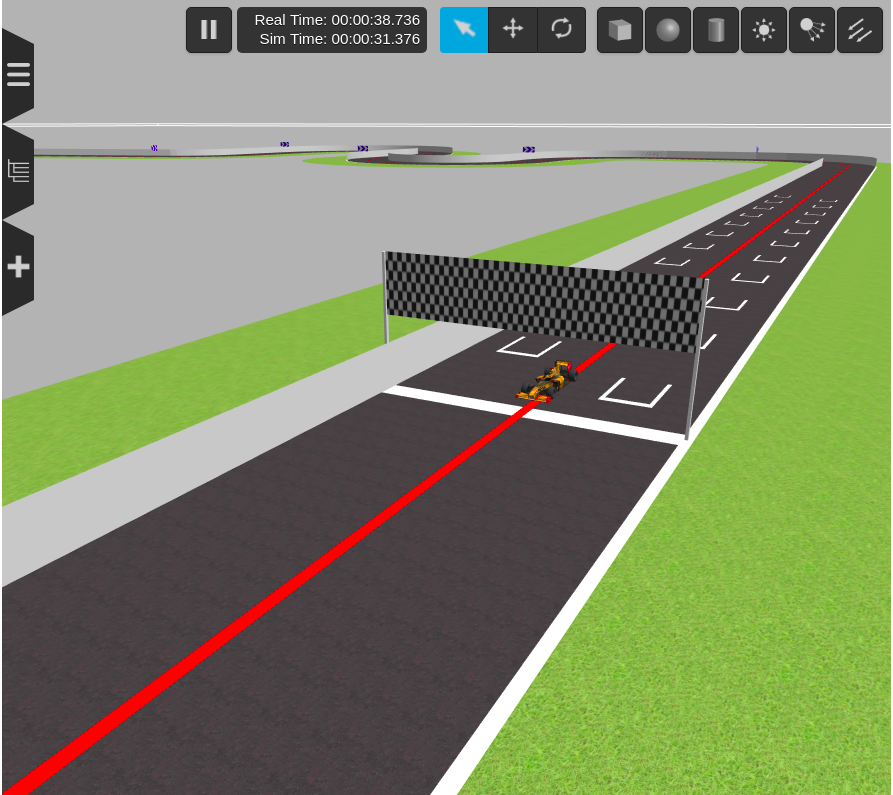
\includegraphics[width=0.9\textwidth]{figures/world_gazebo.png}
    \caption{Escenario de Simulación}
    \label{gzworld}
\end{figure}

\begin{lstlisting}[language=XML, caption=Configuración de Lanzamiento de Simulaciones]
<?xml version="1.0" encoding="UTF-8"?>
<launch>
  <!-- We resume the logic in empty_world.launch, changing only the name of the world to be launched -->
  <include file="$(find gazebo_ros)/launch/empty_world.launch">
    <arg name="world_name" value="f1_1_simplecircuit.world"/> <!-- Note: the world_name is with respect to GAZEBO_RESOURCE_PATH environmental variable -->
    <arg name="paused" value="false"/>
    <arg name="use_sim_time" value="true"/>
    <arg name="gui" value="true"/>
    <arg name="headless" value="false"/>
    <arg name="debug" value="false"/>
    <arg name="verbose" default="false"/>
  </include>  
</launch>
\end{lstlisting}

\begin{lstlisting}[language=XML, caption=Configuración de Lanzamiento de Simulaciones]
<?xml version="1.0" ?>
<sdf version="1.5">
  <world name="default">
    <scene>
      <grid>false</grid>
    </scene>
    <!-- A global light source -->
    <include>
      <uri>model://sun</uri>
    </include>
    <include>
	    <uri>model://pista_simple</uri>
	    <pose>0 0 0 0 0 0</pose>
    </include>
    <include>
      <uri>model://f1_renault</uri>
      <pose>53.462 -10.734 0.004 0 0 -1.57</pose>
    </include>
    <scene>
        <sky>
            <clouds>
                <speed>12</speed>
            </clouds>
        </sky>
     </scene>
  </world>
</sdf>
\end{lstlisting}

Con ello, al lanzar la herramienta se indicará qué fichero de configuración se quiere usar a través de instrucciones del API de ``Ejecución Mixta'', que se ocupará de levantar tanto la simulación como la red de comunicación interna basada en ROS como se puede ver en el \textit{snippet} de código inferior (Listing. 4.8), y la capa de abstracción que permite al usuario programar su robot y acceder a toda la funcionalidad mientras se materializan los cambios en el simulador.

\begin{minted}[
    gobble=4,
    frame=single,
    linenos
  ]{python}
    class ListenerCamera:
        def __init__(self, topic):
            
            self.topic = topic
            self.data = Image()
    
        # [...]
    
        def start (self):
     
            self.sub = rospy.Subscriber(self.topic, ImageROS,
                                        self.__callback)
    
    class PublisherMotors:
     
        def __init__(self, topic, maxV, maxW):
    
            self.maxW = maxW
            self.maxV = maxV
    
            self.topic = topic
            self.data = CMDVel()
            self.pub = rospy.Publisher(self.topic,
                                       Twist,
                                       queue_size=1)
            rospy.init_node("FollowLineF1")
    
        # [...]
    
        def publish (self):
    
            self.lock.acquire()
            tw = cmdvel2Twist(self.data)
            self.lock.release()
            self.pub.publish(tw)
    
    class FollowLine():
        
        def __init__(self):
            cfg = readConfig()
    
            cameraTopic = cfg["Camera"]["Topic"]
            motorsTopic = cfg["Motors"]["Topic"]
            maxv = cfg["Motors"]["MaxV"]
            maxw = cfg["Motors"]["MaxW"]
    
            self.camera = ListenerCamera(cameraTopic)
            self.motors = PublisherMotors(motorsTopic, maxv,
                                          maxw)
    
            # [...]
\end{minted}
\begin{lstlisting}[caption=Creación de la Red Interna de Comunicación]
\end{lstlisting}

Dada la filosofía modular interconectada que se había diseñado hasta este momento, el enfoque para el caso de querer controlar un robot real desde el lado cliente pasaba sencillamente por crear su controlador, e incluirlo como aplicación auxiliar lanzada dentro de la herramienta y orquestada como un módulo más por el secuenciador.

Se tiene una herramienta que actúa como \textit{middleware} entre un servicio web remoto y una serie de aplicaciones locales al cliente capaz de lanzar un proceso de ejecución compartida con una serie de ventajas claras, entre las que se encuentran el uso de robots reales del cliente, el bajo cómputo en el lado servidor web, la versatilidad de contenidos que se puede crear para la aplicación y, sobre todo, la accesibilidad a las aplicaciones robóticas.

\subsection{Diseño e Infraestructura de la herramienta}

En esta sección abordaremos el diseño final de las distintas capas que componen la herramienta y la jerarquía establecida. Se puede ver en el infograma (Fig. \ref{mixedexecarch}) que la solución ideada para la ``Ejecución Mixta'' se divide claramente en dos módulos, cada uno sub-dividido a su vez en una serie de capas encargadas de una parte específica del proceso:

\begin{itemize}
    \item [\textbullet] El primero de ellos es el \textbf{módulo de acceso}. Este módulo será el encargado de dirigir la comunicación entre el lado servidor y el lado cliente de la aplicación para que se produzca la ``Ejecución Mixta''. Organizará ambas partes y actuará como un secuenciador que decidirá en cada momento quién lleva el peso de la comunicación. Su propósito principal será el de garantizar el acceso a la herramienta.
    \item [\textbullet] El otro es el \textbf{módulo de gestión}. Estará recubierto por un API público que permitirá a las aplicaciones web externas realizar la conexión y aprovechar las funciones de ``Ejecución Mixta'' para ofrecer un servicio. Será el encargado de redirigir cada petición y respuesta de la aplicación al proceso que corresponda de forma segura, dentro de la ejecución del cliente.
\end{itemize}

Dada la clara distinción entre las distintas sub-tareas que realiza cada módulo, consideramos adecuado bajar otro escalón en cuanto a la arquitectura, y dividir cada módulo en capas encargadas de tareas sencillas, sobre las que se pudiese construir de manera modular. 

\subsubsection{Capa de Aplicación}

\begin{figure}[!hbtp]  \centering\noindent
    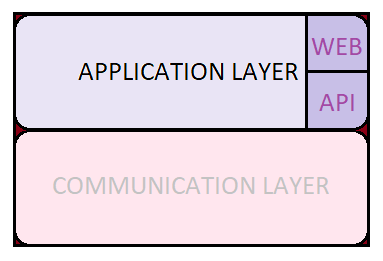
\includegraphics[width=0.6\textwidth]{figures/layer4.png}
    \caption{Módulo de Acceso: Capa de Aplicación}
    \label{layer4}
\end{figure}

La capa de aplicación tendrá la tarea específica de emparejar la funcionalidad que ofrece la aplicación remota como servicio con la información que necesita de la ejecución en el lado cliente para dar soporte a dicha funcionalidad. Requerirá de la intervención de dos agentes para cumplir su tarea:

\begin{itemize}
    \item [--] Será necesario que la aplicación robótica que se ofrece a través de la web que quiere beneficiarse de la ``Ejecución Mixta'' inicie la conexión con el cliente remoto, en calidad de cliente de ``Ejecución Mixta''. Esto es así dada la naturaleza de la información a la que más tarde pedirá acceso, la cual se genera completamente en el cliente durante la ejecución y pondrá a disposición de quien la solicite. El cliente de la aplicación web hace las funciones de servidor de la herramienta, ya que está pensada para ser colocada en el lado del cliente web.
    \item [--] Con la conexión iniciada, esta capa debe solicitar la información que necesite al servidor de ``Ejecución Mixta'', en tiempo de ejecución, para que la aplicación funcione como se espera. Esta solicitud se realizará a través del API de ``Ejecución Mixta''.
\end{itemize}

Así, el mecanismo completo de la capa de aplicación comenzará por establecer la conexión con la herramienta, utilizando uno o varios \textit{endpoints} en función de los canales de comunicación que se quiera establecer para recopilar la información necesaria y generará un comando específico para configurar en la herramienta el tipo de enlace que se requiere y el conjunto de herramientas que se necesita para la ejecución.

\begin{lstlisting}[language=bash, caption=Comando de configuración de Ejecución Mixta]

mkdir -p /tmp/siguelineaIR/ && docker run --rm -e DISPLAY=:0
-e JDEROBOT_SIMULATION_TYPE=REMOTE --entrypoint 
/entrypoint_mixed_execution.sh -v 
/tmp/siguelineaIR:/home/jderobot/volume/user/exercise:rw 
-p 8888:8888 -p 8080:8080 -p 9001:9001 -p 9002:9002 
-it tfmdocker/local:dev f1_1_simplecircuit.launch

\end{lstlisting}

\subsubsection{Capa de Comunicación}

\begin{figure}[!hbtp]  \centering\noindent
    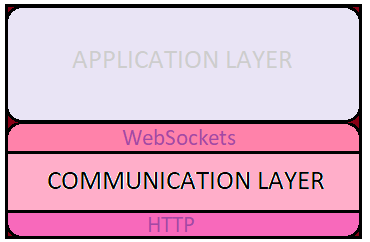
\includegraphics[width=0.6\textwidth]{figures/layer3.png}
    \caption{Módulo de Acceso: Capa de Comunicación}
    \label{layer3}
\end{figure}

Encargada del establecimiento de los canales de comunicación entre la aplicación robótica externa y la herramienta de ``Ejecución Mixta'' una vez iniciada la conexión. Se utilizará principalmente el protocolo HTTP para la comunicación que tiene lugar a través de Internet y que pretende conectar la herramienta y la capa de aplicación. El formato de los mensajes intercambiados será similar al de un REST API basado en solicitudes y respuestas HTTP utilizando los métodos clásicos: GET, POST, PUT, DELETE y OPTIONS.

Adicionalmente se utilizará un medio WebSockets para el intercambio de mensajes ligeros, más relacionados con el interfaz de usuario de la aplicación y aquella información que requiere un refresco de carga ligera pero constante. Se utilizará también como canal auxiliar para la información que necesiten enviar los agentes y procesos en ejecución durante la ``Ejecución Mixta'', en caso de necesitarse.

\subsubsection{Capa de Seguridad}

\begin{figure}[!hbtp]  \centering\noindent
    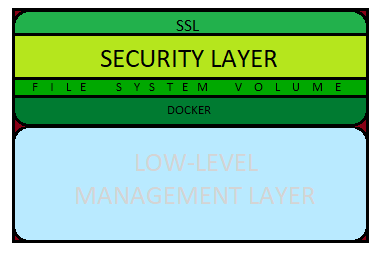
\includegraphics[width=0.6\textwidth]{figures/layer2.png}
    \caption{Módulo de Gestión: Capa de Seguridad}
    \label{layer2}
\end{figure}

Debemos distinguir dos niveles de seguridad en el proceso de ``Ejecución Mixta'':

\begin{itemize}
    \item [--] En primer lugar, hay que garantizar la fiabilidad e integridad de los mensajes intercambiados con la herramienta. Al ser tanto HTTP como WebSockets dos protocolos en los que la información viaja en claro, como texto plano, por el canal de comunicación, decidimos incluir una capa que garantiza seguridad a través del protocolo SSL, que también asegurará que los mensajes no se corrompan. Este nivel tiene un grado bajo de criticidad.
    \item [--] Por otro lado, existe un alto riesgo cuando se trata de permitir que un código cuya fuente es externa se ejecute en nuestro sistema. Esto es precisamente lo que se pretende hacer con esta herramienta, de manera que se debe asegurar que, sea cual sea la fuente del código y su contenido, los problemas de seguridad se pueden contener, evitando que actúen sobre el sistema del cliente, el cual lleva a cabo la ejecución. Esta es una de las funciones del contenedor Docker.
\end{itemize}

Para mantener segura la conexión entre cliente y servidor de ``Ejecución Mixta'' y entre cliente y servidor web a través de Internet utilizamos el protocolo TLS a Nivel de Transporte según la clasificación OSI, que asigna una serie de certificados SSL basados en criptografía asimétrica a cada agente de la comunicación para ser autenticados a la hora de intercambiarse la clave simétrica con la cual se pueden decodificar los datos intercambiados, que viajan encriptados en todo momento. Así funcionan la mayoría de sitios web en la actualidad.

El mayor peso en cuanto a seguridad recae sobre la tarea para la que ha sido diseñada la herramienta. El código que proviene del servidor web puede no ser de confianza o de dudosas intenciones, por lo que no se puede permitir a la ligera su ejecución en la máquina del cliente, dado que esto podría conllevar graves riesgos de pérdida de datos (mediante instrucciones de borrado de disco que viajasen en el código), malfuncionamientos y ataques de toda clase. Por ello, se ha montado lo que se denomina ``volumen'' (Fig. \ref{volumen}) sobre el sistema de ficheros local del servidor de ``Ejecución Mixta'' (cliente web), y se ha restringido el acceso del contenedor Docker y de las instrucciones que en él se ejecutan a este volumen, impidiendo en todo caso que cualquier suceso tenga consecuencias o repercusiones fuera de él. 

\begin{figure}[!hbtp]  \centering\noindent
    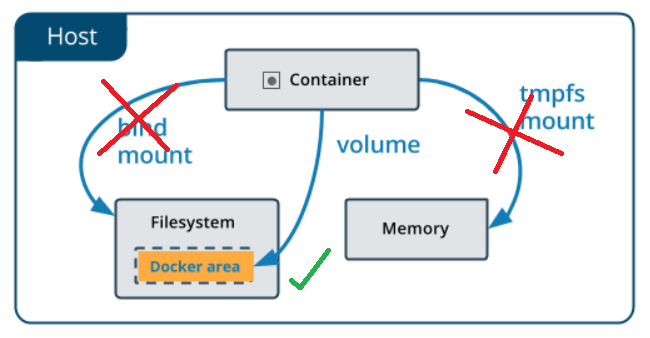
\includegraphics[width=0.75\textwidth]{figures/volumen.png}
    \caption{Volumen de Docker}
    \label{volumen}
\end{figure}

Se puede ver un volumen como una forma de almacenar datos persistentes en el sistema de ficheros local del cliente, necesario para gestionar el acceso al \textit{hardware} entre otras cosas para esta herramienta, que permanece completamente aislado de la funcionalidad central y el \textit{core} de la máquina anfitriona. Esto significa que el contenedor sólo podrá actuar sobre el contenido del volumen y no sobre el contenido externo, pero se podrá beneficiar de todas las ventajas que ofrece el administrador del sistema de archivos del sistema operativo del usuario. Así, aún en el supuesto de que se tratase de utilizar la ``Ejecución Mixta'' en conjunto con una aplicación robótica maliciosa (supuesto muy improbable), el mayor daño posible que se podría causar se reduciría a parar y reiniciar el contenedor, eliminándose todo indicio de código maligno o sospechoso.

\subsubsection{Capa de Bajo Nivel}

La capa de menor nivel y mayor grado de restricción de la herramienta es la que hemos denominado Capa de Bajo Nivel, cuya puerta es sólo visible para el secuenciador del módulo de gestión.
\clearpage
\begin{figure}[!hbtp]  \centering\noindent
    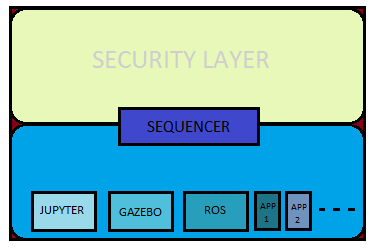
\includegraphics[width=0.6\textwidth]{figures/layer1.png}
    \caption{Módulo de Gestión: Capa de Gestión del Bajo Nivel}
    \label{layer1}
\end{figure}

Una vez resuelta la comunicación y superada la seguridad, el motor de la ``Ejecución Mixta'' debe decidir qué se necesita en todo momento según las peticiones que recibe, y más importante, a quién redirige cada mensaje. Para la Capa de Comunicación, todos los mensajes tienen el mismo destinatario, en función de la conexión HTTPS que se abre para comunicar el lado servidor y el cliente. Este receptor único es un módulo secuenciador, configurado y levantado a través de un \textit{entrypoint} que activará en cada momento la aplicación, herramienta o plataforma auxiliar que se necesite para satisfacer las peticiones de la aplicación robótica, y organizará el canal de bajo nivel para que no se produzcan colisiones durante el proceso. La forma de gestionar la secuenciación se basa en la apertura de nuevos sub-canales de comunicación, ya en un entorno puramente local o \textit{localhost}, y en una redirección de la información obtenida en cada sub-canal hacia el canal HTTPS principal, formateando cada paquete de información según su fuente, su destinatario en la aplicación robótica y su prioridad, a través de cabeceras y estructuras de datos JSON fácilmente procesables por una aplicación web, y accesibles a través del API público de la Capa de Aplicación (Figs. \ref{nb_put_req} y \ref{exec_req}).

\begin{lstlisting}[language=bash, caption=Ejemplo de la parte HTTP de los mensajes]
PUT /api/contents/descarga_bundle.png HTTP/1.1
Host: 127.0.0.1:8888
Connection: keep-alive
Content-Length: 25899
Sec-Fetch-Mode: cors
Origin: http://localhost:8000
User-Agent: Mozilla/5.0 (X11; Linux x86_64) AppleWebKit/537.36
(KHTML, like Gecko) Chrome/77.0.3865.120 Safari/537.36
Content-Type: application/json
Accept: */*
Sec-Fetch-Site: cross-site
Referer: http://localhost:8000/local
Accept-Encoding: gzip, deflate, br
Accept-Language: es-ES,es;q=0.9
\end{lstlisting}

\begin{figure}[!hbtp]  \centering\noindent
    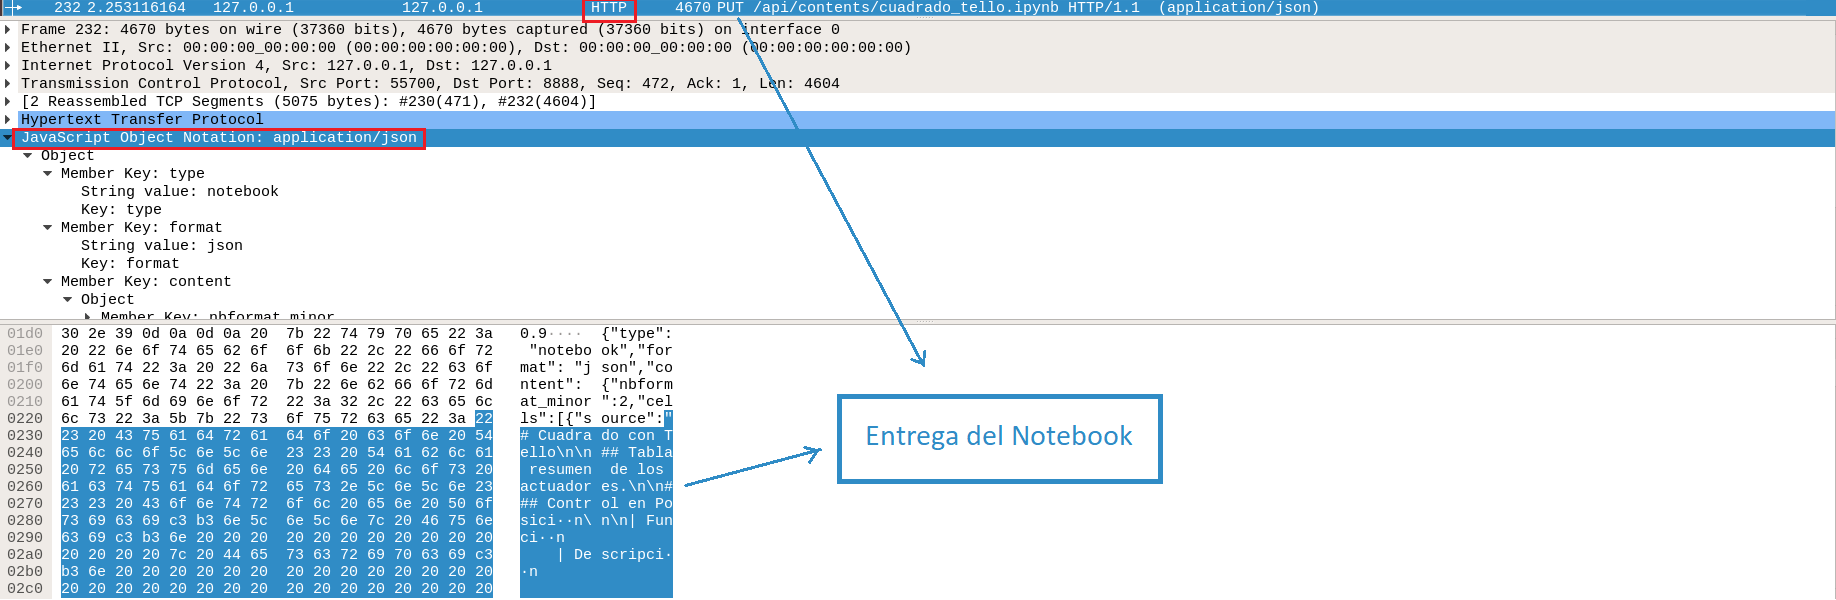
\includegraphics[width=1.05\textwidth]{figures/notebook_put_request.png}
    \caption{Mensaje de Entrega del Cuadernillo o Notebook}
    \label{nb_put_req}
\end{figure}

\begin{figure}[!hbtp]  \centering\noindent
    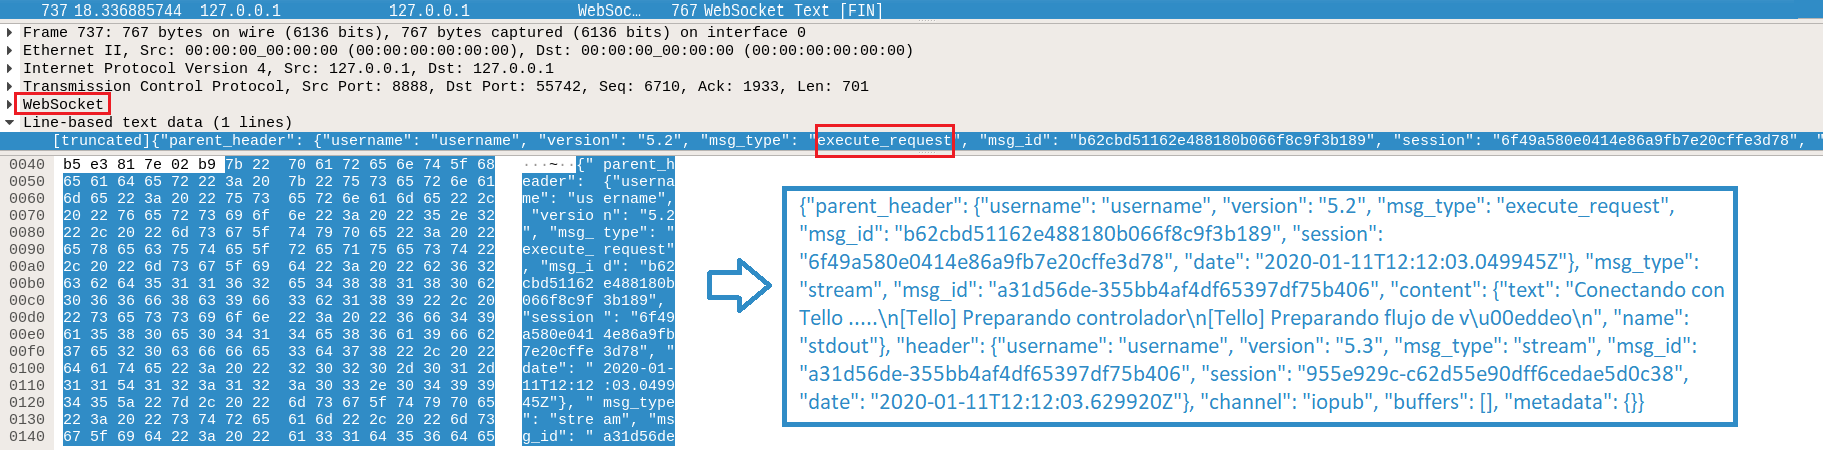
\includegraphics[width=1.05\textwidth]{figures/execute_request.png}
    \caption{Mensaje de Respuesta de Petición de Ejecución }
    \label{exec_req}
\end{figure}

Además, los diferentes programas que ejecutan en el interior del contenedor Docker en el servidor de ``Ejecución mixta'' necesitan un mecanismo de intercomunicación de tipo p2p, sin pasar por todo el mecanismo de transmisión, recepción y procesado descrito anteriormente como parte de la arquitectura, para facilitar la colaboración entre ellos sin sucumbir a problemas de tipo \textit{jitter}, grandes retardos de extremo a extremo o pérdidas de información y largas esperas de reenvios que caracterizan a muchos enlaces de Internet basados en TCP/IP. Para implementar este mecanismo de comunicación interna aprovecharemos las herramientas de ROS, donde el secuenciador tendrá el rol de \textit{MASTER} y las diferentes plataformas y aplicaciones en ejecución actuarán como suscriptores y publicadores de información a través de \textit{topics} conocidos por todos. Así, se dispondrá por ejemplo un HAL API (\textit{Hardware Abstraction Layer}) que permitirá a todos los programas que lo requieran el acceso a las interfaces de sensado y actuación del robot, ya sea real (con \textit{plugins} y \textit{drivers} reales involucrados) o simulado (con \textit{drivers} virtuales). Este método de intercomunicación facilita el crecimiento de la red de agentes (que simplemente ``escuchan'' la información del canal que les conviene y publican los datos que generan que pueden resultar útiles para otros procesos) que se puede lanzar para proporcionar mayor volumen de información a la aplicación robótica remota, y por tanto a la construcción de aplicaciones remotas más ricas que no produzcan carga computacional en el lado servidor de la misma gracias a la ``Ejecución Mixta''.

\section{Funcionamiento}
\subsection{Flujograma}

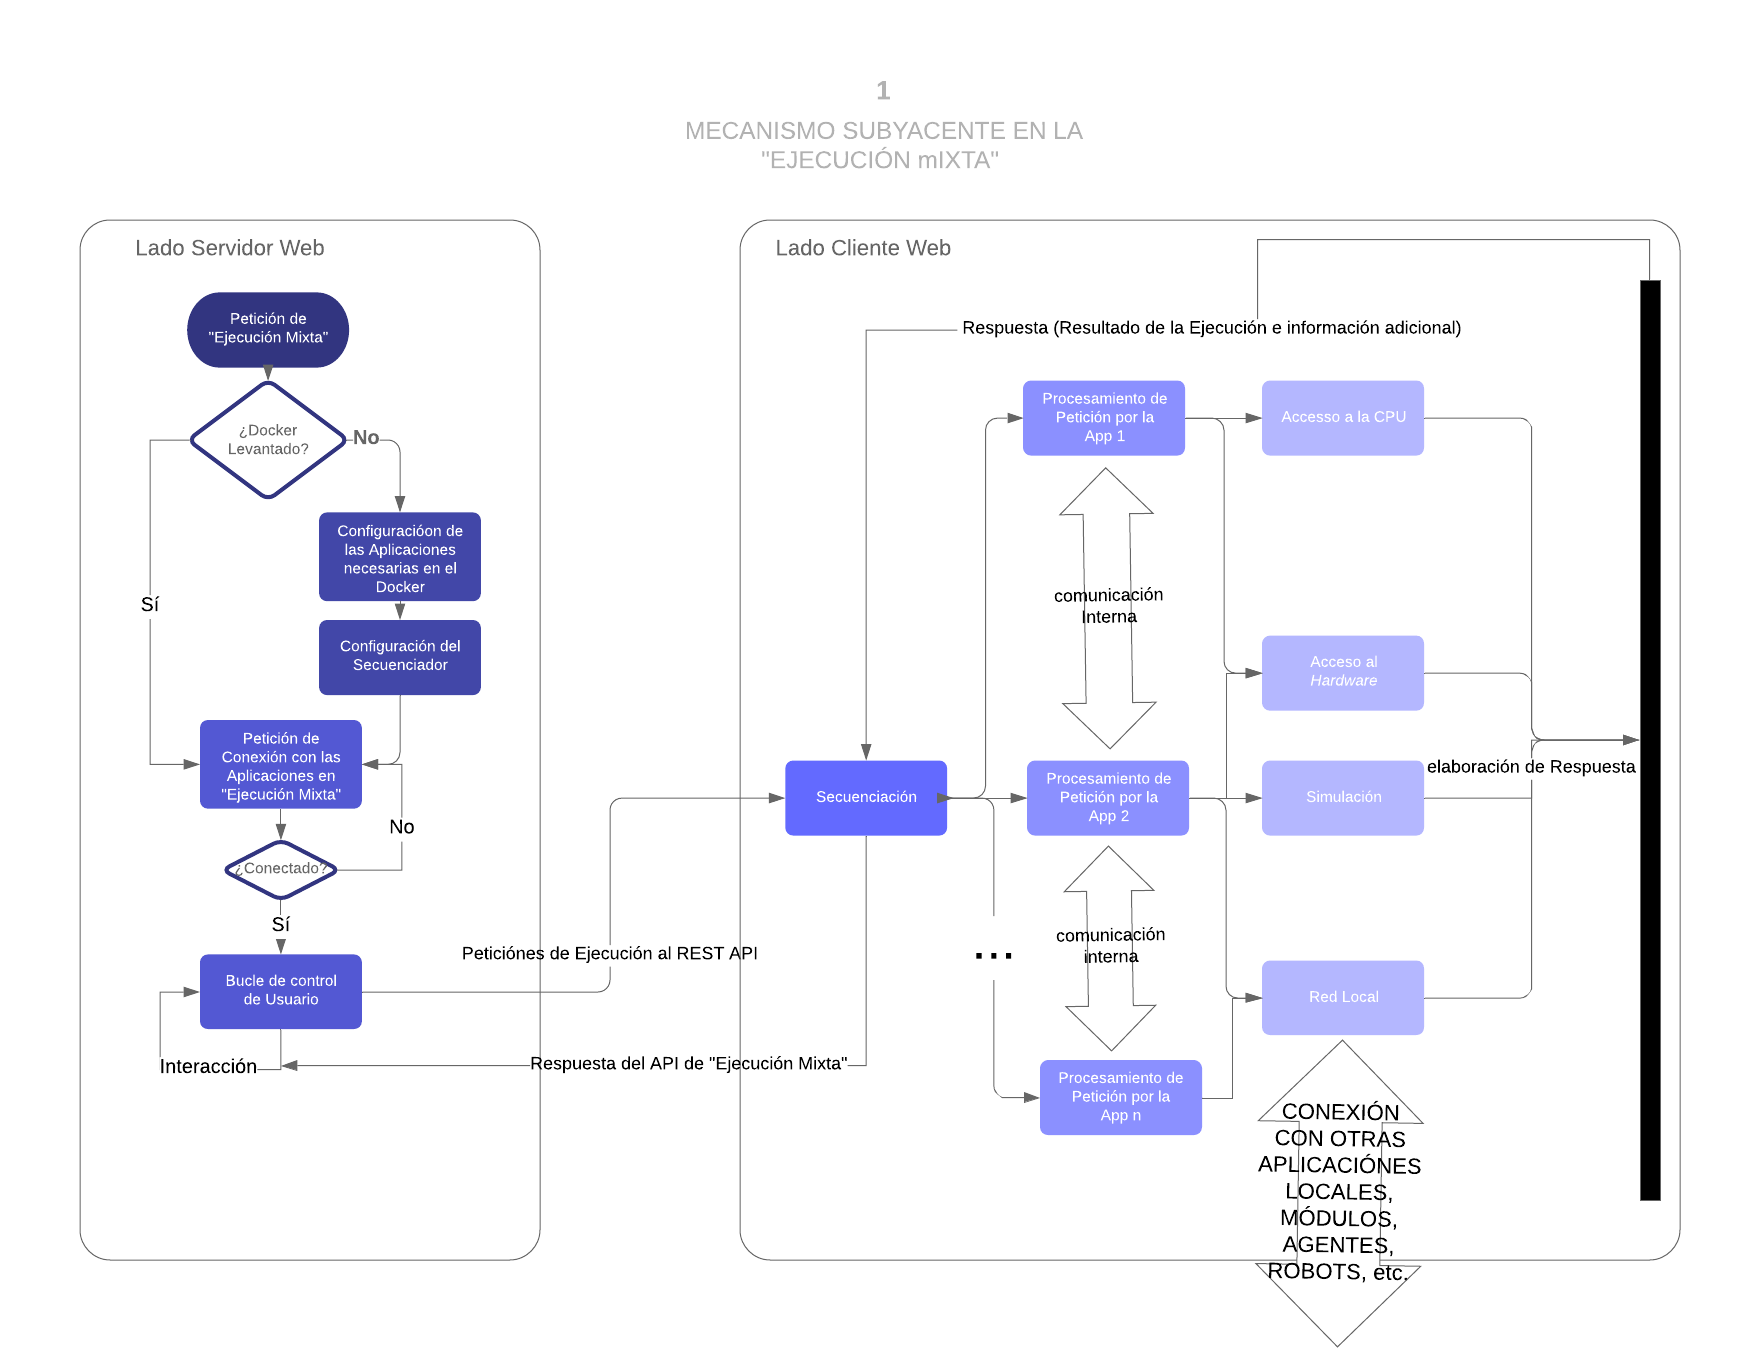
\includepdf[addtolist={1,figure,{Flujograma},flowchart}]{figures/flowchart.png}

\subsection{Ejecución Mixta: Diagrama de flujo}

Para explicar el mecanismo que desata el uso de la ``Ejecución Mixta'' por parte de una aplicación, se utilizará el caso hipotético de un usuario que dispone de un robot móvil con conectividad inalámbrica a través de una red propia con visibilidad a la red local del usuario, al ser la del robot una subred de ésta.

Apoyándonos en el diagrama de flujo anterior (Fig. \ref{flowchart}), el proceso comienza con la realización de la petición inicial de ``Ejecución Mixta'', que se corresponde con la solicitud hecha por el usuario a la aplicación remota de un servicio que utiliza senda herramienta de ejecución. Dado que la aplicación web remota es la que ofrece el servicio solicitado, es también la aplicación la que conoce la configuración de ``Ejecución Mixta'' necesaria para el proceso, así como la combinación de aplicaciones de las que va a requerir información durante la ejecución que deben iniciarse en el lado cliente web. Es entonces cuando se envía esta configuración al cliente, quien debe iniciar el contenedor Docker que aloja la herramienta. Una vez iniciado, se ha de conectar con cada una de las aplicaciones contenidas en la herramienta de ejecución desde la aplicación web. Como se mencionó con anterioridad, esto desencadena en el servidor web una petición inicial al API de ``Ejecución Mixta'', que pasa a desempeñar el rol de cliente de ``Ejecución Mixta'', y que hace una solicitud de conexión. Si los mecanismos de seguridad se resuelven con éxito, el secuenciador del lado cliente web, que actúa como servidor de ``Ejecución Mixta'', garantiza el acceso de la aplicación remota a la ejecución. Es entonces cuando se inicia el servicio que el cliente web solicitó en primera instancia, ingresando en un bucle de control y eventos de la misma forma que sucedería en cualquier otro tipo de aplicación web. En este bucle, la aplicación web atiende permanentemente las interacciones del usuario web, quien generará eventos en el contexto de la aplicación web, y que podrá generar peticiones concretas de ejecución local. Cuando se produce este tipo de petición es cuando la aplicación hace uso de la ``Ejecución Mixta'' para lanzar el código del usuario web, escrito y almacenado remotamente desde su punto de vista, sobre el \textit{hardware} local al usuario. Como se comentó, estas peticiones viajan con un formato concreto a modo de protocolo con destino al secuenciador de ``Ejecución Mixta'', quien ya en el entorno local es capaz de analizar la petición y redirigirla convenientemente a su destinatario o destinatarios. Los receptores finales de estas solicitudes serán las diferentes aplicaciones lanzadas para soportar el servicio web, que se especificaban en el \textit{entrypoint} de configuración inicial del secuenciador. Es entonces cuando los receptores pueden procesar la petición, siempre y cuando el método solicitado esté soportado por el REST API de ``Ejecución Mixta''. El receptor principal será siempre Jupyter, pues es quién tendrá la capacidad de ejecutar código sobre la CPU local o el robot. También habrá un volumen considerable de peticiones de simulación, con el fin de mantener siempre actualizado el estado de la simulación, si existe, en la aplicación web y su interfaz gráfico, que es el que ve el usuario. Para el caso planteado, incluso habrá peticiones concretas o resultados de la ejecución del código que desembocarán en el establecimiento de un nuevo canal de comunicación a través de la red del cliente web. Como se puede ver en el diagrama anterior, este canal se puede utilizar para conectar el resultado de la ``Ejecución Mixta'' a cualquier otra aplicación externa del lado servidor de ejecución preparada para recibir los mensajes de respuesta que se generan. Esto hace crecer la potencia y el alcance de la ejecución, y las posibilidades de servicio web que se puede ofrecer. En el caso del ejemplo, la ejecución generaría mensajes que deben ser enviados al receptor del robot móvil a través de la red inalámbrica, que se materializarían en la actualización de sus actuadores y sensores. Según sea el mensaje, el robot devolverá cierta información. Con esta información, y la proveniente del resultado del procesamiento de la petición entrante por cada aplicación receptora, se compone un único mensaje de respuesta que se reenvía a través del API al servidor web, con toda la información que el servicio espera para su correcto funcionamiento. El ejemplo para este caso pueden ser mensajes de éxito o fracaso de acceso a las interfaces del robot y el resultado concreto de la ejecución solicitada. La información se usa en última instancia para actualizar el interfaz y el estado del servicio para que el cliente web pueda ver el resultado de su interacción. Se finalizaría así la iteración del proceso de ``Ejecución Mixta'' y quedaría a la espera de nuevas peticiones hasta la solicitud de finalización de ejecución, con la cual se liberaría la memoria asignada a todos los procesos en el lado servidor de ejecución y se detendría el contenedor de forma segura, pudiéndose dar por terminado el servicio web.
	\chapter{Implementación de la ``Ejecución Mixta''}
En este capítulo se explica cómo se implementó la idea planteada paso a paso, detallando minuciosamente cómo se alcanzó cada uno de los hitos mencionados y aportando la explicación técnica de los problemas encontrados y las soluciones propuestas.

\section{Proceso de Implementación}

Del mismo modo que no se puede comenzar la casa por el tejado, no podemos empezar con la implementación del mecanismo de la ``Ejecución Mixta'' sin una aplicación robótica a la que conectarla. Por tanto, el primer paso del proceso de construcción fue desarrollar el primer contenido que se quería servir a través de la ``Ejecución Mixta''. Para ilustrar el funcionamiento y la orientación de la herramienta que queríamos crear, decidimos organizar el contenido a servir como una aplicación para el aprendizaje de distintos ámbitos de la robótica por medio de ejercicios con contenido académico. Dado el origen de la idea, resulta lógico que la temática del primer ejercicio tuviese que ver con la visión artificial. En la prueba de concepto que supone este primer prototipo no se quiso poner mucho énfasis en la calidad o utilidad del mismo, sino simplemente comenzar por obtener una primera versión completamente funcional para crecer a partir de ella, como se explicó en la sección de metodología. Por tanto, se comenzó por desarrollar a través de Jupyter un \textit{Notebook} que debía actuar como interfaz de edición de la aplicación (IDE), el cual a su vez iba a ser el encargado de formar muchos de los mensajes y protocolos de ejecución del código del usuario en un entorno local. El comienzo por este contexto puramente local supone el asumir que el código servido por la aplicación robótica proviene de la misma máquina, en la misma red. Este primer cuadernillo se usaría posteriormente para desarrollar el resto de módulos y con fines depurativos. El cuadernillo define un ejercicio consistente en un sencillo filtro de color, una de las tareas más simples de la visión artificial que suele aparecer en todo proyecto de esta rama de la robótica. El objetivo del mismo es hacer el \textit{tracking} de un objeto de la imagen en base a cierta propiedad, en este caso su color, para obtener su posición en cada fotograma proporcionado por la fuente de vídeo. Se desarrolló por tanto un \textit{backend} de ejercicio basado en un bucle de iteraciones con intervalo variable (en función de la duración de ejecución de un ciclo) que actúa como ``plantilla'' que permite al usuario colocar su código y que éste se comporte de manera cíclica, con una serie de métodos a su disposición para facilitar el proceso de desarrollo de su código como parar, restablecer o ejecutar la lógica. El primer reto a resolver es el acceso a la fuente de imágenes, también como parte de esta infraestructura del ejercicio. Sea cual sea la naturaleza del servidor de vídeo (un fichero estático almacenado en el sistema de archivos, un dispositivo de vídeo integrado o un sensor de vídeo conectado al equipo a través de USB) es necesario solventar el acceso al \textit{hardware} del cliente web. Para el caso concreto de los sensores de imagen existe mucha funcionalidad resuelta que ya permite acceder a los dispositivos de vídeo detectados en el sistema anfitrión, que se puede obtener a través de \textit{plugins} de ROS o incluso haciendo uso de funciones empaquetadas en OpenCV. Cabe mencionar que éstos métodos solucionan el acceso nativo, pero aún hay que montar sobre él un mecanismo que permita introducir la información del sensor en el contenedor Docker, desde donde quedará accesible para el \textit{kernel} de Jupyter y, por tanto, utilizable y procesable por el usuario desde el editor de código dado, pero esto se explicará más adelante. Se optó por ambas herramientas para implementar una fuente de vídeo configurable y así abrir la posibilidad de seleccionarla de entre las opciones antes propuestas. Una vez conectado el código al flujo de vídeo, se continuó con la infraestructura de soporte del filtro de color que incluye funcionalidad gráfica de visualización mediante el envío de las imágenes crudas y procesadas por canales WebSockets, módulos de control de flujo para controlar la ejecución iterativa del código y poder implementar algoritmos reactivos y métodos con funcionalidad específica resuelta para poder trabajar en la solución al ejercicio que se ofrecen a través de un API de ejercicio al usuario. Todo ello se ubica en la ``Ejecución Mixta'' como una aplicación auxiliar que se ejecutaría como un agente de la capa de Bajo Nivel dentro del contenedor, y que aportaría la opacidad que se perseguía de cara a que el usuario no lidiase con problemas asociados al \textit{hardware} y al bajo nivel, sino que dispusiese de las imágenes de su fuente a través de una sencilla instrucción en su código, y pudiese trabajar con ellas y visualizarlas con la misma facilidad. Para terminar con la construcción del primer ejercicio, se implementó una solución de referencia al mismo con una posible vía para obtener el resultado esperado, principalmente haciendo uso de las librerías OpenCV para el tratamiento digital. Aunque los algoritmos planteados para los ejercicios no son objeto de esta tésis, se describe brevemente a continuación el funcionamiento del filtro propuesto:
\clearpage
\begin{center}
Ante la imagen de entrada
\end{center}
\begin{figure}[!hbtp]  \centering\noindent
    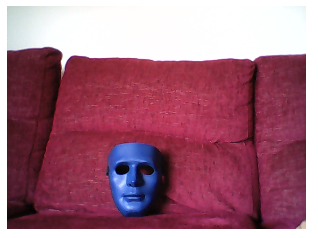
\includegraphics[width=0.65\textwidth]{figures/cf_input.png}
    \caption{Input: Fotograma de la Fuente de Vídeo}
    \label{input}
\end{figure}

Se aplicaría, en primer lugar, un suavizado a la imagen de entrada con un filtro Gaussiano para eliminar o reducir el posible ruido y, con él, los falsos positivos en el filtro. Luego convertiríamos el espacio de color de la imagen de entrada, típicamente RGB o BGR, al espacio HSV, donde resulta mucho más sencillo establecer límites para el filtrado de determinado color dado que esta característica se encuentra completamente representada en la componente H, además de ser un espacio mucho más robusto a los cambios en intensidad de luz. Por último, se aplican los límites para obtener una imagen umbral binaria en la que los píxeles de la imagen de entrada cuyo valor de la componente H está entre las cotas establecidas quedan reflejados en la imagen B/N como píxeles de primer plano (de valor 255), y el resto de píxeles se etiquetan como píxeles de fondo (de valor 0). Para señalar el objeto que supera el filtro, bastaría con hacer una aproximación rectangular a los contornos del objeto blanco de la imagen umbral (detectados en aquellas regiones en las que la derivada es muy grande, cambios rápidos de píxeles blancos a negros). Se escoge el contorno más grande localizado para asegurar la identificación de todo el conjunto de píxeles que forman el objeto. Se pueden aplicar otras técnicas para mejorar el filtrado y eliminar ruido, como operaciones morfológicas o técnicas de post-procesado.
\begin{figure}
\centering
\begin{subfigure}{.32\textwidth}
  \centering
  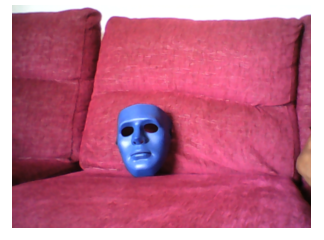
\includegraphics[width=.95\linewidth]{figures/cf_smooth.png}
  \caption{Suavizado de la Imagen}
  \label{smooth}
\end{subfigure}
\begin{subfigure}{.32\textwidth}
  \centering
  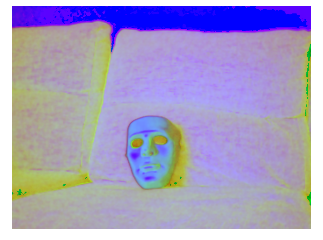
\includegraphics[width=.95\linewidth]{figures/cf_hsv.png}
  \caption{Conversión a HSV}
  \label{hsv}
\end{subfigure}
\begin{subfigure}{.32\textwidth}
  \centering
  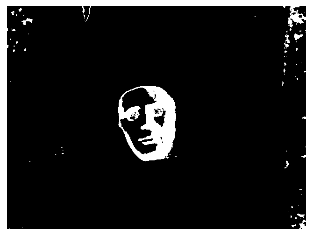
\includegraphics[width=.95\linewidth]{figures/cf_mask.png}
  \caption{Imagen Umbralizada}
  \label{mask}
\end{subfigure}
\caption{Procesado de Imagen para el Filtro de Color}
\label{procesado}
\end{figure}

El proceso descrito se muestra gráficamente en la Fig. \ref{procesado}. De esta manera, nuestro cuadernillo de Jupyter tendría ya la lógica que resuelve el filtro, además de un recubrimiento de código auxiliar que contendría el \textit{back-end} del ejercicio con los métodos de acceso a la fuente de vídeo, de recogida de imágenes, de visualización y control, etc. En la interfaz de Jupyter se pueden mostrar en todo momento las imágenes que reflejan el estado del proceso a través del API de programación de ejercicio y varias librerías gráficas (entre ellas OpenCV y matplotlib), como se ve en la Fig. \ref{ui_cf_jupyter}.

\begin{figure}[!hbtp]  \centering\noindent
    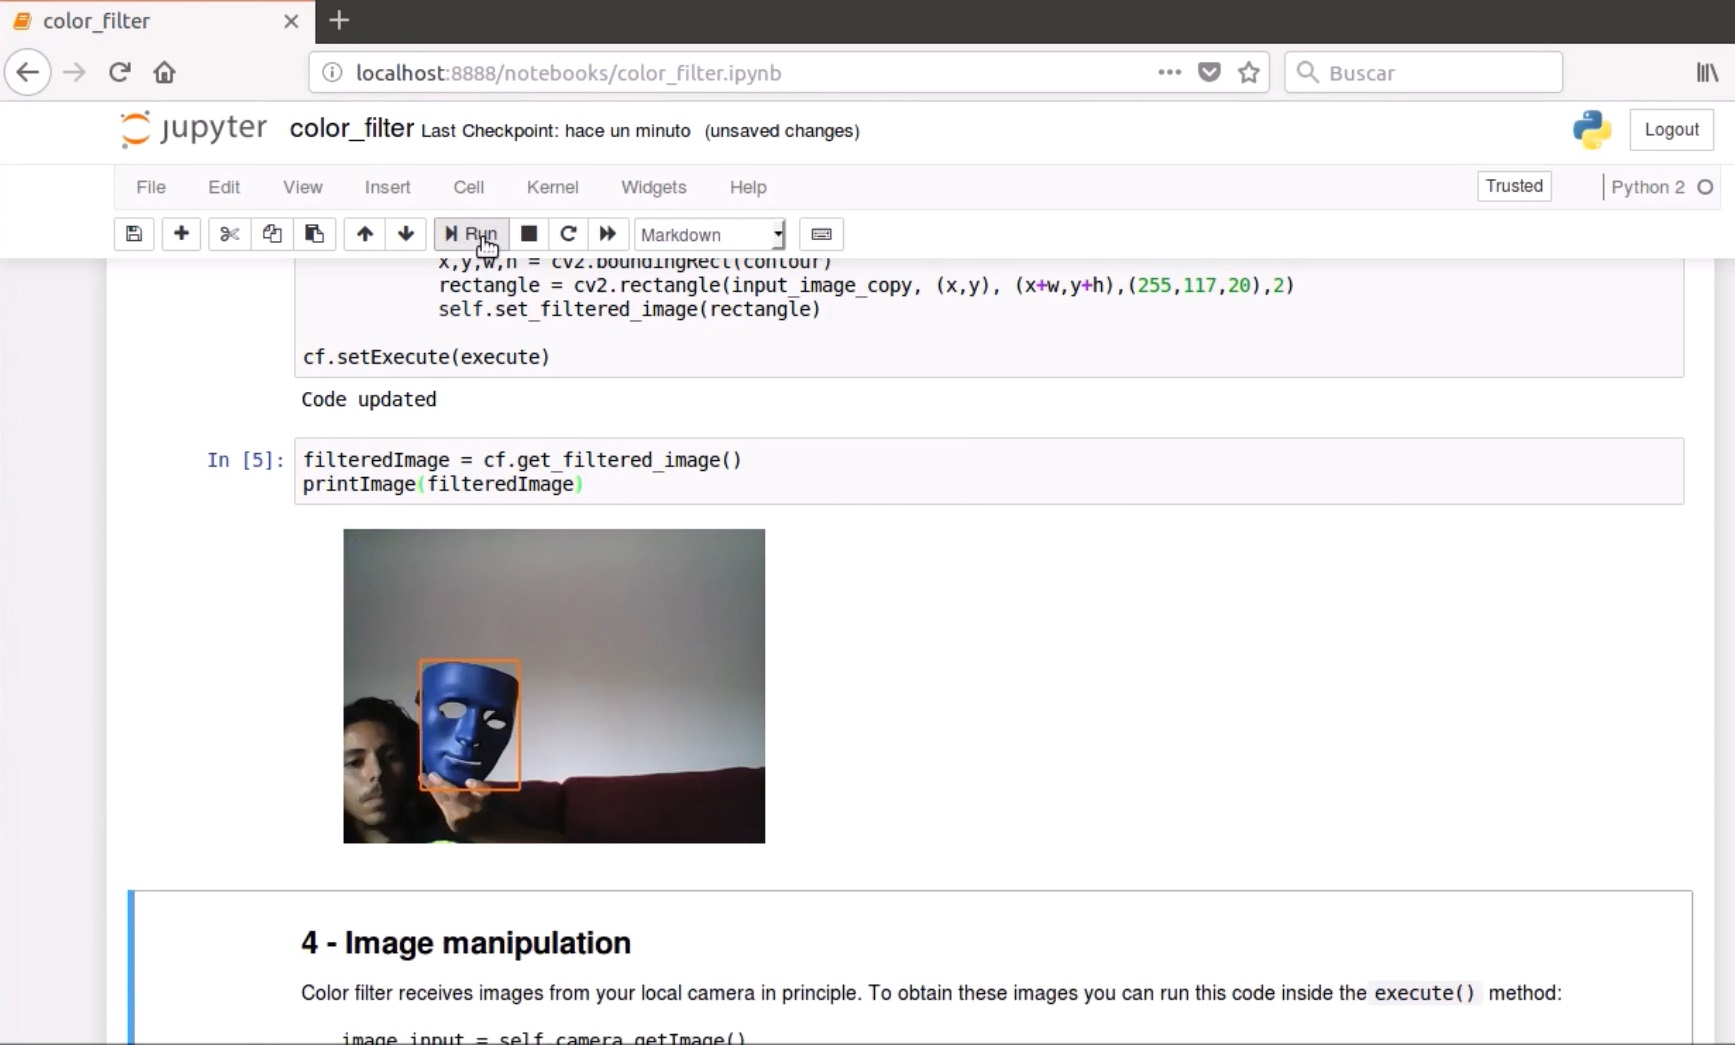
\includegraphics[width=0.99\textwidth]{figures/ui_cf_jupyter.jpg}
    \caption{UI de Jupyter para el Filtro de Color}
    \label{ui_cf_jupyter}
\end{figure}

En este punto, disponemos de una versión completamente local del prototipo de herramienta que queremos construir. Por tanto, y tras la investigación correspondiente, se procedió a la implementación de un \textit{local runtime}, es decir, de un entorno de ejecución utilizando un \textit{kernel} local. Había que desarrollar un servidor remoto que contuviese la aplicación y el modelo de ejercicio creado y que, ante una nueva petición del ejercicio, estableciese una comunicación fluida con el \textit{kernel} del cliente para coordinar la ejecución en su \textit{hardware}, por medio del lanzamiento del servidor de ``Ejecución Mixta'' en su máquina. 

Se construyó un pequeño servidor muy básico a través de Django (Fig. \ref{appui}) con capacidad para atender a un cliente que solicitase un ejercicio por medio de un click en el interfaz web, y se colocó en una máquina externa. Debajo del botón sobre el que se hace click, sucedería todo el mecanismo de enlazado y comunicación para disponer el entorno mixto.

\begin{figure}[!hbtp]  \centering\noindent
    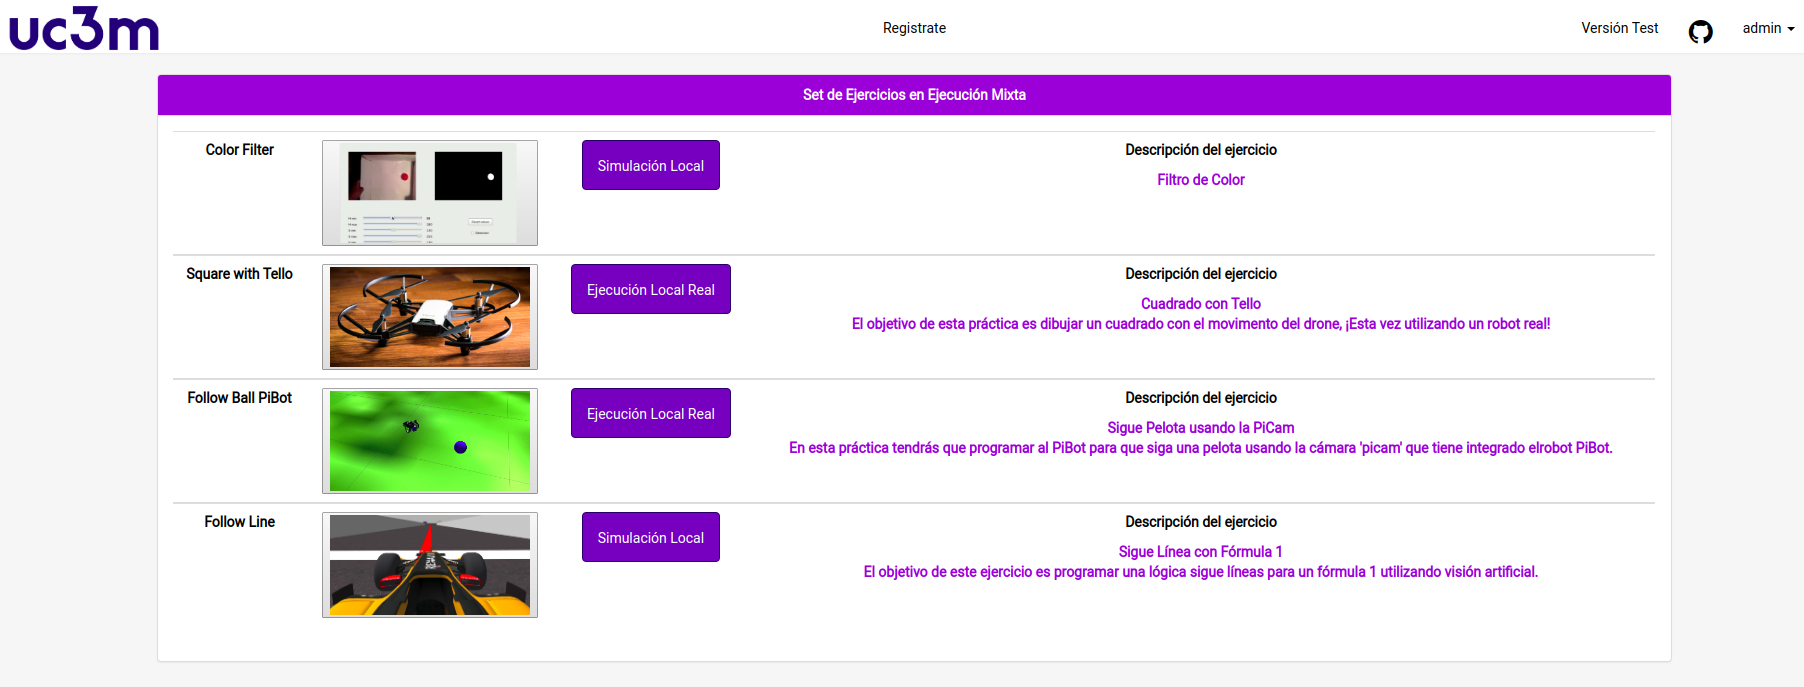
\includegraphics[width=0.99\textwidth]{figures/app_ui.png}
    \caption{UI de la Aplicación en Django}
    \label{appui}
\end{figure}

\begin{figure}[!hbtp]  \centering\noindent
    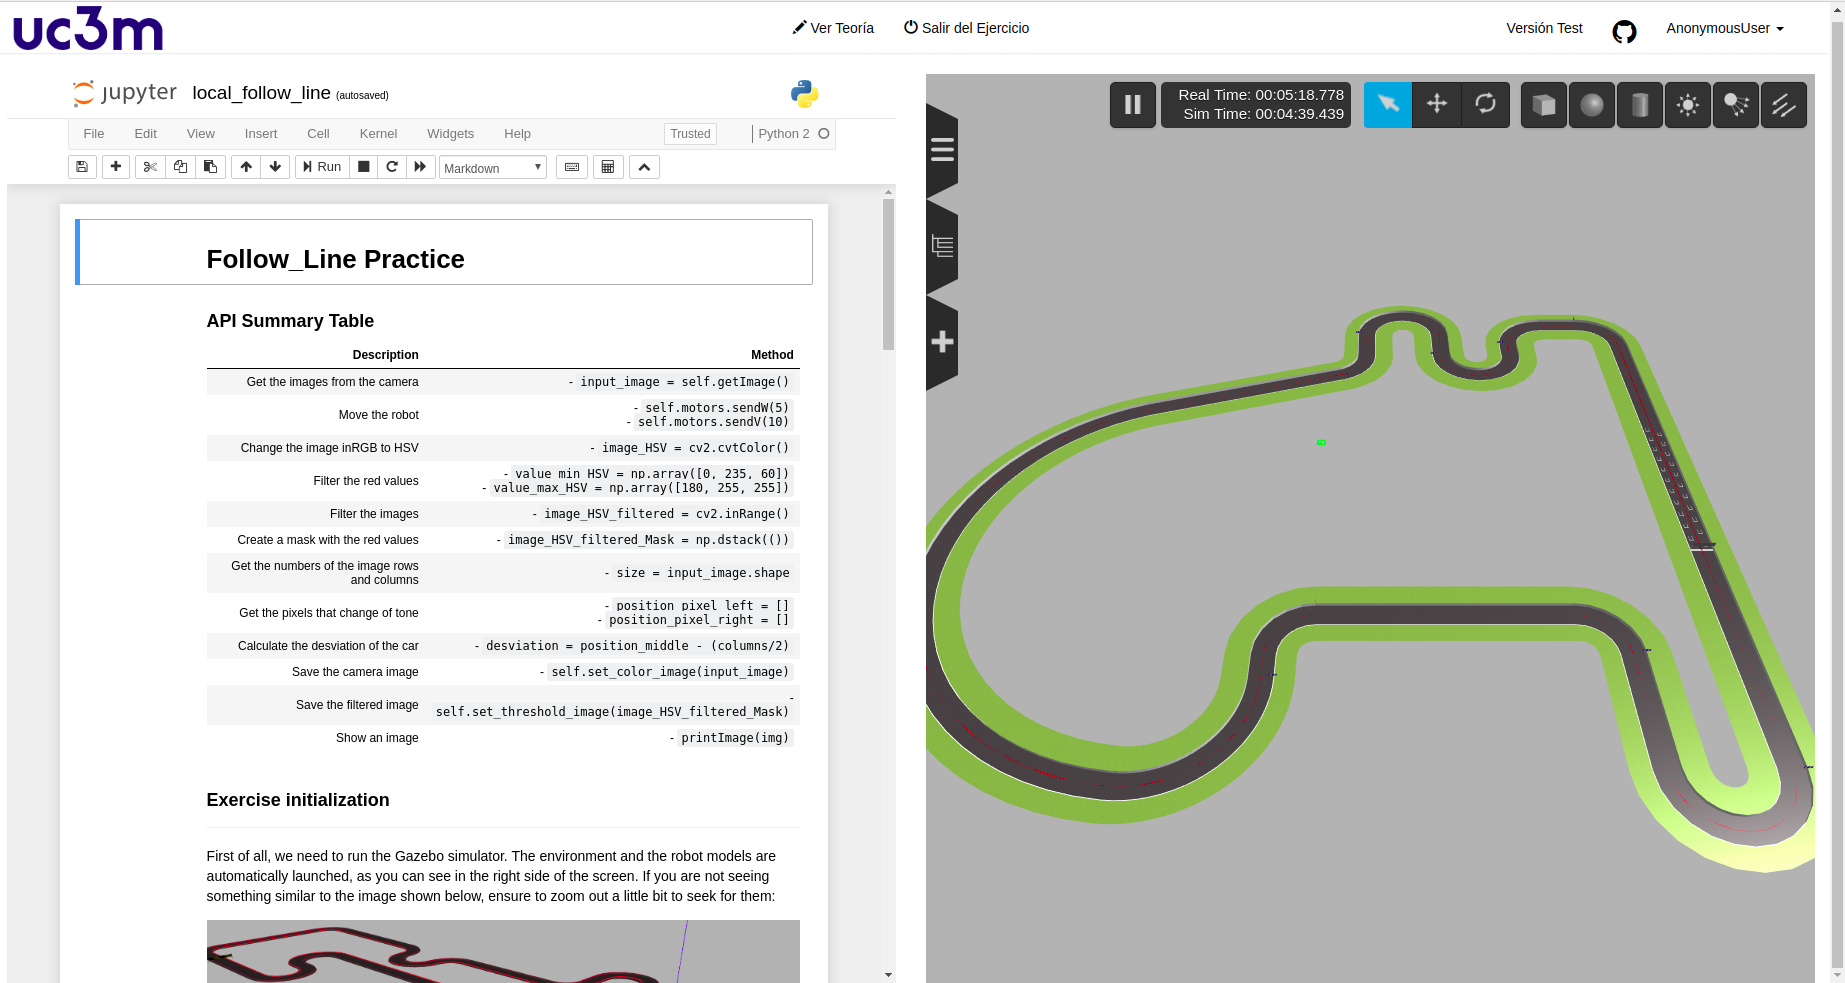
\includegraphics[width=0.99\textwidth]{figures/ui_simulation.png}
    \caption{UI de Simulación de la Aplicación}
    \label{simui}
\end{figure}

Como se puede ver en la imágenes (Fig. \ref{simui}) de la interfaz que ofrece el servidor web a su cliente, es necesario para el correcto funcionamiento de la herramienta que el receptor principal de los mensajes de ``Ejecución Mixta'' sea Jupyter, y por tanto también tiene sentido que se use como editor de código. Tras la conexión HTTPS con el servidor web, el cliente especifica su dirección IP y el puerto en que está corriendo el servidor de Jupyter en su máquina, de tal manera que se puede establecer fácilmente un puente que permita que el servidor acceda a los datos generados por Jupyter en un punto remoto, y los ofrezca al usuario como parte del interfaz, a través del mecanismo de paso de mensajes de actualización periódicos. Esto requiere hacer unos cambios sobre el servidor provisto por el proyecto Jupyter con el fin de abrir el acceso a él desde el exterior, no sin antes establecer los correspondientes métodos de seguridad. Se profundizó en la arquitectura de servicio de Jupyter para poder adaptar su funcionamiento a nuestras necesidades. Luego, como paso previo a la visualización y ejecución del código del cliente localmente a través de órdenes generadas en el interfaz ofrecido por un servidor remoto, se hace indispensable proveer al servidor de ``Ejecución Mixta'', concretamente al \textit{kernel} de Jupyter, del código asociado al ejercicio para que pueda ejecutarlo. Aquí comienza el mecanismo de establecimiento y supervisión de la conexión HTTPS de la Capa de Comunicación. La conexión con Jupyter puede hacerse de manera sencilla mediante el envío de un simple mensaje bajo el método OPTIONS, al que el servidor responderá con toda la información que necesitamos para el establecimiento de la conexión a través de cabeceras HTTP, entre ellas el \textit{token} de autenticación de Jupyter, los métodos y tipos de contenido que se aceptan, y el código CSRF\footnote{\href{https://www.geeksforgeeks.org/what-is-cross-site-request-forgery-csrf/}{What is CSRF and how to prevent it?}} necesario para enviar información al servidor.

Estudiamos el mecanismo de comunicación de la plataforma, que emplea principalmente el protocolo ZeroMQ\footnote{\url{https://zeromq.org/}} o 0MQ para el intercambio asíncrono de mensajes \textit{N-a-N} a través de la web. Esto nos proporciona, además de una plantilla para los tipos de mensajes que debemos enviar al \textit{kernel} de Jupyter, una idea bastante fiel del proceso que desencadena cada órden o petición que se le hace al servidor de Jupyter. También se utilizó \textit{sniffers}\footnote{\href{https://www.wireshark.org/\#1398253364-1-69}{Wireshark Sniffer}} para monitorizar el funcionamiento local de Jupyter (Fig. \ref{wireshark}). Este paso fue vital para comprender el procedimiento que debíamos seguir para iniciar una sesión de Jupyter completa y válida.

\begin{figure}[!hbtp]  \centering\noindent
    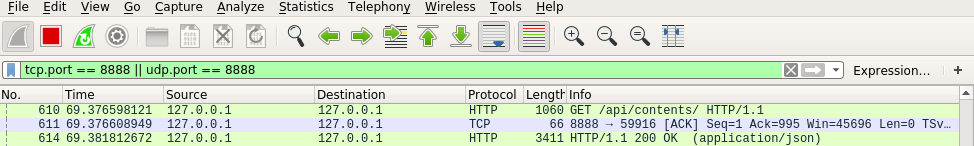
\includegraphics[width=0.99\textwidth]{figures/wireshark.png}
    \caption{Capura de Paquetes del Mecanismo de Comunicación de Jupyter}
    \label{wireshark}
\end{figure}

Tras el establecimiento, se puede comenzar con el intercambio de mensajes 0MQ. Aprovecharemos el REST API que ofrece Jupyter para la comunicación con el \textit{kernel} en tanto que este \textit{RESTfull Service}\footnote{\href{https://docs.oracle.com/javaee/6/tutorial/doc/gijqy.html}{What is a RESTfull Service?}} ofrece todo lo necesario para enviarle ficheros de código, órdenes de ejecución, órdenes de control (reinicio, apagado, encendido, pausa, cambio de lenguaje, limpieza de salidas, etc.) (Fig. \ref{jupyter_rest_api}) y, en general, lo necesario para facilitar el uso de la plataforma a través de la web. Por tanto, por el canal de ``Ejecución Mixta'' estaríamos enviando, principalmente, mensajes HTTP sobre una capa de TLS con datos de tipo 0MQ en el cuerpo, destinados a Jupyter.

\begin{figure}[!hbtp]  \centering\noindent
    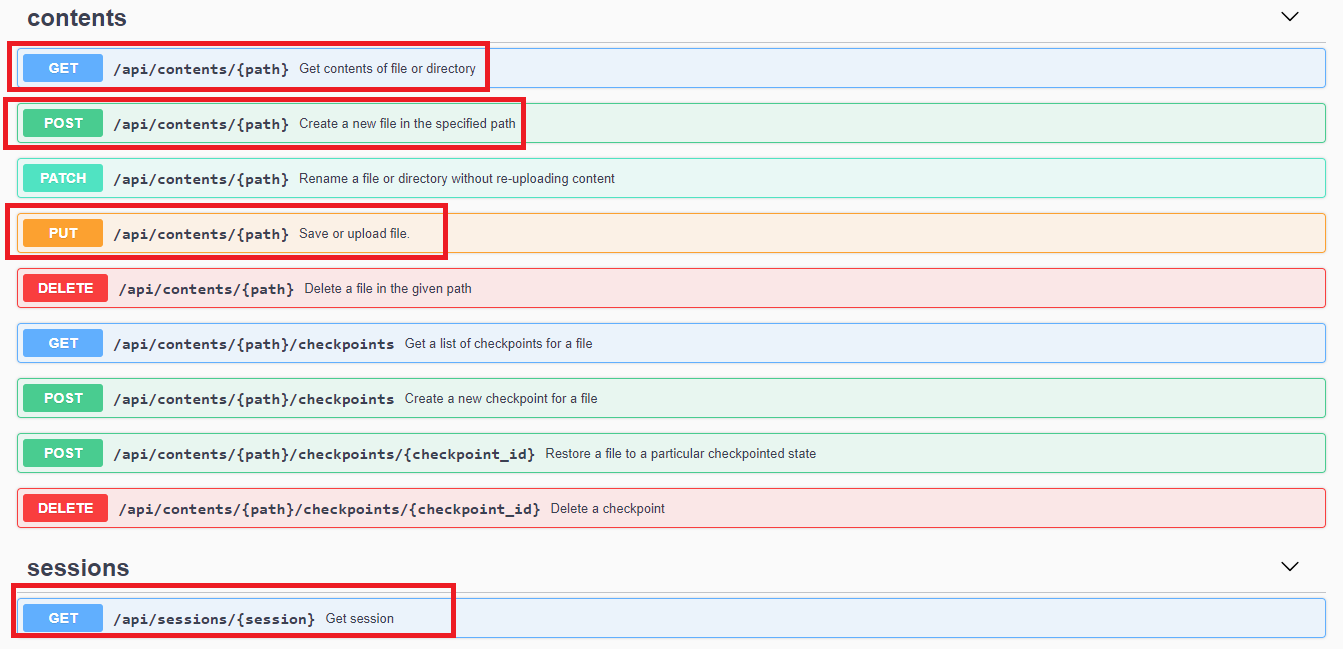
\includegraphics[width=0.99\textwidth]{figures/jupyter_rest_api.png}
    \caption{REST API de Jupyter}
    \label{jupyter_rest_api}
\end{figure}

En base al conocimiento obtenido del motor de comunicación de Jupyter, seleccionamos aquellos métodos del REST API que necesitaríamos, marcados en la imagen superior. Se muestra a continuación un ejemplo del mensaje que se enviaría al servidor de Jupyter para hacer llegar el código al \textit{kernel} encargado de un cuadernillo concreto:

\lstset{
   language=JavaScript,
   backgroundcolor=\color{lightgray},
   extendedchars=true,
   basicstyle=\footnotesize\ttfamily,
   showstringspaces=false,
   showspaces=false,
   numbers=left,
   numberstyle=\footnotesize,
   numbersep=9pt,
   tabsize=2,
   breaklines=true,
   showtabs=false,
   captionpos=b
}
\begin{minipage}{\linewidth}
\begin{lstlisting}[caption=Formato de Mensajes de ``Ejecución Mixta'']
const url = 'http://'+_ip+':'+_port+'/api/contents/' + nbname;
const data_put = ' {"type": "notebook",
                    "format": "json",
                    "content": ' + nbcontent + '} ';
const message = {
        headers:{'Content-Type':'application/json',
                 //'Authorization': 'token ' + _token,
                },
        body:data_put,
        method:"PUT"
};
\end{lstlisting}
\end{minipage}

donde cada variable que aparece en el mensaje (\textit{\_ip, \_port, nbname,\_token, nbcontent}) sería establecida por el servidor web y contendría la dirección del servidor Jupyter y el contenido y nombre del cuadernillo que queremos enviar. El formato de todos los mensajes es similar, en tanto que se trata de peticiones HTTP como se puede ver en la constante \textit{message} con el formato de cuerpo 0MQ que se refleja en la constante \textit{data\_put}. Este tipo de mensajes, con su respectiva codificación, constituye el tipo de mensajes a intercambiar por la herramienta ``Ejecución Mixta'' para el establecimiento y envío iniciales.

El proceso de comunicación con Jupyter comenzaría por el establecimiento de la conexión, donde se crea una sesión de ejecución, continuaría con el envío del código del cuadernillo y de cada fichero de código de aplicación auxiliar que necesite el ejercicio, para acabar con una orden de inicio del \textit{kernel} del lenguaje adecuado encargado de la ejecución, que se montará sobre un núcleo latente en el sistema del cliente web. La utilización de direcciones IP públicas, el protocolo HTTP (estándar de Internet) que utiliza por defecto el puerto 8080 (puerto de Internet, abierto a mensajes transportados sobre TCP o UDP por la red, con cualquier origen) que puede atravesar \textit{firewalls} y resolver conexiones sea cual sea el dominio público, y el \textit{token} de autorización embebido en los mensajes garantizan la conectividad y la integridad de la sesión de Jupyter, así cómo el funcionamiento entre sistemas bajo distintas redes o sub-redes de la misma red.

En este punto del desarrollo, hemos superado el principal obstáculo de la ``Ejecución Mixta'' e implementado un mecanismo capaz de ejecutar código entre redes, con actualización de los resultados en tiempo real en ambos lados servidor  y cliente web. Se completa así el primer ciclo de trabajo, no sin antes realizar los tests convenientes de funcionamiento y desempeño y el análisis de los resultados. La herramienta ya es capaz de conectar un código remoto (aplicación robótica) con un ``robot'' local (cámara). Se propusieron los siguientes pasos y analizaron los riesgos, donde salió a la luz la necesidad de utilizar contenedores Docker (lo cual cambiará sustancialmente el mecanismo de comunicación) y la posibilidad de enriquecer la aplicación robótica con otros procesos dentro de él, para dar soporte de simulación y ampliar el \textit{hardware} utilizable.

Hubo que estudiar el motor de Docker y su funcionamiento para crear un \textit{DockerFile} con instrucciones en lenguaje SHELL para virtualizar una distribución Ubuntu con todas las herramientas y aplicaciones auxiliares involucradas en la ``Ejecución Mixta'', para que utilizar la herramienta resultase tan fácil como descargar la imagen Docker y levantar el contenedor. Utilizar un contenedor Docker para empaquetar los procesos necesarios e incluir seguridad supone añadir complejidad el mecanismo de comunicación, en tanto que Docker levanta su propia sub-red dentro de la red del cliente, lo que nos deja una intratable sub-red dentro de una red distinta desde el punto de vista del servidor web. Se replanteó el mecanismo de comunicación para que utilizase el navegador del cliente web como intermediario entre el usuario y la aplicación robótica, el cual sí que tiene conectividad directa con una sub-red de su propia red. Por tanto, el servidor web abre ahora una comunicación con el \textit{browser} del cliente en lugar de directamente con el servidor Jupyter, y éste actúa como \textit{proxy} reenviando cada mensaje donde corresponde a través de una secuenciación programada en código JavaScript, de manera que tanto de cara al cliente como al servidor web, la comunicación sigue siendo la misma que en el paso anterior, esta vez con un origen o destinatario distinto. Simplemente se trata de añadir la lógica del \textit{proxy} para que viaje con la aplicación que se sirve al usuario web. El navegador ya utiliza protocolos como STUN o ICE que permiten descubrir e interaccionar con ambas partes del mecanismo. Así, los mensajes reenviados por el navegador serán recibidos por el módulo secuenciador de ``Ejecución Mixta'', que procesará la información que llega para orquestar el correcto inicio del entorno y los agentes, traduciendo las órdenes JavaScript iniciales a comandos de lanzamiento (Listing. 5.2) y entregando las órdenes de ejecución a quien corresponda (Listing. 5.3). Ahora se tiene un prototipo completo y seguro, capaz de funcionar sobre Docker y a través de Internet, con ambos extremos situados en cualquier punto.

\begin{lstlisting}[language=bash, caption=Código de Inicio del Secuenciador]
#!/bin/bash

rm -rf /tmp/.X0-lock

Xvfb -shmem -screen 0 1280x1024x24 &

source /opt/jderobot/setup.bash
source /opt/ros/kinetic/setup.bash
source /opt/jderobot/share/jderobot/gazebo/gazebo-assets-setup.sh
export PYTHONPATH=$PYTHONPATH:/home/jderobot/.exercises

cd ~/gzweb
npm start &

cd ~/volume/user/exercise

jupyter nbextension enable hide_input/main --user
jupyter nbextension enable init_cell/main --user
jupyter notebook --ip=0.0.0.0 --allow-root &

cd ~

EXTENSION=`echo "$1" | cut -d'.' -f2`
if [ $EXTENSION = "world" ]
  then
    roscore &
fi

if ! [ -z "$2" ]
  then
    python ~/referees/$2 &
fi

if ! [ -z "$1" ]
  then
    EXTENSION=`echo "$1" | cut -d'.' -f2`
    if [ $EXTENSION = "launch" ]
      then
        roslaunch /opt/jderobot/share/jderobot/gazebo/launch/$1
    else
        rosrun gazebo_ros gazebo /opt/jderobot/share/jderobot/gazebo/worlds/$1
    fi
else
    tail -f /dev/null
fi
\end{lstlisting}
\begin{lstlisting}[language=bash, caption=Reenvío de Mensajes]
[I 11:51:09.187 NotebookApp] Saving file at /thumbnail_follow_line.png
[Gazebo] Sat Jan 11 2020 11:51:09 GMT+0000 (Coordinated Universal Time) Received Message: {"op":"advertise","id":"advertise:~/heartbeat:14","type":"heartbeat","topic":"~/heartbeat"} from http://127.0.0.1:8080 ::ffff:172.17.0.1
[Python Process] Sat Jan 11 2020 11:51:09 GMT+0000 (Coordinated Universal Time) Received Message: {"op":"publish","id":"publish:~/heartbeat:15","topic":"~/heartbeat","msg":{"alive":1}} from http://127.0.0.1:8080 ::ffff:172.17.0.1
[I 11:51:11.758 NotebookApp] 302 GET /notebooks/world.png (172.17.0.1) 0.95ms
[I 11:51:11.847 NotebookApp] Adapting to protocol v5.1 for kernel 368a1e46-acc2-4976-acf3-25528ae77d77
\end{lstlisting}

El API de inicio de la ``Ejecución Mixta'' fue enriquecido con la aparición de los parámetros característicos de Docker que permiten crear un puente seguro entre un elemento virtualizado y su homólogo en la máquina anfitrión. Un ejemplo de esto es el mecanismo que ya anticipábamos para el acceso a la cámara integrada en el sistema cliente desde el interior de un contenedor Docker, resuelto con el mapeo \textit{-v /dev/video0:/dev/video0}, o la redirección de interfaces de escucha del sistema a sus correspondientes dentro del contenedor (\textit{-p 8888:8888 -p 8889:8889 -p 8080:8080}).

Llegados a este punto, se trata de enriquecer la ``Ejecución Mixta'' para que además de ejecutar lógica pueda simular y usar aplicaciones auxiliares como \textit{plugins} o \textit{drivers} robóticos. Utilizamos ROS dada su fácil integración con Gazebo y el lenguaje Python, que nos permite construir una aplicación completa y autocontenida asociada al código del ejercicio que, lanzada en el interior del contenedor de ``Ejecución Mixta'', creará el mecanismo de inter-comunicación a través de mensajes de ROS que orquestará el funcionamiento de un código que se ejecuta en una aplicación para que sus resultados se reflejen en la simulación y en la aplicación web al mismo tiempo. Lo mismo sucederá con robots reales sustituyendo el simulador por un controlador del dispositivo \textit{hardware}, empleando el mismo mecanismo interno de mensajes (Listings. 5.4 y 5.5). Cada mensaje que deba viajar hacia la aplicación con información relevante será recogido a través de un canal WebSockets por el secuenciador del módulo de gestión situado en el navegador, envuelto con una capa HTTPS y enviado al servidor remoto para que este lo procese (Fig. \ref{mixedexecarch}).

\begin{lstlisting}[language=bash, caption=Topics de ROS asociados a los Canales de Comunicación Internos]
~$ rostopic list
/F1ROS/cameraL/camera_info
/F1ROS/cameraL/image_raw
/F1ROS/cameraL/parameter_descriptions
/F1ROS/cameraL/parameter_updates
/F1ROS/cmd_vel
/F1ROS/odom
/clock
/gazebo/link_states
/gazebo/model_states
/gazebo/parameter_descriptions
/gazebo/parameter_updates
/gazebo/set_link_state
/gazebo/set_model_state
/rosout
/rosout_agg
/tf
\end{lstlisting}

\begin{minted}[
    gobble=4,
    frame=single,
    linenos
  ]{yaml}
    # follow_line.yml
    Camera:
      Topic: "/F1ROS/cameraL/image_raw" 
      Name: follow_line_camera
    
    
    Motors:
      Topic: "/F1ROS/cmd_vel"
      Name: follow_line_motors
      MaxV: 40
      MaxW: 2
    
    Websockets:
      Host: 0.0.0.0 
      Port: 9002
      SSL: False
      Cert: '/etc/certs/fullchain1.pem' 
      Key: '/etc/certs/privkey1.pem'
\end{minted}
\begin{lstlisting}[caption=Configuración de Canales del Secuenciador en formato YAML]
\end{lstlisting}

Una vez dispuesto el contenedor Docker, completamos otro ciclo y verificamos que la ``Ejecución Mixta'' ya no supone ninguna carga de cómputo para el lado servidor de la aplicación web, y también que podemos eliminar el proceso de instalación, dado que todas las dependencias están agrupadas en el contenedor. Lanzar la ``Ejecución Mixta'' pasa ahora por utilizar el API de Docker de control de contenedores, que pondrá en marcha todos los sub-sistemas necesarios para el funcionamiento de la aplicación robótica y los dejará disponibles para su consulta desde el exterior, por parte del servidor remoto a través del secuenciador o \textit{proxy} web. Así, la aplicación puede enviar cualquier tipo de orden de ejecución en formato Python al servidor de Jupyter, que materializará esa orden en el simulador Gazebo a través de los canales ROS o, incluso, en el robot o sensor real conectado al sistema del cliente. La aplicación robótica le indicará al secuenciador qué sub-procesos necesita para el funcionamiento de un ejercicio robótico concreto.

Para implementar el soporte de simulación, se diseñó un sistema de configuración que permite indicar los elementos, robots y características que debe tener la escena simulada a través de Gazebo (Fig. \ref{gzworld}), haciendo uso de ficheros de extensión \textit{.world} o \textit{.launch}, siendo los primeros un subconjunto del lenguaje de marcado XML que indica los agentes involucrados en la simulación (Listing. 5.7), y el segundo un configurador inteligente que permite lanzar, además del mundo de simulación, una serie de nodos que se puedan necesitar para controlar por ejemplo las interfaces de un determinado robot (Listing. 5.6). 

\begin{lstlisting}[language=XML, caption=Configuración de Lanzamiento de Simulaciones]
<?xml version="1.0" encoding="UTF-8"?>
<launch>
  <!-- We resume the logic in empty_world.launch, changing only the name of the world to be launched -->
  <include file="$(find gazebo_ros)/launch/empty_world.launch">
    <arg name="world_name" value="f1_1_simplecircuit.world"/> <!-- Note: the world_name is with respect to GAZEBO_RESOURCE_PATH environmental variable -->
    <arg name="paused" value="false"/>
    <arg name="use_sim_time" value="true"/>
    <arg name="gui" value="true"/>
    <arg name="headless" value="false"/>
    <arg name="debug" value="false"/>
    <arg name="verbose" default="false"/>
  </include>  
</launch>
\end{lstlisting}

\begin{lstlisting}[language=XML, caption=Configuración de Lanzamiento de Simulaciones]
<?xml version="1.0" ?>
<sdf version="1.5">
  <world name="default">
    <scene>
      <grid>false</grid>
    </scene>
    <!-- A global light source -->
    <include>
      <uri>model://sun</uri>
    </include>
    <include>
	    <uri>model://pista_simple</uri>
	    <pose>0 0 0 0 0 0</pose>
    </include>
    <include>
      <uri>model://f1_renault</uri>
      <pose>53.462 -10.734 0.004 0 0 -1.57</pose>
    </include>
    <scene>
        <sky>
            <clouds>
                <speed>12</speed>
            </clouds>
        </sky>
     </scene>
  </world>
</sdf>
\end{lstlisting}

\begin{figure}[!hbtp]  \centering\noindent
    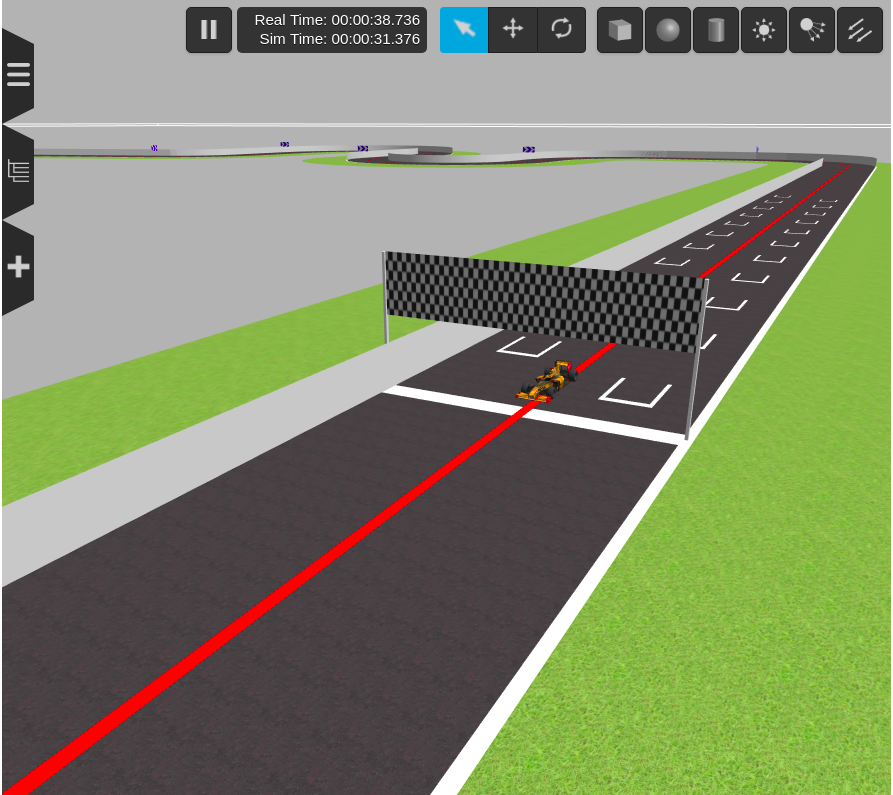
\includegraphics[width=0.9\textwidth]{figures/world_gazebo.png}
    \caption{Escenario de Simulación}
    \label{gzworld}
\end{figure}

Con ello, al lanzar la herramienta se indicará qué fichero de configuración se quiere usar a través de instrucciones del API de ``Ejecución Mixta'', que se ocupará de levantar tanto la simulación como la red de comunicación interna basada en ROS como se puede ver en el \textit{snippet} de código inferior (Listing. 5.8), y la capa de abstracción que permite al usuario programar su robot y acceder a toda la funcionalidad mientras se materializan los cambios en el simulador.

\begin{minted}[
    gobble=4,
    frame=single,
    linenos
  ]{python}
    class ListenerCamera:
        def __init__(self, topic):
            
            self.topic = topic
            self.data = Image()
    
        # [...]
    
        def start (self):
     
            self.sub = rospy.Subscriber(self.topic, ImageROS,
                                        self.__callback)
    
    class PublisherMotors:
     
        def __init__(self, topic, maxV, maxW):
    
            self.maxW = maxW
            self.maxV = maxV
    
            self.topic = topic
            self.data = CMDVel()
            self.pub = rospy.Publisher(self.topic,
                                       Twist,
                                       queue_size=1)
            rospy.init_node("FollowLineF1")
    
        # [...]
    
        def publish (self):
    
            self.lock.acquire()
            tw = cmdvel2Twist(self.data)
            self.lock.release()
            self.pub.publish(tw)
    
    class FollowLine():
        
        def __init__(self):
            cfg = readConfig()
    
            cameraTopic = cfg["Camera"]["Topic"]
            motorsTopic = cfg["Motors"]["Topic"]
            maxv = cfg["Motors"]["MaxV"]
            maxw = cfg["Motors"]["MaxW"]
    
            self.camera = ListenerCamera(cameraTopic)
            self.motors = PublisherMotors(motorsTopic, maxv,
                                          maxw)
    
            # [...]
\end{minted}
\begin{lstlisting}[caption=Creación de la Red Interna de Comunicación]
\end{lstlisting}

Con todo lo anterior ya resuelto, decidimos implementar también el soporte de ejecución compartida haciendo uso de robots reales. Dada la filosofía modular interconectada que se había diseñado hasta este momento, el enfoque para el caso de querer controlar un robot real desde el lado cliente pasaba sencillamente por crear su controlador, e incluirlo como aplicación auxiliar lanzada dentro de la herramienta y orquestada como un módulo más por el secuenciador. Así, se implementó un driver casero para el robot Tello (Listing. 5.9), un cuadricóptero de DJI e Intel cuyo precio de mercado está al alcance del consumidor medio. Una vez hecho el driver en lenguaje Python, se creó un paquete PIP con el objetivo de poder utilizarlo desde el código del usuario, el cual lo importa como una librería normal y corriente y accede a sus funciones y métodos públicos para controlar el dron (Listing. 5.10). 

\begin{minted}[
    gobble=4,
    frame=single,
    linenos
  ]{python}
    #!/usr/bin/env python
    # -*- coding: utf-8 -*-
    
    import socket, threading, time, libh264decoder, cv2
    import numpy as np
    from math import pi as PI
    from speed_thread import SpeedThread
    
    MAX_VEL = 1.5 # m/s
    MIN_VEL = 0.1 # m/s
    MAX_ROT_VEL = 1 # deg/s
    MAX_ROT_VEL = 360 # deg/s
    ORANGE_MIN = np.array([117, 239, 76],np.uint8)
    ORANGE_MAX = np.array([179, 255, 255],np.uint8)
    
    class Tello:
        """Wrapper class to interact with the Tello drone."""
        def __init__(self, local_ip, local_port,
        command_timeout=.2, tello_ip='192.168.10.1',
                     tello_port=8889):
            # vels vector
            #   [
            #       Right(+)/Left(-),
            #       Forward(+)/Backward(-),
            #       Up(+)/Down(-),
            #       Yaw_right(+)/Yaw_left(-)
            #   ]
            self._vels = [0, 0, 0, 0]
            self.abort_flag = False
            self.decoder = libh264decoder.H264Decoder()
            self.command_timeout = command_timeout
            self.response = None  
            self.frame = None  # numpy array BGR
    
            # socket for sending cmd
            # -------------------------------------------
            self.socket = socket.socket(socket.AF_INET,
                                        socket.SOCK_DGRAM)  
            self.tello_address = (tello_ip, tello_port)
            self.socket.bind((local_ip, local_port))
            # -------------------------------------------
    
            # thread for speed control
            # -------------------------------------------
            self.kill_event = threading.Event()
            self.speed_thread = SpeedThread(self)
            # -------------------------------------------
    
            print("Conectando con Tello .....")
            # to receive video -- send cmd: command, streamon
            self.socket.sendto(b'command', self.tello_address)
            print ('[Tello] Preparando controlador')
            self.socket.sendto(b'streamon', self.tello_address)
            print ('[Tello] Preparando flujo de vídeo')
    
            # [...]
\end{minted}
\begin{lstlisting}[caption=Snippet del Driver de Tello]
\end{lstlisting}

\begin{minted}[
    gobble=4,
    frame=single,
    linenos
  ]{python}
    from tello.tello_wrapper import Drone
    tel = Drone('', 9005)
\end{minted}
\begin{lstlisting}[caption=Uso del Driver]
\end{lstlisting}


De manera análoga a lo ya construido, se diseñaron algunos ejercicios más para probar la herramienta bajo distintos pretextos.

\section{Funcionamiento}
\subsection{Flujograma}

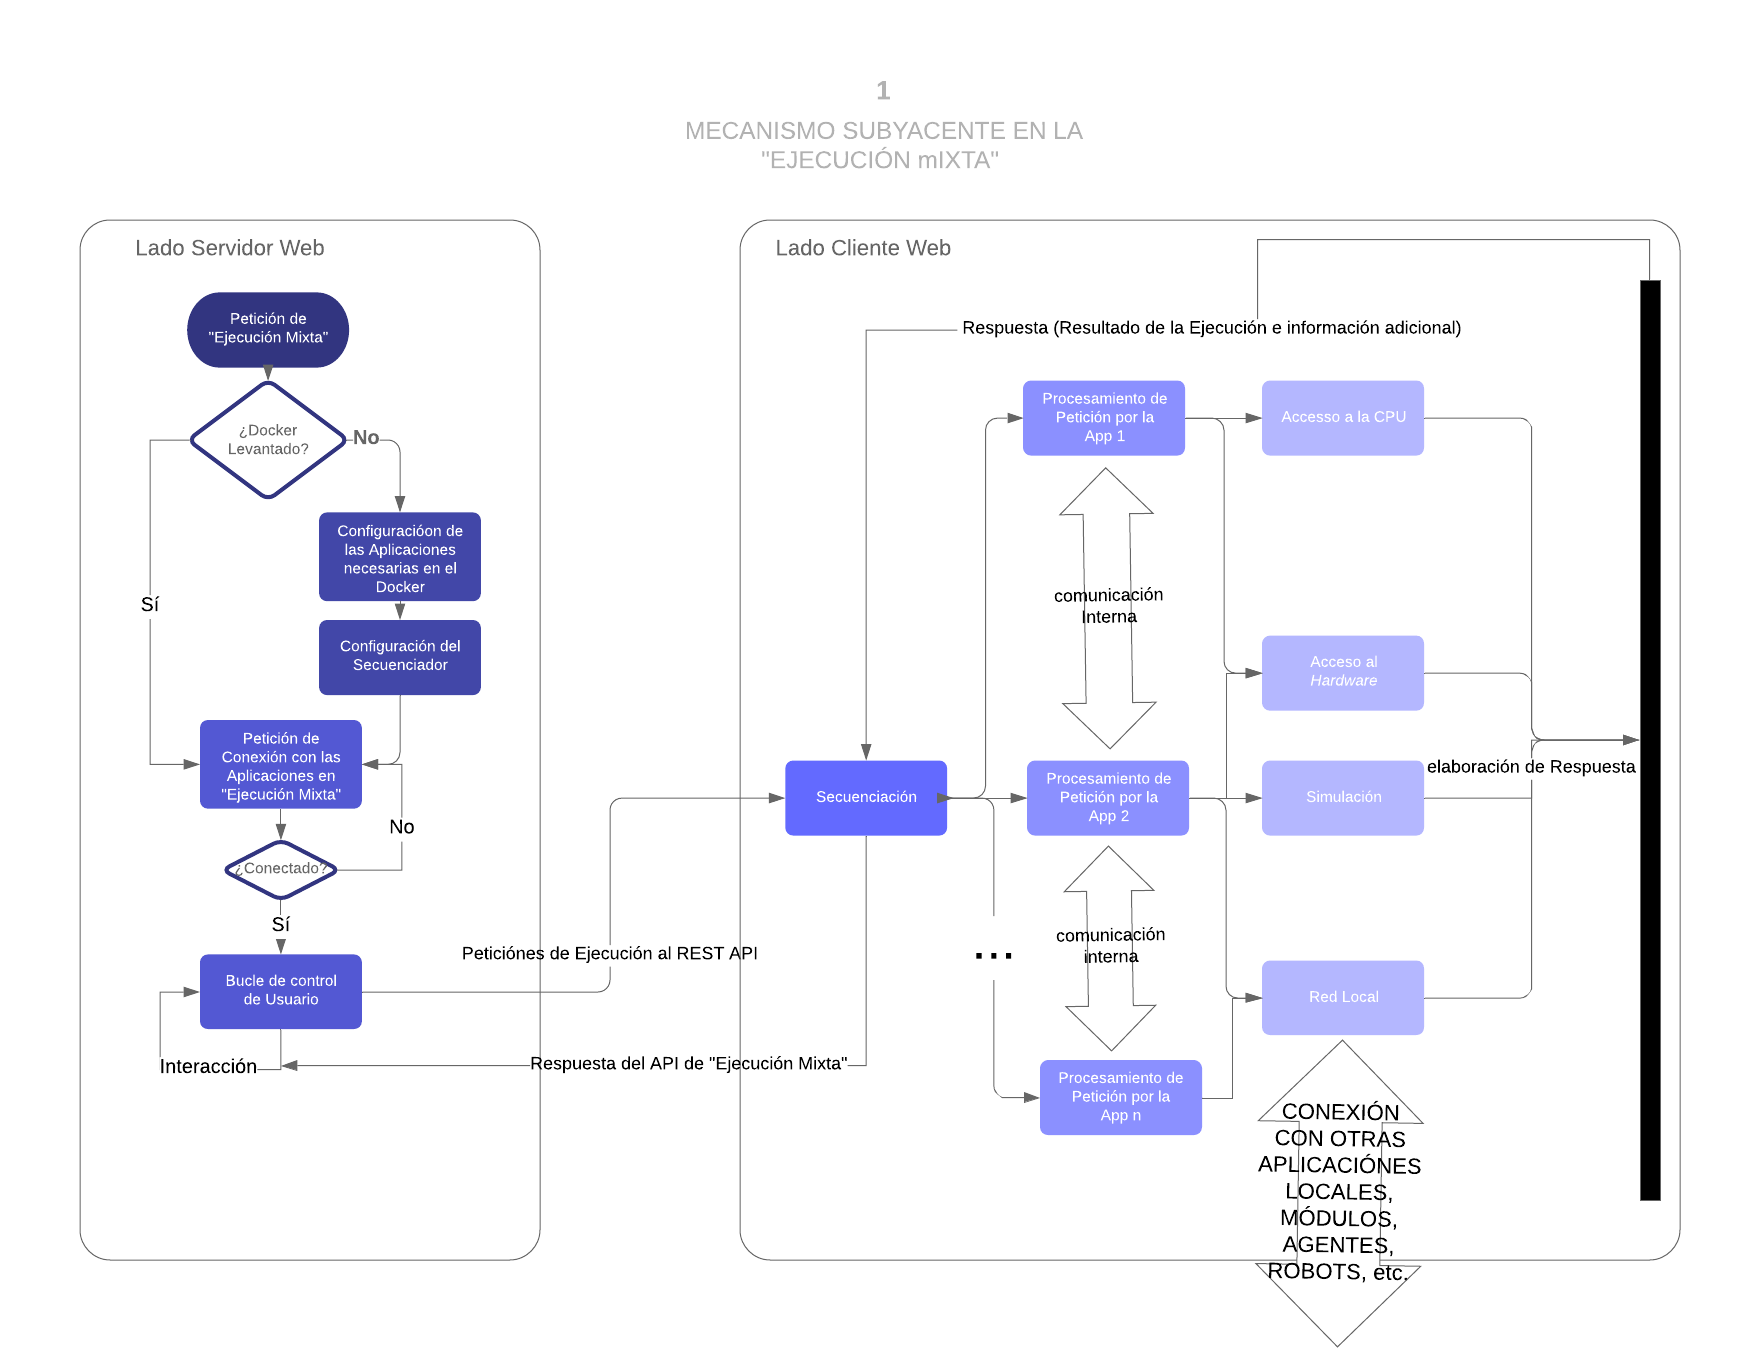
\includepdf[addtolist={1,figure,{Flujograma},flowchart}]{figures/flowchart.png}

\subsection{Mecanismo subyacente de la Herramienta}

Para explicar el mecanismo que desata el uso de la ``Ejecución Mixta'' por parte de una aplicación, se utilizará el caso hipotético de un usuario que dispone de un robot móvil con conectividad inalámbrica a través de una red propia con visibilidad a la red local del usuario, al ser la del robot una subred de ésta.

Apoyándonos en el diagrama de flujo anterior (Fig. \ref{flowchart}), el proceso comienza con la realización de la petición inicial de ``Ejecución Mixta'', que se corresponde con la solicitud hecha por el usuario a la aplicación remota de un servicio que utiliza senda herramienta de ejecución. Dado que la aplicación web remota es la que ofrece el servicio solicitado, es también la aplicación la que conoce la configuración de ``Ejecución Mixta'' necesaria para el proceso, así como la combinación de aplicaciones de las que va a requerir información durante la ejecución que deben iniciarse en el lado cliente web. Es entonces cuando se envía esta configuración al cliente, quien debe iniciar el contenedor Docker que aloja la herramienta. Una vez iniciado, se ha de conectar con cada una de las aplicaciones contenidas en la herramienta de ejecución desde la aplicación web. Como se mencionó con anterioridad, esto desencadena en el servidor web una petición inicial al API de ``Ejecución Mixta'', que pasa a desempeñar el rol de cliente de ``Ejecución Mixta'', y que hace una solicitud de conexión. Si los mecanismos de seguridad se resuelven con éxito, el secuenciador del lado cliente web, que actúa como servidor de ``Ejecución Mixta'', garantiza el acceso de la aplicación remota a la ejecución. Es entonces cuando se inicia el servicio que el cliente web solicitó en primera instancia, ingresando en un bucle de control y eventos de la misma forma que sucedería en cualquier otro tipo de aplicación web. En este bucle, la aplicación web atiende permanentemente las interacciones del usuario web, quien generará eventos en el contexto de la aplicación web, y que podrá generar peticiones concretas de ejecución local. Cuando se produce este tipo de petición es cuando la aplicación hace uso de la ``Ejecución Mixta'' para lanzar el código del usuario web, escrito y almacenado remotamente desde su punto de vista, sobre el \textit{hardware} local al usuario. Como se comentó, estas peticiones viajan con un formato concreto a modo de protocolo con destino al secuenciador de ``Ejecución Mixta'', quien ya en el entorno local es capaz de analizar la petición y redirigirla convenientemente a su destinatario o destinatarios. Los receptores finales de estas solicitudes serán las diferentes aplicaciones lanzadas para soportar el servicio web, que se especificaban en el \textit{entrypoint} de configuración inicial del secuenciador. Es entonces cuando los receptores pueden procesar la petición, siempre y cuando el método solicitado esté soportado por el REST API de ``Ejecución Mixta''. El receptor principal será siempre Jupyter, pues es quién tendrá la capacidad de ejecutar código sobre la CPU local o el robot. También habrá un volumen considerable de peticiones de simulación, con el fin de mantener siempre actualizado el estado de la simulación, si existe, en la aplicación web y su interfaz gráfico, que es el que ve el usuario. Para el caso planteado, incluso habrá peticiones concretas o resultados de la ejecución del código que desembocarán en el establecimiento de un nuevo canal de comunicación a través de la red del cliente web. Como se puede ver en el diagrama anterior, este canal se puede utilizar para conectar el resultado de la ``Ejecución Mixta'' a cualquier otra aplicación externa del lado servidor de ejecución preparada para recibir los mensajes de respuesta que se generan. Esto hace crecer la potencia y el alcance de la ejecución, y las posibilidades de servicio web que se puede ofrecer. En el caso del ejemplo, la ejecución generaría mensajes que deben ser enviados al receptor del robot móvil a través de la red inalámbrica, que se materializarían en la actualización de sus actuadores y sensores. Según sea el mensaje, el robot devolverá cierta información. Con esta información, y la proveniente del resultado del procesamiento de la petición entrante por cada aplicación receptora, se compone un único mensaje de respuesta que se reenvía a través del API al servidor web, con toda la información que el servicio espera para su correcto funcionamiento. El ejemplo para este caso pueden ser mensajes de éxito o fracaso de acceso a las interfaces del robot y el resultado concreto de la ejecución solicitada. La información se usa en última instancia para actualizar el interfaz y el estado del servicio para que el cliente web pueda ver el resultado de su interacción. Se finalizaría así la iteración del proceso de ``Ejecución Mixta'' y quedaría a la espera de nuevas peticiones hasta la solicitud de finalización de ejecución, con la cual se liberaría la memoria asignada a todos los procesos en el lado servidor de ejecución y se detendría el contenedor de forma segura, pudiéndose dar por terminado el servicio web.
    \chapter{Conclusiones y Líneas Futuras}

Este capítulo recogerá las inferencias extraídas durante el desarrollo de esta tesis, mayoritariamente provenientes del periodo de investigación y confirmadas durante la implementación, así como unos ilustrativos casos de uso a modo de conclusión. También dedicará una sección a listar las líneas futuras de investigación que podrían potenciar el desarrollo o abrir nuevos frentes para hacerlo más completo.

\section{Conclusiones} 

Se distinguen dos grupos de conclusiones dada la estructura del presente proyecto que tienen relación con el planteamiento inicial de objetivos y el desarrollo e implementación en sí, respectivamente.
En primer lugar cabe destacar que la herramienta desarrollada cumple los 4 sub-objetivos propuestos en primera instancia, así como todas las características deseables para un fácil y versátil acceso a aplicaciones robóticas. Además, la implementación final cuenta incluso con algunas propiedades no programadas en el planteamiento original, que lo hacen más robusto y seguro.

Se ha llevado a cabo un proceso completo de estudio de herramientas relacionadas con la robótica y su accesibilidad, además de algunas otras con aparente carencia de dicha relación con el campo tecnológico robótico cuyos usos pueden ser replanteados para cumplir alguna función que sí tiene relación. Se ha desarrollado la capacidad de elección y la destreza necesarias para seleccionar un subconjunto de herramientas, aplicaciones y entornos que condujeron a la solución propuesta para un problema sin solución clara previa, además de la habilidad de discernir entre necesidad de desarrollar comportamientos y lógicas desde cero y la posibilidad de adaptar un programa o aplicación existente para que encajara en las necesidades del trabajo. Se consiguió descartar las vías que pudieran suponer no llegar a la solución o un cuello de botella en el desarrollo de la misma, llegando finalmente a la propuesta de un método válido y de funcionamiento verificado por distintas vías que constituye una buena solución para la idea expuesta entre todas las plausibles para este problema no abordado previamente. El cumplimiento de los objetivos demuestra que se ha desarrollado la capacidad de orientación, dirección y ejecución de un proceso de desarrollo asociado a una nueva idea, sin ser necesario el disponer de un guión preestablecido o un esquema de trabajo.
En cuanto al periodo de implementación, se extrajo una serie de conclusiones más específicas acerca de la herramienta desarrollada, la coyuntura tecnológica en relación a la robótica y del modo de trabajar al enfrentarse a un proyecto robótico:
\begin{itemize}
    \item [-] Los primeros pasos de este proyecto desembocaron en un problema sin aparente solución, el cual fue abordable cambiando el enfoque inicial, algo muy común en proyectos tecnológicos. Esto arrojó luz sobre el método de ``trabajo previo’’ que es altamente recomendable llevar a cabo antes de empezar un proyecto: plantear un estudio previo de la viabilidad del mismo y de cada uno de los módulos que se quiere incluir en el diseño. Así pues, se dedujo que no sólo la implementación debe estar sujeta a un proceso iterativo de verificación de calidad como el planteado inicialmente, sino que también  el estudio debe estar sujeto a una constante supervisión en la que se busque mejorar la idea o el método e incluso en la que se replanteen los objetivos por el bien final del proyecto, lo que permite lidiar con potenciales imprevistos e incrementar la robustez y calidad.
    \item [-] Comprender el funcionamiento latente de los agentes que se utiliza en un desarrollo facilita mucho su integración y permite aprovechar la flexibilidad que pueden ofrecer. Así pues, a la hora de escoger entre distintas opciones se ha de ser estricto y restrictivo con los objetivos que se pretende alcanzar, dado que suele haber diferentes soluciones a un mismo problema. Personalmente considero que el software robótico es muy versátil hoy en día gracias a las arquitecturas distribuidas y modulares que abren la puerta a la integración en todo tipo de proyectos, permitiendo potenciar el alcance de cada nuevo desarrollo.
    \item [-] Hay una necesidad social de robótica. Muchas aplicaciones laborales, domésticas y relacionadas con dar servicio a las personas están siendo completamente automatizadas y dotadas de la presencia de robots, desembocando en el gran incremento de la necesidad de formación en el campo, que hasta ahora resulta en parte complicado de acceder. La ``Ejecución Mixta’’ supone un paso adelante en el acceso a la formación e investigación en robótica.
    \item [-] Aunque hasta hace unos pocos años era impensable usar las tecnologías web en ámbitos robóticos dadas sus antiguas limitaciones, esto ha cambiado diametralmente hasta ofrecer un contexto tecnológico en el que esta vía de desarrollo es ideal para construir aplicaciones que permitan acercar la robótica a la gente.
    \item [-] Finalmente se ha querido destacar el hecho de que, a pesar de la primera impresión, un proyecto robótico no sólo requiere exige conocimientos en hardware y software robótico, sino que también requiere el uso y conocimiento de herramientas asociadas a todo tipo de materias. Para el caso concreto de esta tesis ha sido necesario un nivel alto de conocimientos en telecomunicaciones y protocolos de intercambio de datos, así como adquirir conocimientos y destreza en el campo de la ingeniería de sistemas. Es por eso que se concluye que en proyectos de mayor calibre y envergadura se forma un grupo de desarrollo compuesto de expertos en distintos ámbitos, en tanto que la robótica agrupa muchos otros campos científicos y tecnológicos como la electrónica, mecánica, telecomunicaciones, sistemas, programación y física y matemáticas entre otras.
\end{itemize}

\section{Análisis de prestaciones}
Se recoge en la siguiente tabla (\ref{tabla:prestaciones}) un análisis de los puntos favorables y desfavorables de la ``Ejecución Mixta'' desde el punto de vista de las aplicaciones robóticas que valoran si incorporar o no esta herramienta a su infraestructura:

\begin{table}[htbp]
\begin{center}
\begin{tabular}{| p{5cm}| p{8cm} |}
\hline
Pros & Contras \\
\hline \hline
Accesible (API) & Requiere conectividad de red \\ \hline
Multiplataforma & Depende del soporte de Docker (las capacidades en MacOS están algo limitadas por el momento)\\ \hline
Versátil (modular). Fácil de integrar &   \\ \hline
Seguro &   \\ \hline
Fácil de usar &   \\ \hline
\end{tabular}
\caption{Tabla de Análisis de Prestaciones.}
\label{tabla:prestaciones}
\end{center}
\end{table}

\section{Casos de Uso }
Se ejemplifica a continuación algunos de los casos en los que el uso de la ``Ejecución Mixta’’ es idóneo:
\begin{enumerate}
\item Se dispone de un servicio que se quiere prestar al público, pero no se dispone de soporte físico o recursos para prestarlo. La ``Ejecución Mixta’’ pone el énfasis en el lado cliente, liberando totalmente al lado servidor de carga computacional.
\item Se pretende estudiar o entrar en contacto con el campo de la robótica, sin conocimiento ni habilidades suficientes para disponer un entorno práctico de aprendizaje. Esta herramienta envuelve toda la complejidad de bajo nivel en un API de sencilla utilización.
\item Se dispone de \textit{hardware} robótico específico y se quiere conectar con alguna clase de aplicación. La solución de ``Ejecución Mixta’’ es fácilmente ampliable con soporte para nuevos controladores, y sencillamente integrable con cualquier tipo de aplicación en la que se pueda actuar sobre el mecanismo de mensajería.
\item Se quiere trabajar con lógica robótica sin tener robots ni infraestructura típica. La ``Ejecución Mixta’’ funciona sobre cualquier sistema operativo, y no requiere disponer de nada más que un navegador web para trabar con robótica, en el que se puede tener soporte de simulación.
\end{enumerate}

\section{Trabajos Futuros y Líneas Futuras de Investigación }
Dada la ``juventud’’ de la idea de este proyecto, su solución queda abierta a la alteración de algunas de sus partes para introducir mejoras e incrementar la eficiencia, o a la ampliación de sus características o de la funcionalidad que ofrece. Algunos ejemplos, escogidos por ser los de mayor prioridad, son los siguientes:
Actualmente la herramienta Docker utilizada sobre Windows tiene claras limitaciones en cuanto al acceso de \textit{hardware} conectado a través de los puertos USB del sistema. Se hará necesario revisitar la herramienta para las futuras versiones de Docker, en las cuales se asegura la superación de estas limitaciones, para garantizar el completo y correcto funcionamiento sobre dicho sistema operativo.

Se pretende crear un REST API de ``Ejecución Mixta’’ que permita a las aplicaciones ejercer cierto control sobre algunas de las tareas de la herramienta, pudiendo lanzarlas, interrumpirlas o detenerlas si se necesita.
En relación con lo anterior, se planea construir un envoltorio profesional para la herramienta, en vistas a extender su uso.

En cuanto al enriquecimiento ``en caliente'' de la herramienta, estamos trabajando en la incorporación de un mecanismo que permita al usuario crear e incluir nuevos \textit{drivers} para sus robots o incluso sus propias versiones de los controladores de los robots ya soportados. La idea es que en tiempo de ejecución (sin que sea necesario el lanzamiento de una nueva versión de la herramienta) cada usuario pueda customizar su ``Ejecución Mixta'', adaptando el soporte al uso que quiere hacer de la aplicación robótica a la que accede.

También se está trabajando en una segunda versión del contenedor Docker que reduzca casi a la mitad su peso actual (espacio en disco) a través de la utilización eficiente de las capas de construcción de Docker, cuyo tamaño se puede reducir mediante la recolocación inteligente de las instrucciones de instalación de herramientas afines o similares en grupos.

\section{Vídeos Demostrativos}

En los siguientes vídeos se puede encontrar un ejemplo de Ejecución Mixta para cada ejercicio implementado que demuestra su funcionamiento.

1. \textbf{Ejercicio del Filtro de Color}

\url{https://www.youtube.com/watch?v=QnhI0jsEtp4}

2. \textbf{Ejercicio del Sigue-Líneas con Fórmula 1}

\url{https://www.youtube.com/watch?v=39MVVn3u8SE}

3. \textbf{Ejercicio del Cuadrado con el dron Tello}

\url{https://www.youtube.com/watch?v=4GVvF_ce6Ko}


\nocite{*}
\bibliographystyle{apacite}
\bibliography{library}
		
\end{document}
